\documentclass[titlepage, a4paper, 12pt] {article}

\usepackage{lmodern}
\usepackage{ifxetex,ifluatex}
\usepackage{fixltx2e} 
\usepackage{amsmath}
\usepackage{txfonts}
\usepackage{amssymb}
\usepackage{times}
\usepackage{graphicx}
\usepackage{epsfig,tabularx,amssymb,amsmath,subfigure,multirow}
%\usepackage{algorithmic}
\usepackage[linesnumbered,ruled,noend]{algorithm2e}
\usepackage[noend]{algorithmic}
\usepackage{multirow}
\usepackage{graphicx,floatrow}
\usepackage{listings}
\usepackage{threeparttable}
%\usepackage{tikz}
\usepackage[T1]{fontenc}
\usepackage{pgfplots}
\usepackage{filecontents}

%\usepackage{setspace}
%\usepackage{marginnote}
%\usepackage{verbatim}
%\usepackage{paralist}
%\usepackage{indentfirst}
%\usepackage{amsthm}
\usepackage{booktabs}
\usepackage{tabularx}
%\usepackage{warpcol}
%\usepackage{longtable}
%\usepackage{syntonly}
%\usepackage[svgnames] {xcolor}
%\usepackage{xcolor}
%\usepackage{multido}
%\usepackage{pst-node}
%\usepackage{pst-tree}
%\usepackage{pst-plot}
%\usepackage{pst-func}
%\usepackage{listings}
%QUERY:why this can not be used here
%\usepackage{makeidx}
\usepackage[colorlinks]{hyperref}
\usepackage{comment}

\lstset{%
	alsolanguage=Java,
	%language={[ISO]C++},       %language为,还有{[Visual]C++}
	%alsolanguage=[ANSI]C,      %可以添加很多个alsolanguage,如alsolanguage=matlab,alsolanguage=VHDL等
	%alsolanguage= tcl,
	alsolanguage= XML,
	tabsize=4, %
	frame=shadowbox, %把代码用带有阴影的框圈起来
	commentstyle=\color{red!50!green!50!blue!50},%浅灰色的注释
	rulesepcolor=\color{red!20!green!20!blue!20},%代码块边框为淡青色
	keywordstyle=\color{blue!90}\bfseries, %代码关键字的颜色为蓝色,粗体
	showstringspaces=false,%不显示代码字符串中间的空格标记
	stringstyle=\ttfamily, % 代码字符串的特殊格式
	keepspaces=true, %
	breakindent=22pt, %
	numbers=left,%左侧显示行号 往左靠,还可以为right,或none,即不加行号
	stepnumber=1,%若设置为2,则显示行号为1,3,5,即stepnumber为公差,默认stepnumber=1
	%numberstyle=\tiny, %行号字体用小号
	numberstyle={\color[RGB]{0,192,192}\tiny} ,%设置行号的大小,大小有tiny,scriptsize,footnotesize,small,normalsize,large等
	numbersep=8pt,  %设置行号与代码的距离,默认是5pt
	basicstyle=\footnotesize, % 这句设置代码的大小
	showspaces=false, %
	flexiblecolumns=true, %
	breaklines=true, %对过长的代码自动换行
	breakautoindent=true,%
	breakindent=4em, %
	%	escapebegin=\begin{CJK*}{GBK}{hei},escapeend=\end{CJK*},
	aboveskip=1em, %代码块边框
	tabsize=2,
	showstringspaces=false, %不显示字符串中的空格
	backgroundcolor=\color[RGB]{245,245,244},   %代码背景色
	%backgroundcolor=\color[rgb]{0.91,0.91,0.91}    %添加背景色
	escapeinside=``,  %在``里显示中文
	%% added by http://bbs.ctex.org/viewthread.php?tid=53451
	fontadjust,
	captionpos=t,
	framextopmargin=2pt,framexbottommargin=2pt,abovecaptionskip=-3pt,belowcaptionskip=3pt,
	xleftmargin=4em,xrightmargin=4em, % 设定listing左右的空白
	texcl=true,
	% 设定中文冲突,断行,列模式,数学环境输入,listing数字的样式
	extendedchars=false,columns=flexible,mathescape=true
	% numbersep=-1em
}

\setlength{\parindent} {0pt}
\addtolength{\parskip} {3pt}
\linespread{1.3}

%QUERY+BETTER:how to remove box for links

\begin{document}

\title{\textbf{Test Report on gStore v0.5.0}}
\author{Li, Zeng\footnote{EECS of Peking University, zengli@bookug.cc}}
\date{\today}
\maketitle

\setcounter{tocdepth}{3}
\tableofcontents
\clearpage

\section{Preface}

gStore\footnote{\href{https://github.com/pkumod/gStore}{https://github.com/pkumod/gStore}} is a graph-based database management system, which keeps the structure of original RDF\footnote{\href{http://www.w3school.com.cn/rdf/}{http://www.w3school.com.cn/rdf/}} data. 

The data model is directed graph with labels, and each vertex corresponds to a subject or object. 

Given a SPARQL\footnote{\href{https://www.w3.org/TR/sparql11-query/}{https://www.w3.org/TR/sparql11-query/}} query(only select...where clause is well supported now), gStore will transfer it to a directed graph with labels first.

Then the query problem will be equivalent to a subgraph matching problem.
An index called VSTree is used in gStore to speed up the matching process. For each variable in the SPARQL query, gStore acquires its candidates through VSTree, and finally a join process is performed to get the final result.  \\

We compare the performance of gStore with apache-jena\footnote{\href{http://jena.apache.org/}{http://jena.apache.org/}}, openrdf-sesame\footnote{\href{http://www.rdf4j.org/}{http://www.rdf4j.org/}} and virtuoso-openlinksw\footnote{\href{http://virtuoso.openlinksw.com/}{http://virtuoso.openlinksw.com/}} on several RDF datasets.
The items needing to be considered include the time to build database, the size of database and the time to answer each SPARQL query.
In addition, we will give a special explanation if the query results of each database do not match.
(we will not consider the memory and disk cost except for special cases) \\

\clearpage

\section{Environment Setup}

The experiment is finished on a Linux server, whose configuration is as follows: \\
\begin{table}[!hbp]
	\centering
	\begin{tabular}{|c|c|}
		\toprule
		Server & CentOS7 \\
		IP & 172.31.222.78 \\ 
		\midrule
		memory & 128G \\
		disk & 4T \\
		\bottomrule
	\end{tabular}
	\caption{environment}
\end{table}
%MORE:SSD and GPU

The versions of all database management systems used here are all open source. Latest versions are choosed: \\
\begin{table}[!hbp]
	\centering
	\begin{tabular}{|c|c|}
		\toprule
		DBMS & VERSION \\
		\midrule
		gStore & 0.5.0 \\
		apache-jena & 3.0.1 \\
		virtuoso-openlinksw & 7.2 \\
		\bottomrule
	\end{tabular}
	\caption{dbms series}
\end{table}

We should not include the time to load database indexes(called offline time) when comparing the time to answer SPARQL queries. And we need to empty the buffer and cache of operation system when the experiment for each database management system is over. \\

Besides, the time to answer a query shouldn't be too long. We will kill the running program if the time consumed is larger than 30 minutes, and set the running time as 1800000ms. \\

The datasets used include WatDiv\footnote{\href{http://dsg.uwaterloo.ca/watdiv/}{http://dsg.uwaterloo.ca/watdiv/}}, 
LUBM\footnote{\href{http://swat.cse.lehigh.edu/projects/lubm/}{http://swat.cse.lehigh.edu/projects/lubm/}}, BSBM\footnote{\href{https://sourceforge.net/projects/bsbmtools/files/bsbmtools/}{https://sourceforge.net/projects/bsbmtools/files/bsbmtools/}} and DBpedia\footnote{\href{http://wiki.dbpedia.org/}{http://wiki.dbpedia.org/}}. DBpedia are the background data of wikipedia, 
while the others are generated by programs. SPARQL queries are generated by programs or copied from other essays. 
In addition, we now plus the Freebase dataset now, which has 2 billions of triples. \\

All datasets and queries we used are listed in this document, to provide a more thorough understanding of 
the experiment. \\ \\

Below is for the WatDiv datasets, and the corresponding queries are placed in \hyperref[watdiv]{WatDiv Queries}.

\begin{table}[htbp]
	\centering
	\begin{tabular}{p{60pt}>{\centering}p{80pt}>{\raggedleft\arraybackslash}p{60pt}>{\raggedleft\arraybackslash}p{60pt}>{\raggedleft\arraybackslash}p{60pt}>{\raggedleft\arraybackslash}p{60pt}}
		\toprule
		Dataset & Size(B) & Triple & Predicate & Entity & Literal \\
		\midrule
		watdiv10M & 15,743,004,966 & 109,795,918 & 86 & 5,212,745 & 5,077,247 \\
		watdiv100M & 15,743,004,966 & 109,795,918 & 86 & 5,212,745 & 5,077,247 \\
		watdiv200M & 31,712,545,025 & 219,714,495 & 86 & 10,424,745 & 9,976,964 \\
		watdiv300M & 47,676,280,476 & 329,584,783 & 86 & 15,636,745 & 14,748,846 \\
		watdiv500M & 72,326,509,429 & 500,000,000 & 76 & 26,060,745 & 23,964,574 \\
		\bottomrule
	\end{tabular}
	\caption{WatDiv series}
\end{table}

Below is for the LUBM datasets, and the corresponding queries are placed in \hyperref[lubm]{LUBM Queries}.

\begin{table}[htbp]
	\centering
	\begin{tabular}{p{60pt}>{\centering}p{80pt}>{\raggedleft\arraybackslash}p{60pt}>{\raggedleft\arraybackslash}p{60pt}>{\raggedleft\arraybackslash}p{60pt}>{\raggedleft\arraybackslash}p{60pt}}
		\toprule
		Dataset & Size(B) & Triple & Predicate & Entity & Literal \\
		\midrule
		lubm10M  & 1,927,738,602 & 10,828,077 & 18 & 1,843,219 & 897,867 \\
		lubm100M & 19,218,529,024 & 106,909,064 & 18 & 17,473,142 & 8,930,863 \\
		lubm200M & 38,596,745,736 & 213,874,370 & 18 & 34,874,223 & 17,873,739 \\
		lubm300M & 57,993,036,169 & 320,711,327 & 18 & 52,254,606 & 26,804,722 \\
		lubm500M & 85,171,063,439 & 500,000,000 & 18 & 81,342,489 & 41,804,418 \\
		\bottomrule
	\end{tabular}
	\caption{LUBM series}
\end{table}

Below is for the DBpedia datasets, and the corresponding queries are placed in \hyperref[dbpedia]{DBpedia Queries}.

\begin{table}[htbp]
	\centering
	\begin{tabular}{p{60pt}>{\centering}p{80pt}>{\raggedleft\arraybackslash}p{60pt}>{\raggedleft\arraybackslash}p{60pt}>{\raggedleft\arraybackslash}p{60pt}>{\raggedleft\arraybackslash}p{60pt}}
		\toprule
		Dataset & Size(B) & Triple & Predicate & Entity & Literal \\
		\midrule
		dbpedia170M & 23,844,158,944 & 170,784,508 & 57,354 & 7,123,915 & 14,971,449 \\
		dbpedia1B & 172,296,924,419 & 1,111,481,066 & 124,034 & 139,493,254 & 94,130,070 \\
		\bottomrule
	\end{tabular}
	\caption{DBpedia series}
\end{table}

Below is for the Freebase datasets, and the corresponding queries are placed in \hyperref[freebase]{Freebase Queries}.
Notice that we only use freebase2B(which is a subset of freebase2.5B, only includes the English part) in this test, because Jena and Virtuoso can not run the whole freebase datset due to format limitations. 

\begin{table}[htbp]
	\centering
	\begin{tabular}{p{60pt}>{\centering}p{80pt}>{\raggedleft\arraybackslash}p{60pt}>{\raggedleft\arraybackslash}p{60pt}>{\raggedleft\arraybackslash}p{60pt}>{\raggedleft\arraybackslash}p{60pt}}
		\toprule
		Dataset & Size(B) & Triple & Predicate & Entity & Literal \\
		\midrule
		freebase2.5B & 342,043,935,578 & 2,530,199,503 & 770,349 & 178,312,621 & 278,393,451 \\
		freebase2B & 265,454,428,960 & 2,011,593,512 & 770,302 & 178,311,048 & 257,388,303 \\
		\bottomrule
	\end{tabular}
	\caption{Freebase series}
\end{table}

Below is for the BSBM datasets, and the corresponding queries are placed in \hyperref[bsbm]{BSBM Queries}.

\begin{table}[htbp]
	\centering
	\begin{tabular}{p{60pt}>{\centering}p{80pt}>{\raggedleft\arraybackslash}p{60pt}>{\raggedleft\arraybackslash}p{60pt}>{\raggedleft\arraybackslash}p{60pt}>{\raggedleft\arraybackslash}p{60pt}}
		\toprule
		Dataset & Size(B) & Triple & Predicate & Entity & Literal \\
		\midrule
		bsbm10M & 2,738,760,016 & 10,538,484 & 40 & 11,566,839 & 1,312,881 \\
		bsbm100M & 27,349,978,858 & 104,115,556 & 40 & 15,522,017 & 9,168,781 \\
		bsbm200M & 54,788,814,738 & 208,134,846 & 40 & 31,042,129 & 17,225,761 \\
		bsbm300M & 82,239,133,084 & -1 & -1 & -1 & -1 \\
		bsbm500M & 137,445,999,355 & -1 & -1 & -1 & -1 \\
		\bottomrule
	\end{tabular}
	\caption{BSBM series}
\end{table}

\clearpage

\section{Experiment Result}

All results are saved in load.log/, result.log/ and time.log/, and the format is TSV. 

Table \ref{table:loading} shows the index size and loading time of the datasets
for different systems.

%NOTICE: dbpedia1B and freebase2B's information are new, but none of others. (they are still for gStore v0.4.0)
%However, time of queries are all for new version, i.e. v0.5.0. 

\begin{table}[htp]
	\small
	\begin{threeparttable}
		\begin{tabular}{|c||c|c|c||c|c|c|}
			\hline
			& \multicolumn{3}{c||}{Index Size(KB)}& \multicolumn{3}{c|}{Loading Time(ms)}\\
			\hline
			\hline
			Datasets & gStore & Jena & Virtuoso & gStore & Jena & Virtuoso \\
			\hline
			dbpedia170M & 25,549,812 &	23,151,404	& 18,173,919 & 4,516,359	& 28,567,000 & 38,580,197	\\
			\hline
			dbpedia1B & 151,000,000 &	139,000,000	& 131,000,000 & 24,063,940	& 65,203,130 & 20,727,418	\\
			\hline
			freebase2B & 167,000,000 &	43,000,000	& 96,000,000 & 36,000,000	& 50,017,000 & 18,000,000	\\
			\hline
			bsbm10M & 3,900,000 &	2,100,000	& 2,200,000 & 1,368,388	& 154,000 & 414,145	\\
			\hline
			bsbm100M & 38,000,000 &	20,000,000	& 16,000,000 & 1,368,388	& 1,699,000 & 4,670,565	\\
			\hline
			bsbm200M & 71,000,000 &	40,000,000	& 32,000,000 & 1,368,388	& 3,452,000 & 23,405,765	\\
			\hline
			bsbm300M & 243,000,000 & 60,000,000	& 333,000,000 & 87,702,486	& 5,448,000 & 42,047,477	\\
			\hline
			bsbm500M & 185,000,000 &	78,000,000	& 57,564,700 & 170,688,614	& 8,722,000 & 68,692,273	\\
			\hline
			lubm10M  &2,858,700 &1,689,040 & 7,300,186 &	248,535 &	105,000 & 206,905	 \\
			\hline
			lubm100M & 28,821,768 &	16,758,868 & 5,853,150 & 2,549,092	& 1,105,000 & 2,571,964  \\
			\hline
			lubm200M & 35,359,384 &	33,571,816 & 13,816,000 & 3,125,224	& 2,642,000 & 7,145,964  \\
			\hline
			lubm300M & 42,566,460 &	50,229,800 & 16,315,800 & 4,033,126	& 4,098,000 & 11,600,040  \\
			\hline
			lubm500M & 55,000,000 & 89,000,000 & 45,000,000 & 5,348,766	& 6,220,000 & 27,832,966  \\
			\hline
			watdiv10M & 1,438,176 &	1,246,276 & 8,275,360 & 228,388	& 171,000 & 107,611  \\
			\hline
			watdiv100M & 1,416,572 & 12,731,144	 & 5,989,466 & 3,253,273 & 2,133,000 & 3,401,298	\\
			\hline
			watdiv200M & 28,899,484 &	25,441,824 & 14,516,500 & 10,746,940	& 4,350,000	& 8,705,439 \\
			\hline
			watdiv300M & 43,276,644 &	37,950,448	 & 17,593,000 & 6,595,351	& 6,453,000 & 16,817,187 \\
			\hline
			watdiv500M & 64,000,000 &	57,000,000	 & 26,925,300 & 19,638,536	& 9,881,000 & 34,325,820 \\
			\hline
		\end{tabular}
	\end{threeparttable}
	\caption{Offline Performance}
	\label{table:loading}
\end{table}

The performance of different database management systems is shown in Figures \ref{fig:dbpediaPerformance}, \ref{fig:bsbmPerformance1} and \ref{fig:bsbmPerformance2} and \ref{fig:bsbmPerformance3}, \ref{fig:lubmPerformance1} and \ref{fig:lubmPerformance2} and \ref{fig:lubmPerformance3}, \ref{fig:watdivPerformance1} and \ref{fig:watdivPerformance2} and \ref{fig:watdivPerformance3}, \ref{fig:freebasePerformance}.

\begin{comment}
Notice that storage buffer size is set to 8G when testing lubm500M, while 4G for other cases.
The block size is set to 64K when testing lubm500M, while 4K in other cases.
The query results for lubm500M are all empty, so the time is very fast and we can not tell which system is better.
\end{comment}

\begin{figure}[t]%
	\subfigure[dbpedia170M]{%
		\resizebox{\columnwidth}{!}{
				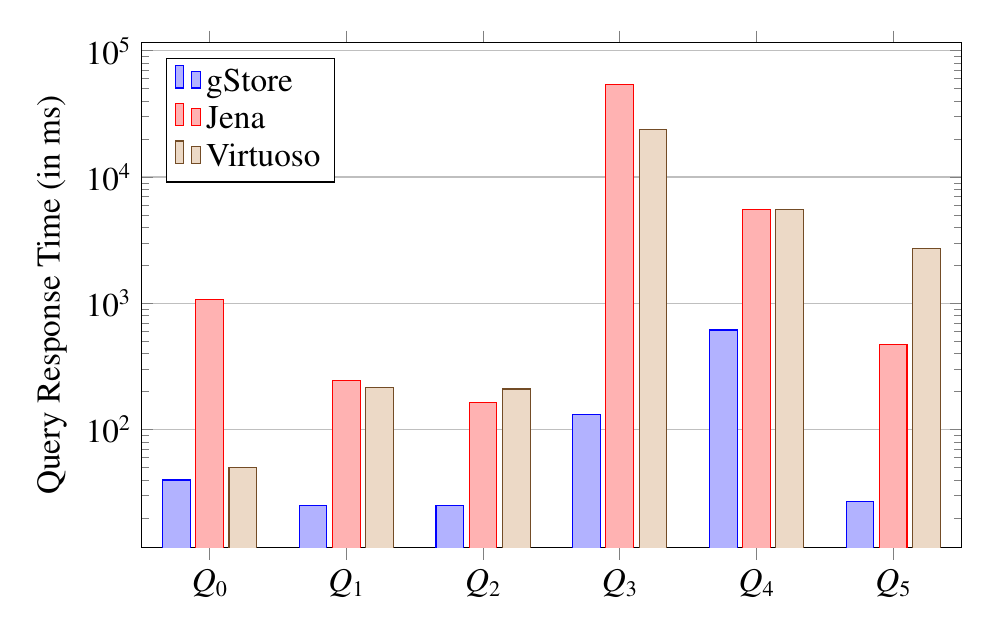
\begin{tikzpicture}[font=\large]
 		 \begin{semilogyaxis}[
 		   %width = 30cm,
 		   %height = 15cm,
 		   %ymax = 100000,
               width = 12cm,
               height = 8cm,
    			ybar,
    			%ymin = 1,
    			%ymax = 5000000000,
%    ytick = {1,10,100,1000,10000,100000,1000000,10000000},
   			ymajorgrids = true,
   			ylabel = {Query Response Time (in ms)},
                %xlabel = {Queries},
    			symbolic x coords = {$Q_0$,$Q_1$,$Q_2$,$Q_3$,$Q_4$,$Q_5$},
    			  %bar width=5pt,
    			  %enlarge x limits=0.02,
    			scaled y ticks = true,
			legend pos= north west,
 legend cell align=left
   		]
   \addplot coordinates {($Q_0$, 40) ($Q_1$, 25) ($Q_2$, 25) ($Q_3$, 131) ($Q_4$, 616) ($Q_5$, 27)};

   \addplot coordinates {($Q_0$, 1070) ($Q_1$, 245) ($Q_2$, 164) ($Q_3$, 53887) ($Q_4$, 5577) ($Q_5$, 469)};
   
   \addplot coordinates {($Q_0$, 50) ($Q_1$, 217) ($Q_2$, 210) ($Q_3$, 23797) ($Q_4$, 5536) ($Q_5$, 2736)};
		
   		 \legend{gStore,Jena, Virtuoso}
  		\end{semilogyaxis}
\end{tikzpicture}

		}
		\label{fig:dbpedia170MPerformance}%
	}
	\\
	\subfigure[dbpedia1B]{%
		\resizebox{\columnwidth}{!}{
				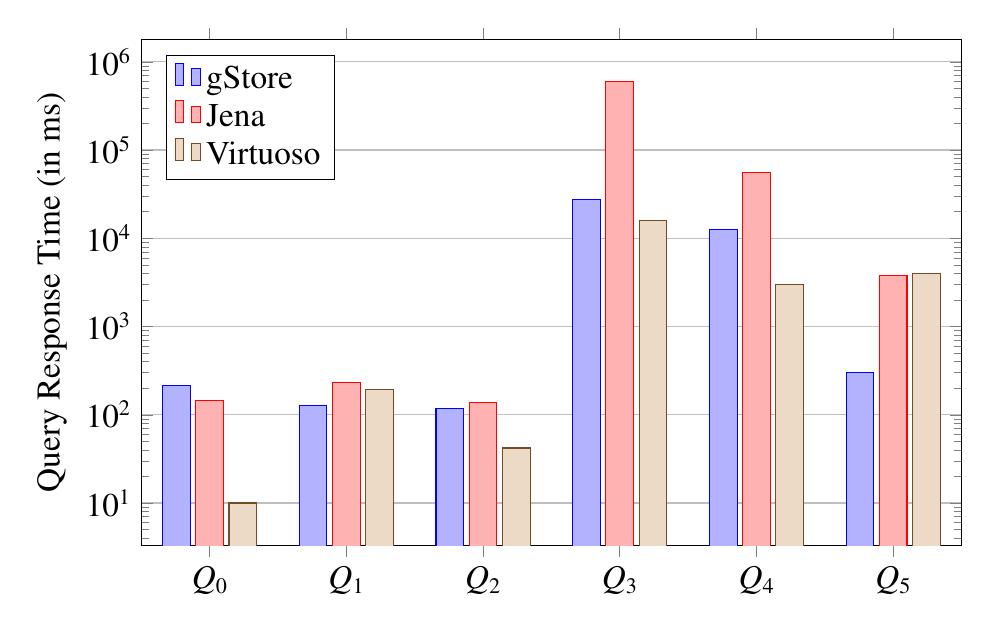
\begin{tikzpicture}[font=\large]
 		 \begin{semilogyaxis}[
 		   %width = 30cm,
 		   %height = 15cm,
 		   %ymax = 100000,
               width = 12cm,
               height = 8cm,
    			ybar,
    			%ymin = 1,
    			%ymax = 5000000000,
%    ytick = {1,10,100,1000,10000,100000,1000000,10000000},
   			ymajorgrids = true,
   			ylabel = {Query Response Time (in ms)},
                %xlabel = {Queries},
    			symbolic x coords = {$Q_0$,$Q_1$,$Q_2$,$Q_3$,$Q_4$,$Q_5$},
    			  %bar width=5pt,
    			  %enlarge x limits=0.02,
    			scaled y ticks = true,
			legend pos= north west,
 legend cell align=left
   		]
   \addplot coordinates {($Q_0$, 214) ($Q_1$, 128) ($Q_2$, 117) ($Q_3$, 27790) ($Q_4$, 12523) ($Q_5$, 302)};

   \addplot coordinates {($Q_0$, 146) ($Q_1$, 232) ($Q_2$, 137) ($Q_3$, 592110) ($Q_4$, 55723) ($Q_5$, 3803)};
   
   \addplot coordinates {($Q_0$, 10) ($Q_1$, 194) ($Q_2$, 42) ($Q_3$, 15752) ($Q_4$, 2990) ($Q_5$, 4004)};
		
   		 \legend{gStore,Jena, Virtuoso}
  		\end{semilogyaxis}
\end{tikzpicture}

		}
		\label{fig:dbpedia1BPerformance}%
	}%
	\caption{Query Performance over dbpedia170M and dbpedia1B}%
	\label{fig:dbpediaPerformance}
\end{figure}

\begin{figure}[t]%
	\subfigure[bsbm10M]{%
		\resizebox{\columnwidth}{!}{
				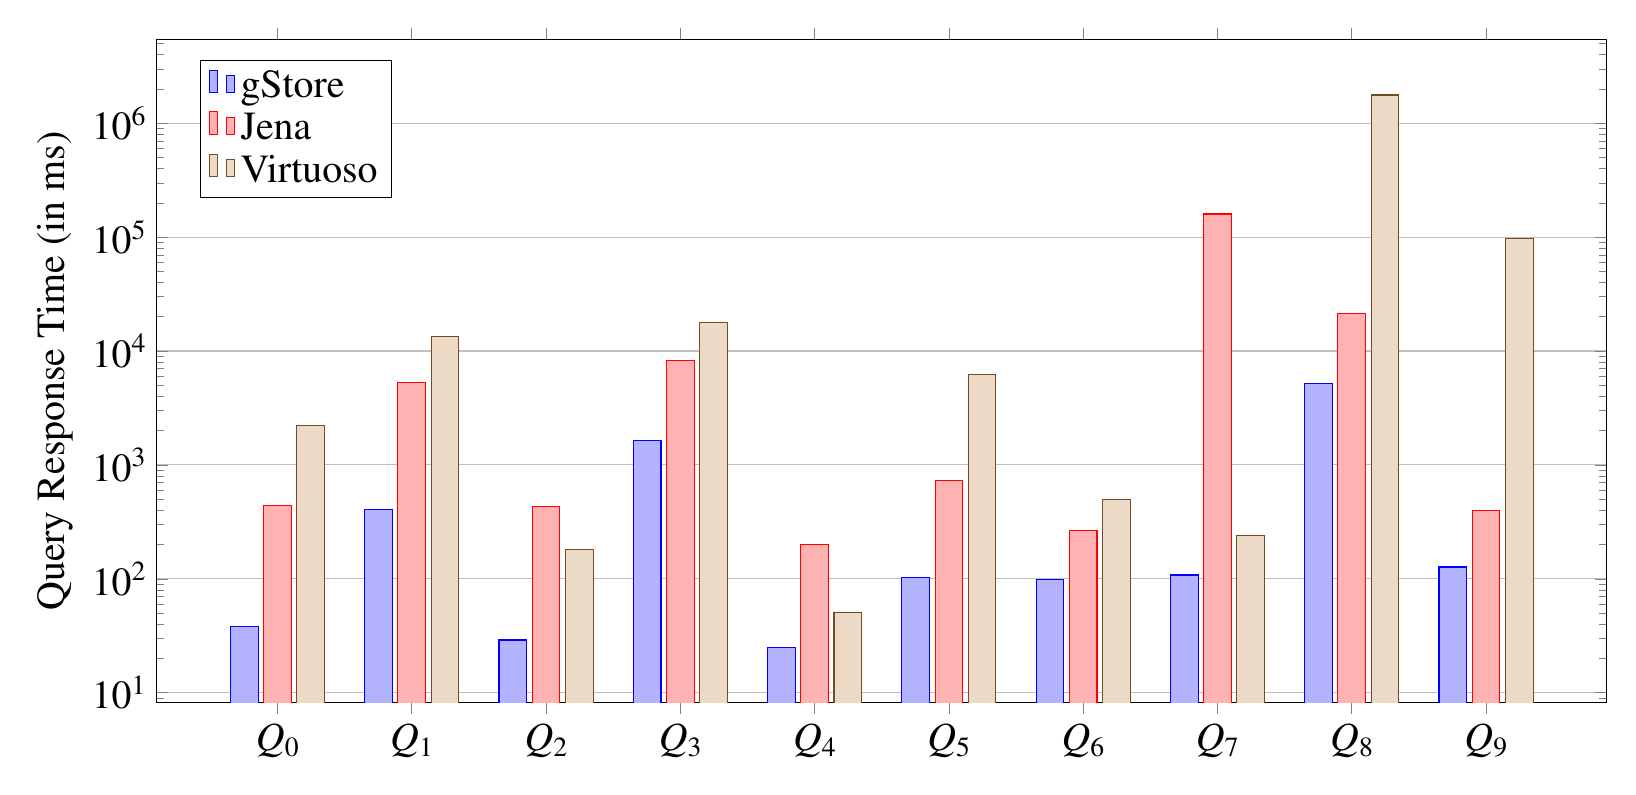
\begin{tikzpicture}[font=\Large]
 		 \begin{semilogyaxis}[
               width = 20cm,
               height = 10cm,
               %ymax = 100000,
    			ybar,
   			ymajorgrids = true,
   			ylabel = {Query Response Time (in ms)},
                %xlabel = {Queries},
    			symbolic x coords = {$Q_{0}$, $Q_{1}$,$Q_{2}$,$Q_{3}$,$Q_{4}$,$Q_{5}$,$Q_{6}$,$Q_{7}$,$Q_{8}$,$Q_{9}$},
    %bar width=5pt,
             %enlarge x limits=0.02,
    			scaled y ticks = true,
			legend pos= north west,
 legend cell align=left
   		]
   \addplot coordinates {($Q_{0}$, 38) ($Q_{1}$, 404) ($Q_{2}$, 29) ($Q_{3}$, 1635) ($Q_{4}$, 25) ($Q_{5}$, 103) ($Q_{6}$, 99) ($Q_{7}$, 108) ($Q_{8}$, 5148) ($Q_{9}$, 127)};


\addplot coordinates {($Q_{0}$, 441) ($Q_{1}$, 5333) ($Q_{2}$, 428) ($Q_{3}$, 8331) ($Q_{4}$, 200) ($Q_{5}$, 727) ($Q_{6}$, 267) ($Q_{7}$, 159700) ($Q_{8}$, 21462) ($Q_{9}$, 401)};
		
\addplot coordinates {($Q_{0}$, 2222) ($Q_{1}$, 13505) ($Q_{2}$, 180) ($Q_{3}$, 17779) ($Q_{4}$, 51) ($Q_{5}$, 6236) ($Q_{6}$, 500) ($Q_{7}$, 242) ($Q_{8}$, 1771450) ($Q_{9}$, 96463)};
		
%result num: 
%69724 3304145 0 3204145 0 65419 2011 45 12765738 520
		
   		 \legend{gStore,Jena, Virtuoso}
  		\end{semilogyaxis}
\end{tikzpicture}

		}
		\label{fig:bsbm10MPerformance}%
	}
	\\
	\subfigure[bsbm100M]{%
		\resizebox{\columnwidth}{!}{
				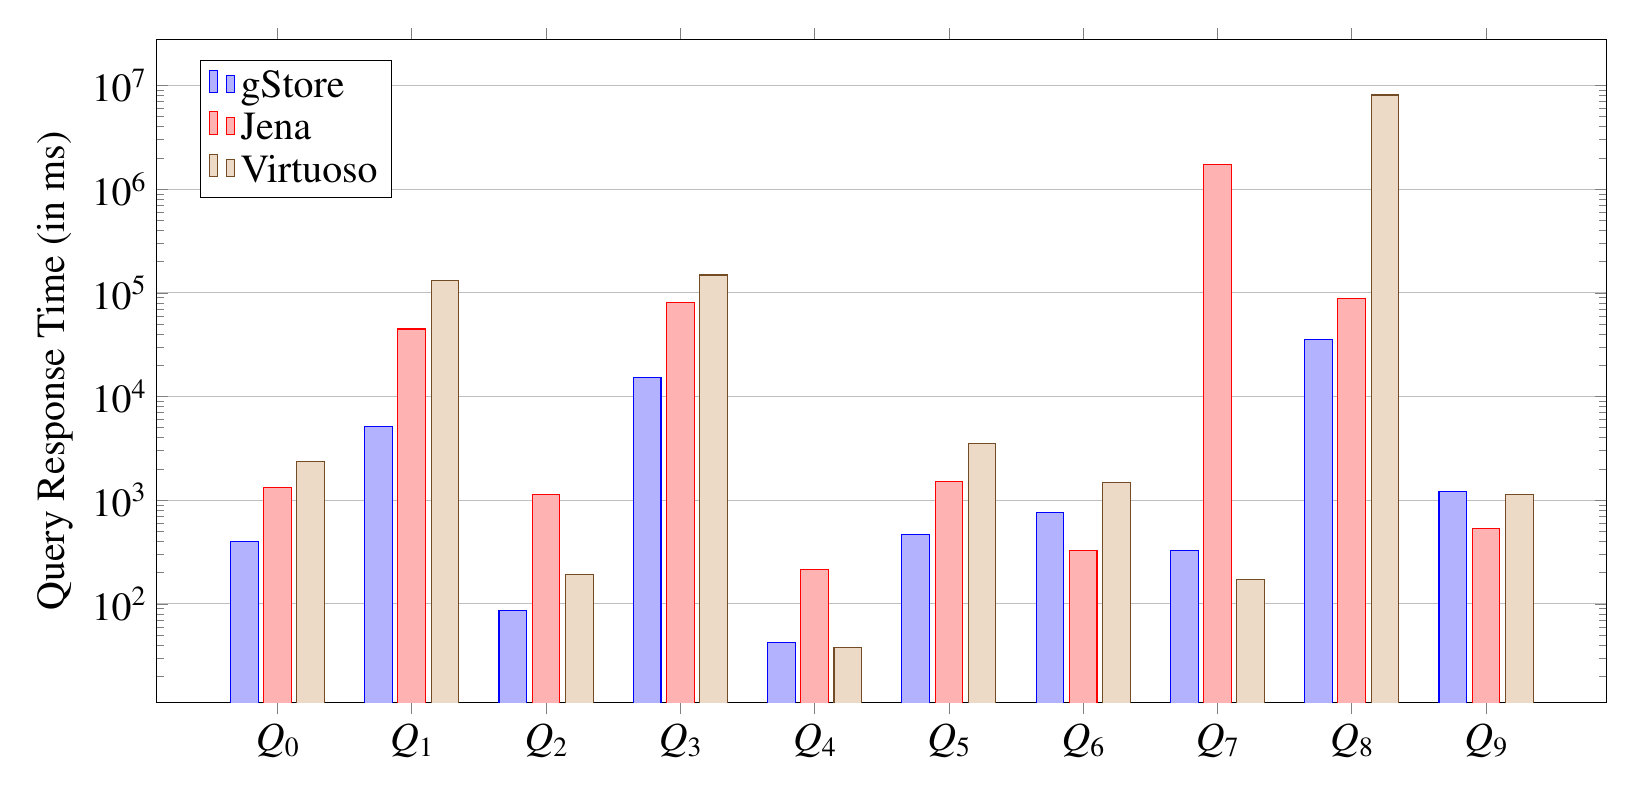
\begin{tikzpicture}[font=\Large]
 		 \begin{semilogyaxis}[
               width = 20cm,
               height = 10cm,
               %ymax = 100000,
    			ybar,
   			ymajorgrids = true,
   			ylabel = {Query Response Time (in ms)},
                %xlabel = {Queries},
    			symbolic x coords = {$Q_{0}$, $Q_{1}$,$Q_{2}$,$Q_{3}$,$Q_{4}$,$Q_{5}$,$Q_{6}$,$Q_{7}$,$Q_{8}$,$Q_{9}$},
    %bar width=5pt,
             %enlarge x limits=0.02,
    			scaled y ticks = true,
			legend pos= north west,
 legend cell align=left
   		]
   \addplot coordinates {($Q_{0}$, 403) ($Q_{1}$, 5153) ($Q_{2}$, 86) ($Q_{3}$, 15358) ($Q_{4}$, 42) ($Q_{5}$, 467) ($Q_{6}$, 754) ($Q_{7}$, 329) ($Q_{8}$, 35169) ($Q_{9}$, 1216)};


\addplot coordinates {($Q_{0}$, 1329) ($Q_{1}$, 44767) ($Q_{2}$, 1124) ($Q_{3}$, 80432) ($Q_{4}$, 213) ($Q_{5}$, 1513) ($Q_{6}$, 327) ($Q_{7}$, 1744878) ($Q_{8}$, 88664) ($Q_{9}$, 538)};
		
\addplot coordinates {($Q_{0}$, 2353) ($Q_{1}$, 130748) ($Q_{2}$, 190) ($Q_{3}$, 148439) ($Q_{4}$, 38) ($Q_{5}$, 3504) ($Q_{6}$, 1494) ($Q_{7}$, 173) ($Q_{8}$, 8102026) ($Q_{9}$, 1139)};
		
%result num: 
%69724 3304145 0 3204145 0 65419 2011 45 12765738 520
		
   		 \legend{gStore,Jena, Virtuoso}
  		\end{semilogyaxis}
\end{tikzpicture}

		}
		\label{fig:bsbm100MPerformance}%
	}%
	\caption{Query Performance over BSBM 10M and 100M}%
	\label{fig:bsbmPerformance1}
\end{figure}

\begin{figure}[t]%
	\subfigure[bsbm200M]{%
		\resizebox{\columnwidth}{!}{
				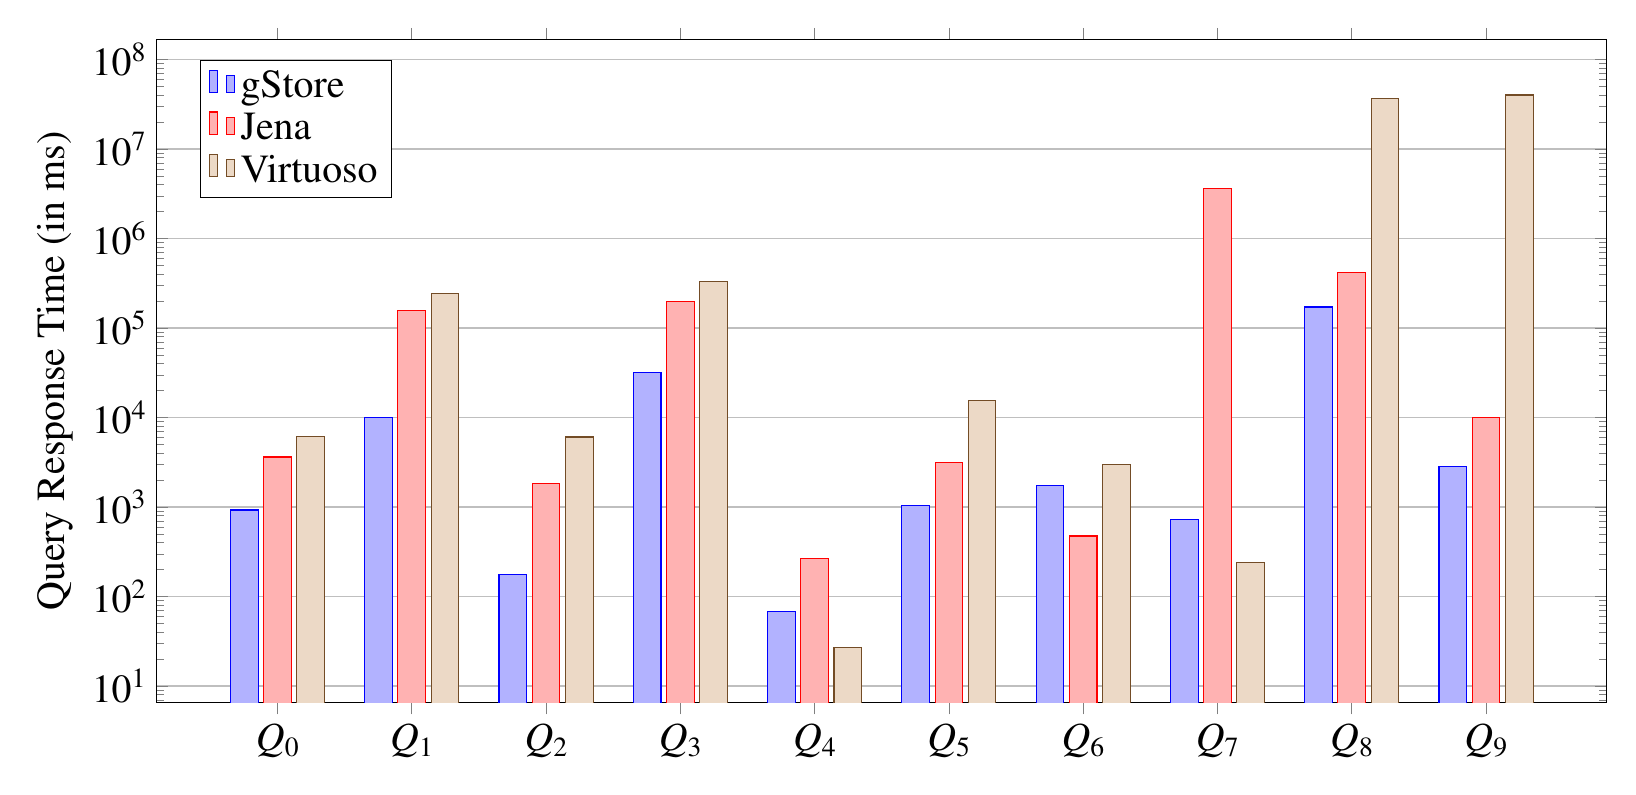
\begin{tikzpicture}[font=\Large]
 		 \begin{semilogyaxis}[
               width = 20cm,
               height = 10cm,
               %ymax = 100000,
    			ybar,
   			ymajorgrids = true,
   			ylabel = {Query Response Time (in ms)},
                %xlabel = {Queries},
    			symbolic x coords = {$Q_{0}$, $Q_{1}$,$Q_{2}$,$Q_{3}$,$Q_{4}$,$Q_{5}$,$Q_{6}$,$Q_{7}$,$Q_{8}$,$Q_{9}$},
    %bar width=5pt,
             %enlarge x limits=0.02,
    			scaled y ticks = true,
			legend pos= north west,
 legend cell align=left
   		]
   \addplot coordinates {($Q_{0}$, 927) ($Q_{1}$, 9974) ($Q_{2}$, 177) ($Q_{3}$, 31672) ($Q_{4}$, 68) ($Q_{5}$, 1037) ($Q_{6}$, 1756) ($Q_{7}$, 725) ($Q_{8}$, 171876) ($Q_{9}$, 2850)};


\addplot coordinates {($Q_{0}$, 3623) ($Q_{1}$, 157846) ($Q_{2}$, 1841) ($Q_{3}$, 199087) ($Q_{4}$, 266) ($Q_{5}$, 3176) ($Q_{6}$, 474) ($Q_{7}$, 3635906) ($Q_{8}$, 415252) ($Q_{9}$, 9893)};
		
\addplot coordinates {($Q_{0}$, 6121) ($Q_{1}$, 241390) ($Q_{2}$, 6053) ($Q_{3}$, 329311) ($Q_{4}$, 27) ($Q_{5}$, 15532) ($Q_{6}$, 3007) ($Q_{7}$, 242) ($Q_{8}$, 36615810) ($Q_{9}$, 40180121)};
		
%result num: 
%69724 3304145 0 3204145 0 65419 2011 45 12765738 520
		
   		 \legend{gStore,Jena, Virtuoso}
  		\end{semilogyaxis}
\end{tikzpicture}

		}
		\label{fig:bsbm200MPerformance}%
	}%
	\\
	\subfigure[bsbm300M]{%
		\resizebox{\columnwidth}{!}{
				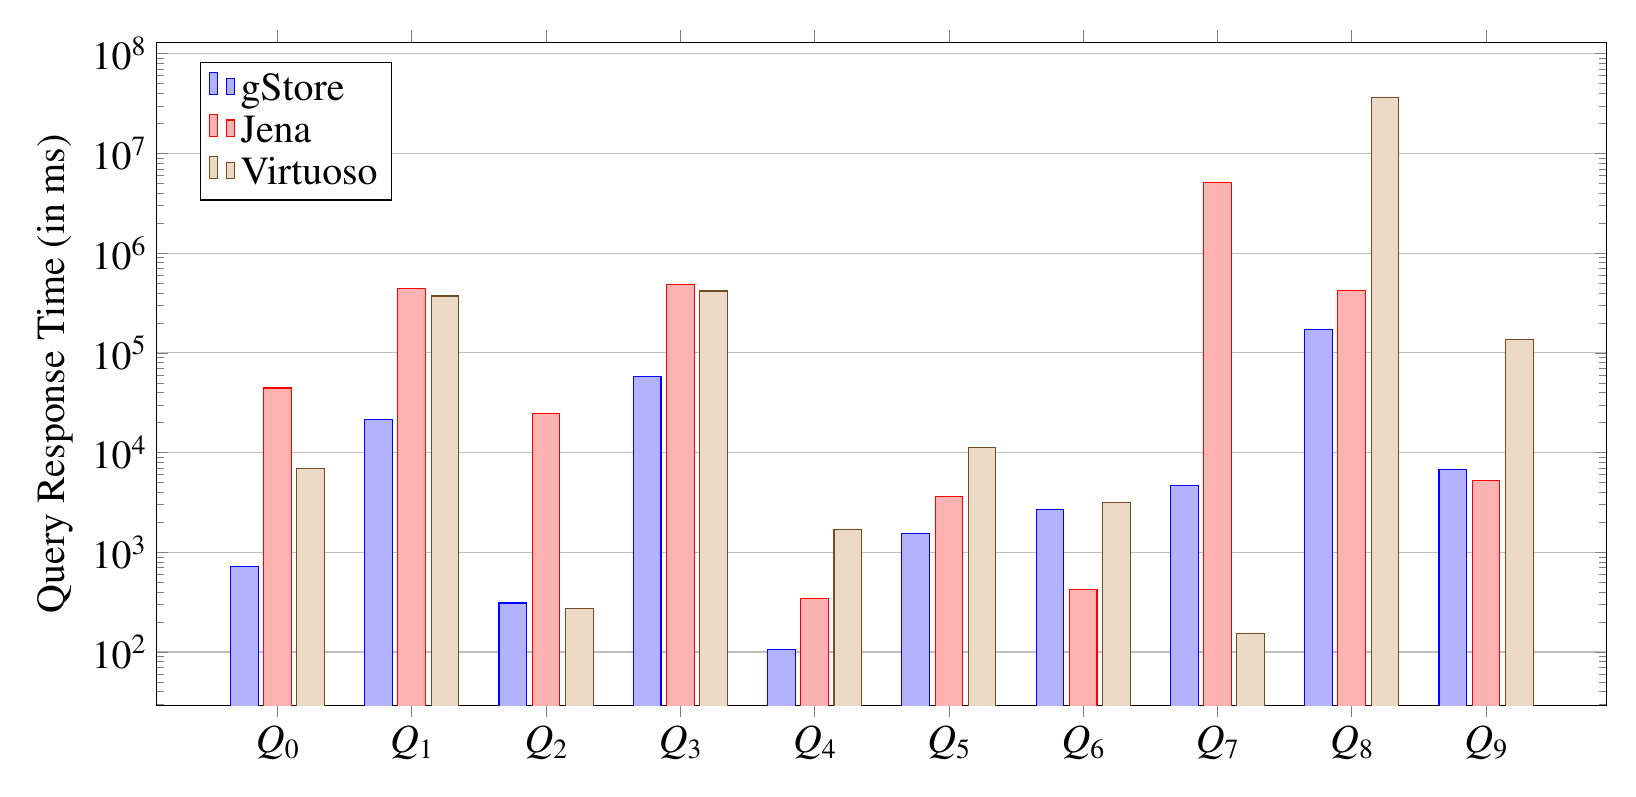
\begin{tikzpicture}[font=\Large]
 		 \begin{semilogyaxis}[
               width = 20cm,
               height = 10cm,
               %ymax = 100000,
    			ybar,
   			ymajorgrids = true,
   			ylabel = {Query Response Time (in ms)},
                %xlabel = {Queries},
    			symbolic x coords = {$Q_{0}$, $Q_{1}$,$Q_{2}$,$Q_{3}$,$Q_{4}$,$Q_{5}$,$Q_{6}$,$Q_{7}$,$Q_{8}$,$Q_{9}$},
    %bar width=5pt,
             %enlarge x limits=0.02,
    			scaled y ticks = true,
			legend pos= north west,
 legend cell align=left
   		]
   \addplot coordinates {($Q_{0}$, 724) ($Q_{1}$, 21516) ($Q_{2}$, 310) ($Q_{3}$, 57998) ($Q_{4}$, 105) ($Q_{5}$, 1558) ($Q_{6}$, 2659) ($Q_{7}$, 4633) ($Q_{8}$, 171335) ($Q_{9}$, 6697)};


\addplot coordinates {($Q_{0}$, 44359) ($Q_{1}$, 441665) ($Q_{2}$, 24686) ($Q_{3}$, 486898) ($Q_{4}$, 343) ($Q_{5}$, 3638) ($Q_{6}$, 426) ($Q_{7}$, 5151957) ($Q_{8}$, 417837) ($Q_{9}$, 5252)};

\addplot coordinates {($Q_{0}$, 6981) ($Q_{1}$, 371534) ($Q_{2}$, 273) ($Q_{3}$, 416788) ($Q_{4}$, 1679) ($Q_{5}$, 11308) ($Q_{6}$, 3151) ($Q_{7}$, 153) ($Q_{8}$, 36322654) ($Q_{9}$, 137430)};
		
%result num: 
%69724 3304145 0 3204145 0 65419 2011 45 12765738 520
		
   		 \legend{gStore,Jena, Virtuoso}
  		\end{semilogyaxis}
\end{tikzpicture}

		}
		\label{fig:bsbm300MPerformance}%
	}%
	\caption{Query Performance over BSBM 200M and 300M}%
	\label{fig:bsbmPerformance2}
\end{figure}

\begin{figure}[t]%
	\subfigure[bsbm500M]{%
		\resizebox{\columnwidth}{!}{
				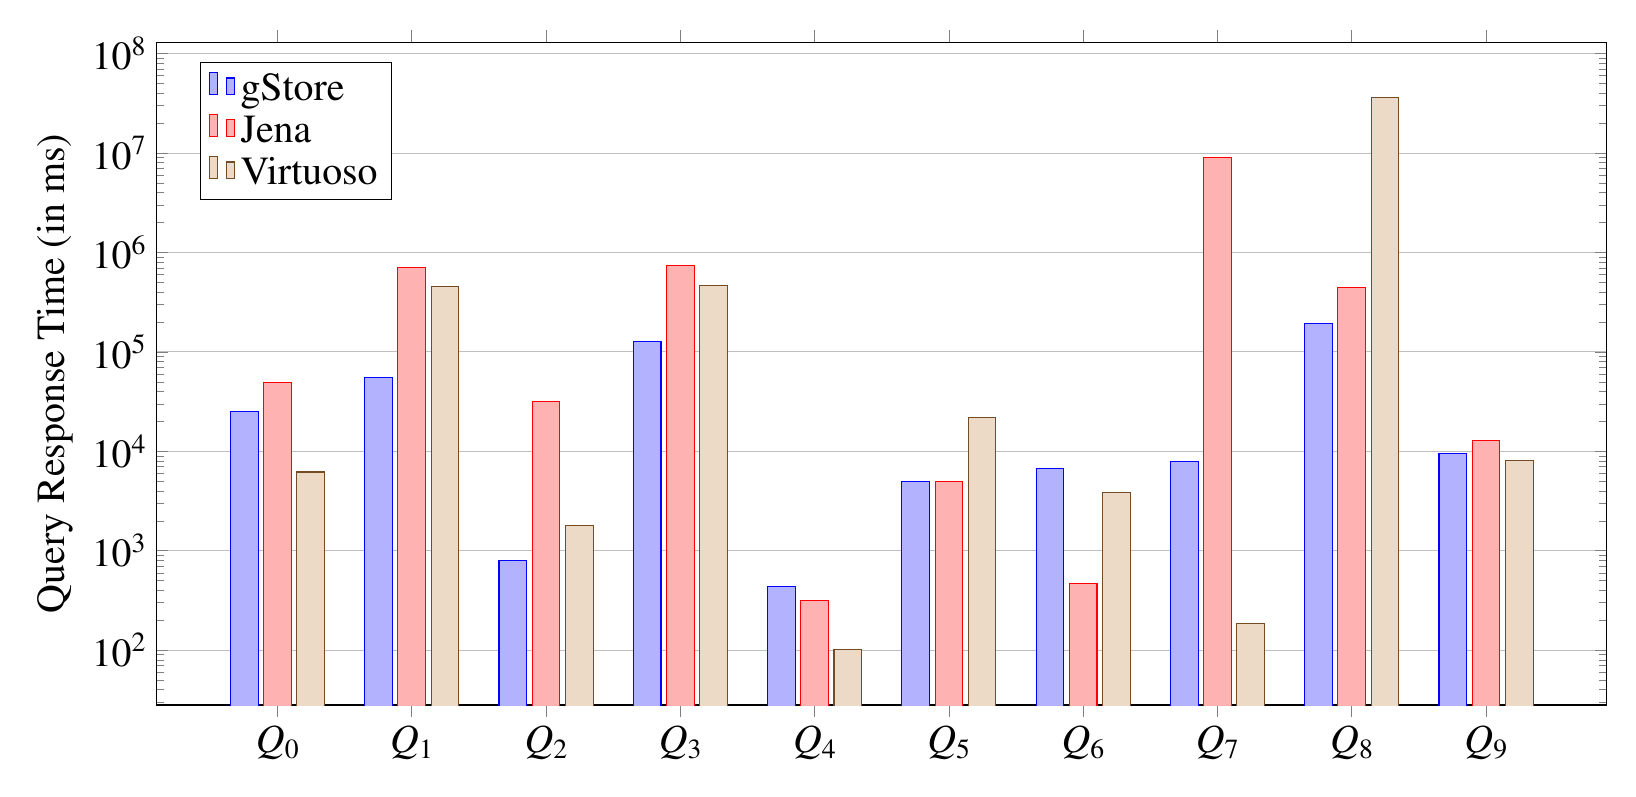
\begin{tikzpicture}[font=\Large]
 		 \begin{semilogyaxis}[
               width = 20cm,
               height = 10cm,
               %ymax = 100000,
    			ybar,
   			ymajorgrids = true,
   			ylabel = {Query Response Time (in ms)},
                %xlabel = {Queries},
    			symbolic x coords = {$Q_{0}$, $Q_{1}$,$Q_{2}$,$Q_{3}$,$Q_{4}$,$Q_{5}$,$Q_{6}$,$Q_{7}$,$Q_{8}$,$Q_{9}$},
    %bar width=5pt,
             %enlarge x limits=0.02,
    			scaled y ticks = true,
			legend pos= north west,
 legend cell align=left
   		]
   \addplot coordinates {($Q_{0}$, 24980) ($Q_{1}$, 54830) ($Q_{2}$, 797) ($Q_{3}$, 126361) ($Q_{4}$, 439) ($Q_{5}$, 4961) ($Q_{6}$, 6703) ($Q_{7}$, 7863) ($Q_{8}$, 195127) ($Q_{9}$, 9428)};


\addplot coordinates {($Q_{0}$, 48923) ($Q_{1}$, 706555) ($Q_{2}$, 31953) ($Q_{3}$, 735042) ($Q_{4}$, 315) ($Q_{5}$, 5013) ($Q_{6}$, 471) ($Q_{7}$, 8937023) ($Q_{8}$, 445969) ($Q_{9}$, 12882)};

\addplot coordinates {($Q_{0}$, 6204) ($Q_{1}$, 450346) ($Q_{2}$, 1805) ($Q_{3}$, 462376) ($Q_{4}$, 101) ($Q_{5}$, 21968) ($Q_{6}$, 3892) ($Q_{7}$, 184) ($Q_{8}$, 36326080) ($Q_{9}$, 8162)};

		
%result num: 
%69724 3304145 0 3204145 0 65419 2011 45 12765738 520
		
   		 \legend{gStore,Jena, Virtuoso}
  		\end{semilogyaxis}
\end{tikzpicture}

		}
		\label{fig:bsbm500MPerformance}%
	}%
	\caption{Query Performance over BSBM 500M}%
	\label{fig:bsbmPerformance3}
\end{figure}

%\clearpage

\begin{figure}[t]%
	\subfigure[lubm10M]{%
		\resizebox{\columnwidth}{!}{
				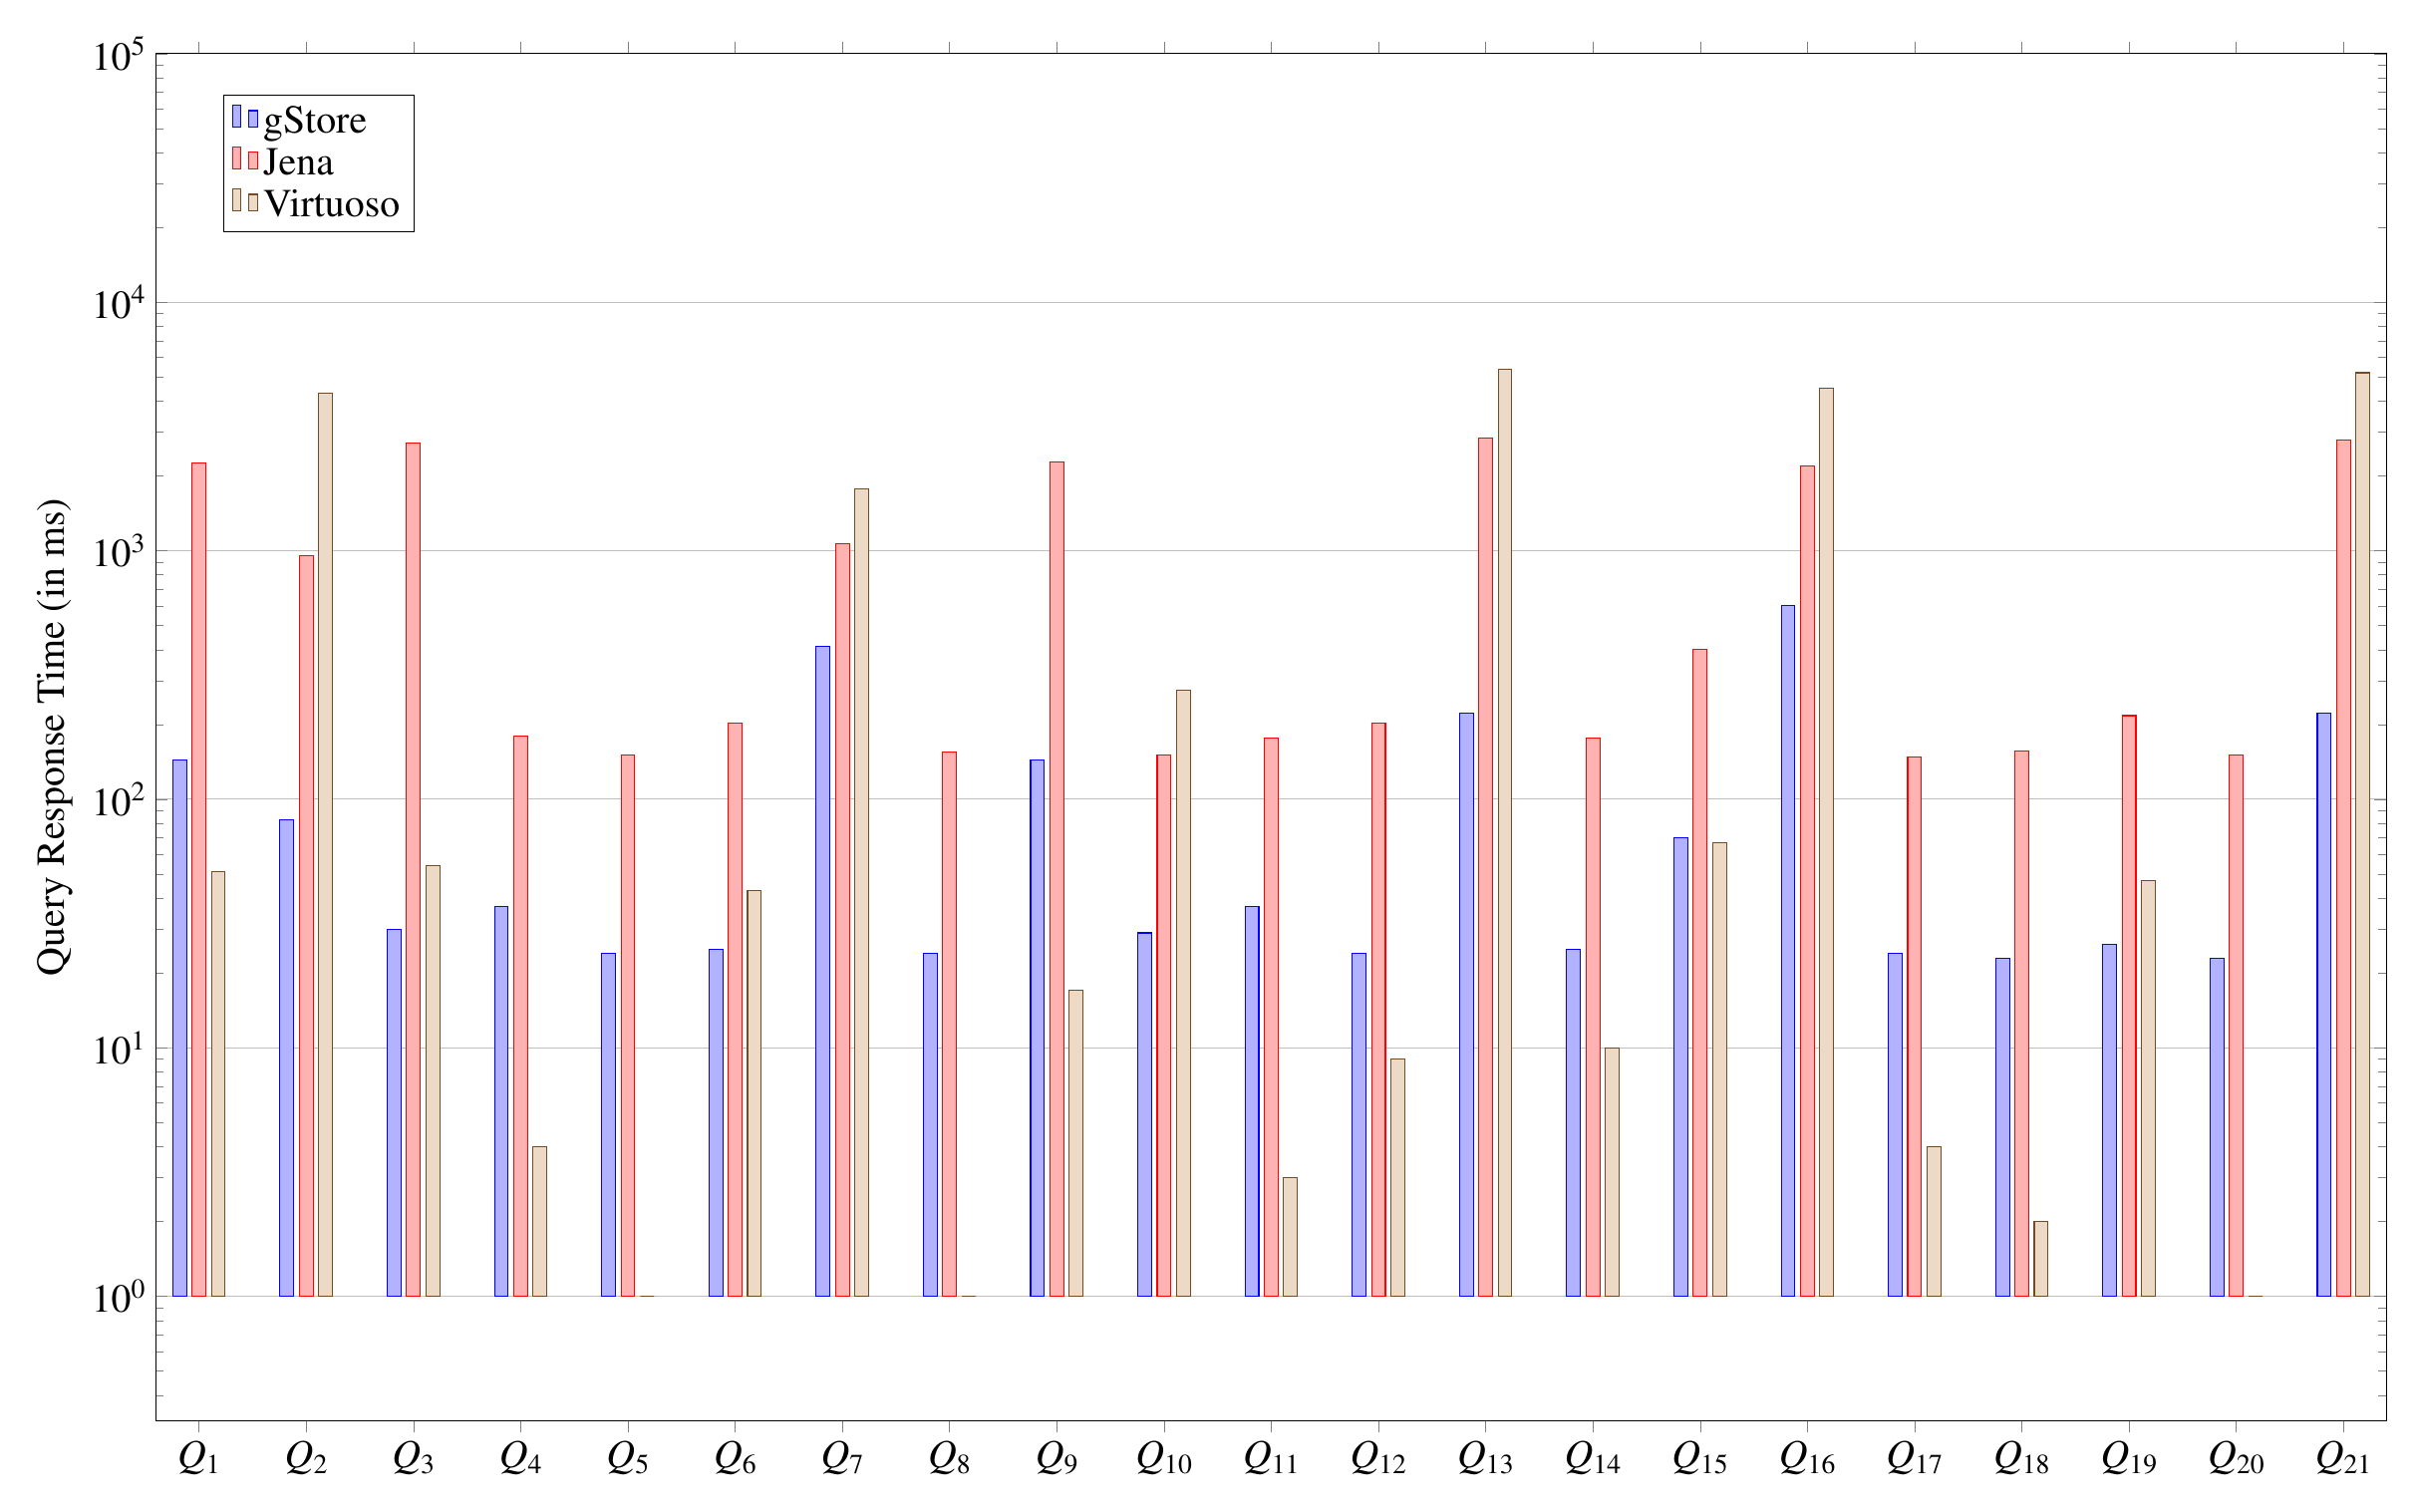
\begin{tikzpicture}[font=\Large]
 		 \begin{semilogyaxis}[
               width = 30cm,
               height = 19cm,
               ymax = 100000,
    			ybar,
   			ymajorgrids = true,
   			ylabel = {Query Response Time (in ms)},
                %xlabel = {Queries},
    			symbolic x coords = {$Q_{1}$,$Q_{2}$,$Q_{3}$,$Q_{4}$,$Q_{5}$,$Q_{6}$,$Q_{7}$,$Q_{8}$,$Q_{9}$,$Q_{10}$,$Q_{11}$,$Q_{12}$,$Q_{13}$,$Q_{14}$,$Q_{15}$,$Q_{16}$,$Q_{17}$,$Q_{18}$,$Q_{19}$,$Q_{20}$,$Q_{21}$},
    bar width=5pt,
             enlarge x limits=0.02,
    			scaled y ticks = true,
			legend pos= north west,
 legend cell align=left
   		]
   \addplot coordinates {($Q_{1}$, 144) ($Q_{2}$, 83) ($Q_{3}$, 30) ($Q_{4}$, 37) ($Q_{5}$, 24) ($Q_{6}$, 25) ($Q_{7}$, 413) ($Q_{8}$, 24) ($Q_{9}$, 144) ($Q_{10}$, 29) ($Q_{11}$, 37) ($Q_{12}$, 24) ($Q_{13}$, 223) ($Q_{14}$, 25) ($Q_{15}$, 70) ($Q_{16}$, 602) ($Q_{17}$, 24) ($Q_{18}$, 23) ($Q_{19}$, 26) ($Q_{20}$, 23) ($Q_{21}$, 223)};


\addplot coordinates {($Q_{1}$, 2258) ($Q_{2}$, 953) ($Q_{3}$, 2715) ($Q_{4}$, 179) ($Q_{5}$, 151) ($Q_{6}$, 202) ($Q_{7}$, 1065) ($Q_{8}$, 155) ($Q_{9}$, 2274) ($Q_{10}$, 151) ($Q_{11}$, 177) ($Q_{12}$, 203) ($Q_{13}$, 2833) ($Q_{14}$, 177) ($Q_{15}$, 400) ($Q_{16}$, 2194) ($Q_{17}$, 148) ($Q_{18}$, 157) ($Q_{19}$, 217) ($Q_{20}$, 151) ($Q_{21}$, 2790)};
		
\addplot coordinates {($Q_{1}$, 51) ($Q_{2}$, 4287) ($Q_{3}$, 54) ($Q_{4}$, 4) ($Q_{5}$, 1) ($Q_{6}$, 43) ($Q_{7}$, 1770) ($Q_{8}$, 1) ($Q_{9}$, 17) ($Q_{10}$, 275) ($Q_{11}$, 3) ($Q_{12}$, 9) ($Q_{13}$, 5377) ($Q_{14}$, 10) ($Q_{15}$, 67) ($Q_{16}$, 4504) ($Q_{17}$, 4) ($Q_{18}$, 2) ($Q_{19}$, 47) ($Q_{20}$, 1) ($Q_{21}$, 5199)};
		
   		 \legend{gStore,Jena, Virtuoso}
  		\end{semilogyaxis}
\end{tikzpicture}

		}
		\label{fig:lubm10MPerformance}%
	}
	\\
	\subfigure[lubm100M]{%
		\resizebox{\columnwidth}{!}{
				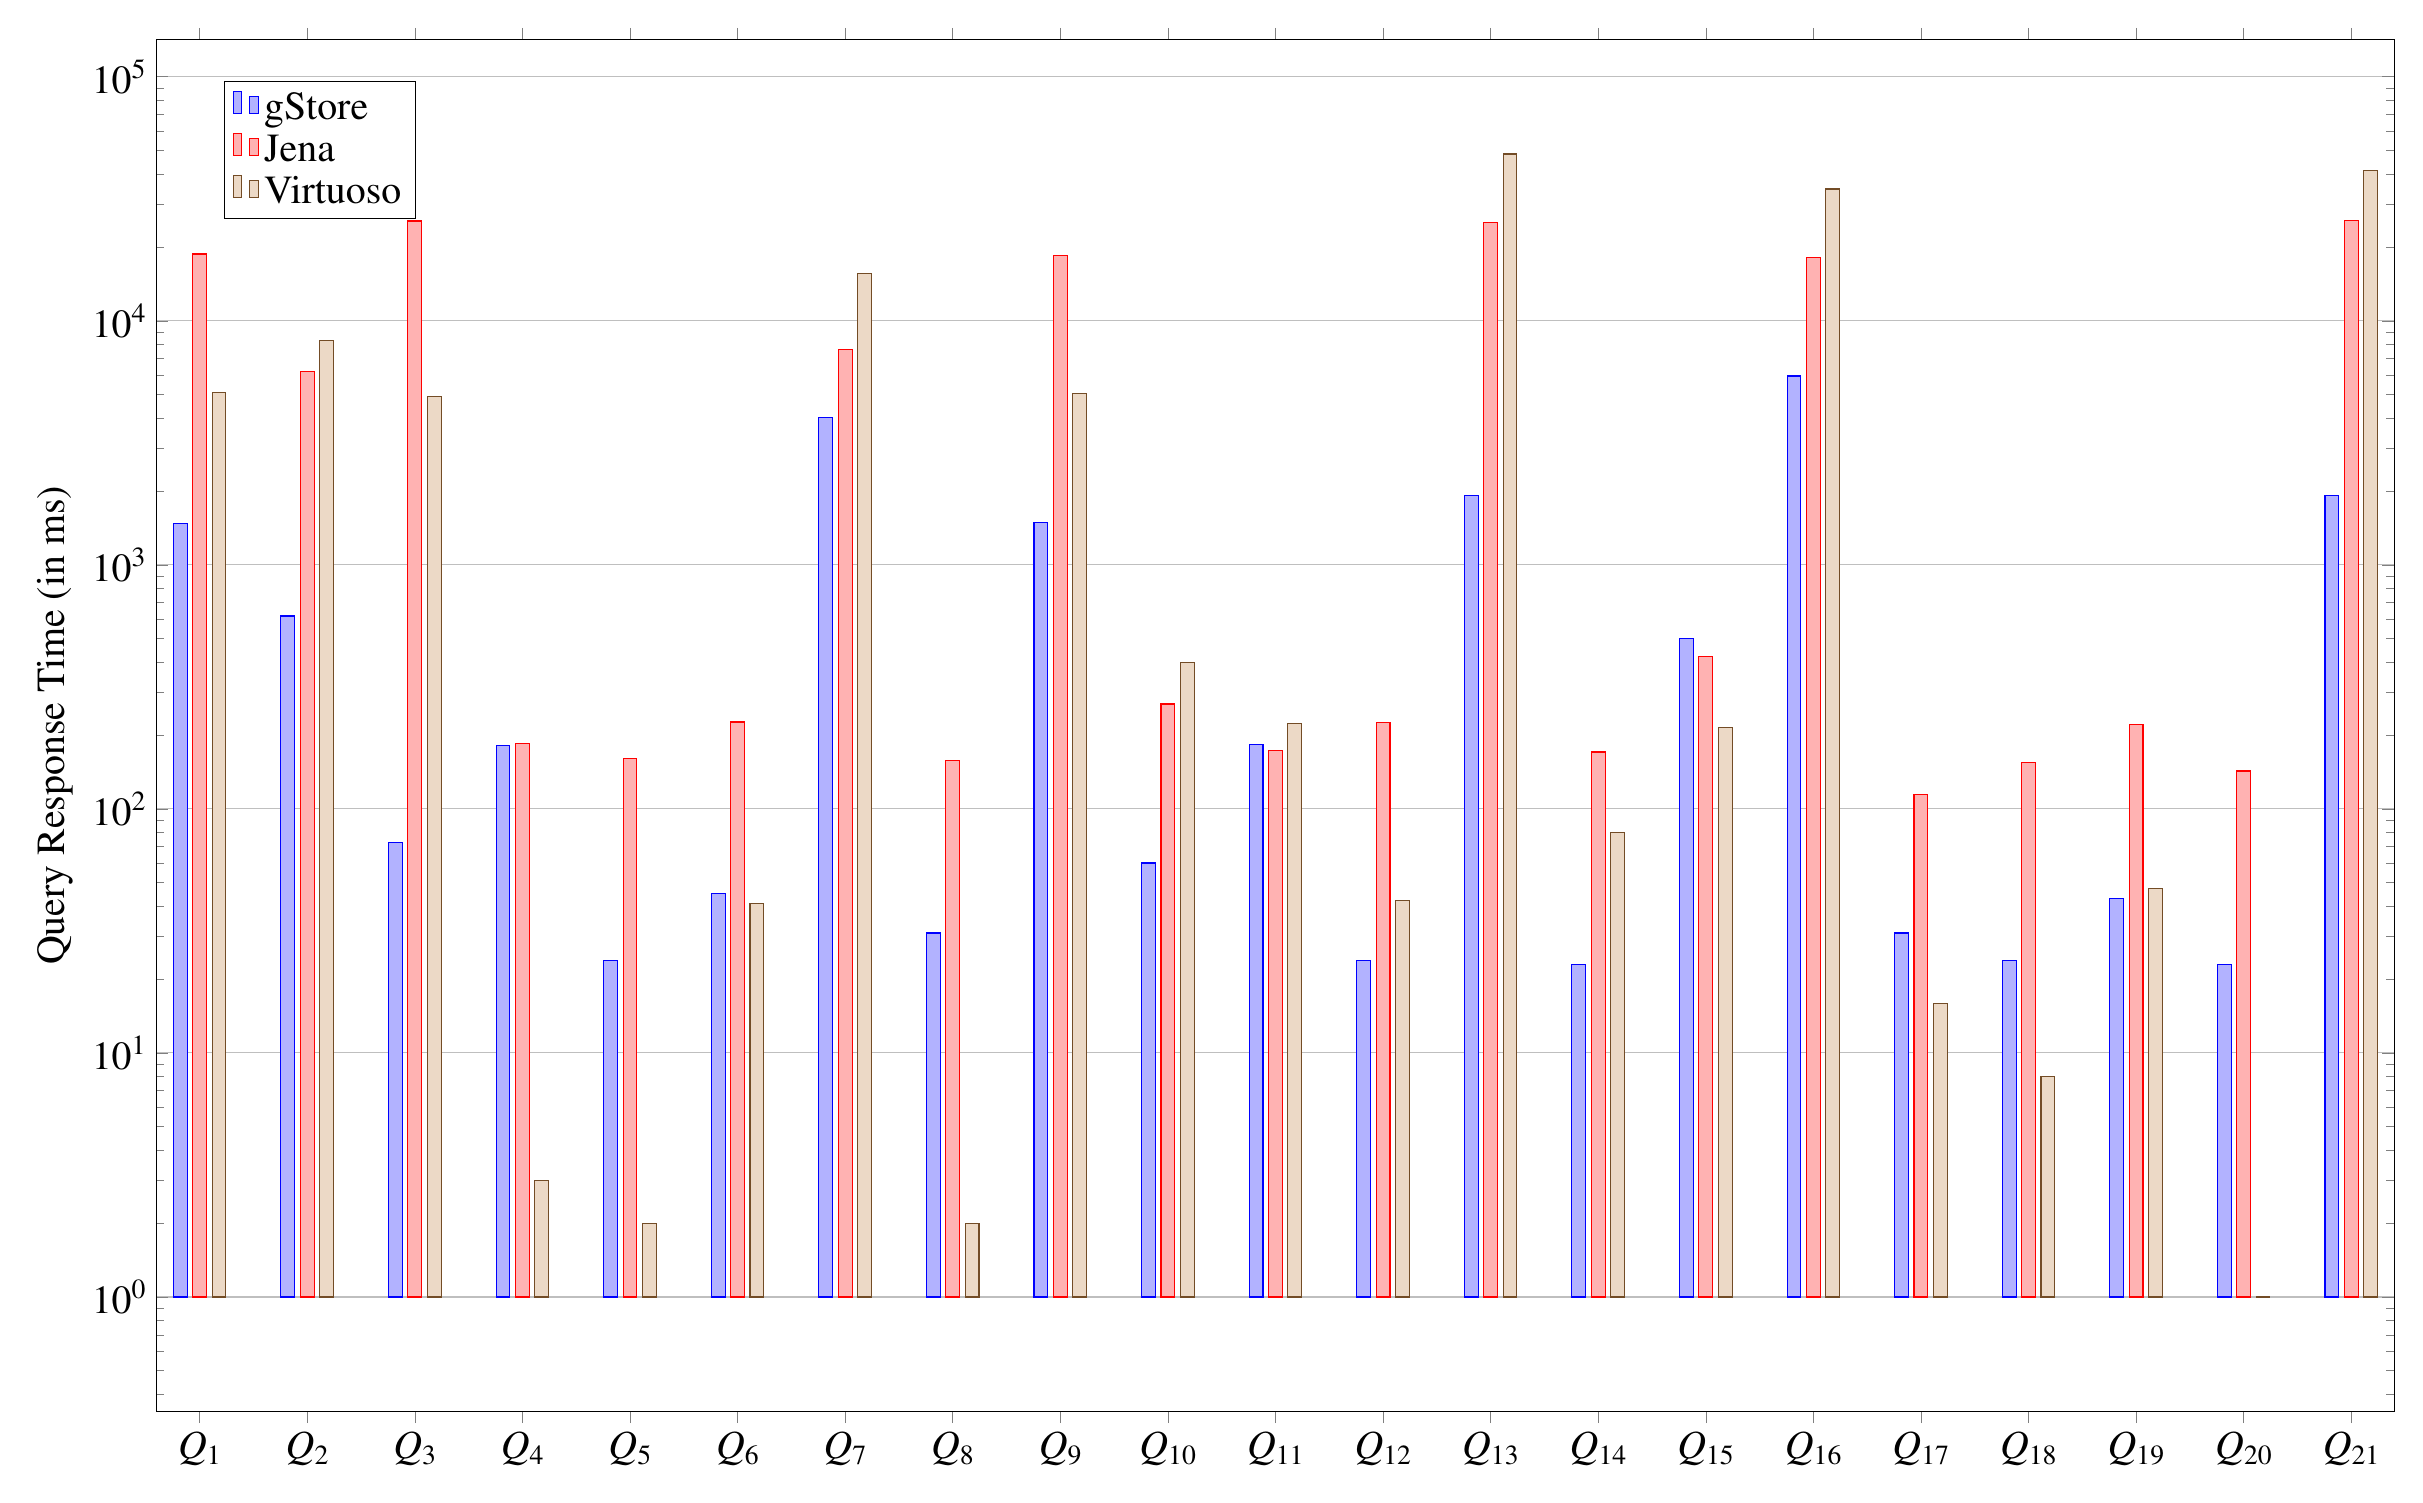
\begin{tikzpicture}[font=\Large]
 		 \begin{semilogyaxis}[
               width = 30cm,
               height = 19cm ,
    			ybar,
   			ymajorgrids = true,
   			ylabel = {Query Response Time (in ms)},
                %xlabel = {Queries},
    			symbolic x coords = 
    			{$Q_{1}$,$Q_{2}$,$Q_{3}$,$Q_{4}$,$Q_{5}$,$Q_{6}$,$Q_{7}$,$Q_{8}$,$Q_{9}$,$Q_{10}$,$Q_{11}$,$Q_{12}$,$Q_{13}$,$Q_{14}$,$Q_{15}$,$Q_{16}$,$Q_{17}$,$Q_{18}$,$Q_{19}$,$Q_{20}$,$Q_{21}$},
    bar width=5pt,
             enlarge x limits=0.02,
    			scaled y ticks = true,
			legend pos= north west,
 legend cell align=left
   		]
  \addplot coordinates {($Q_{1}$, 1478) ($Q_{2}$, 617) ($Q_{3}$, 73) ($Q_{4}$, 182) ($Q_{5}$, 24) ($Q_{6}$, 45) ($Q_{7}$, 4011) ($Q_{8}$, 31) ($Q_{9}$, 1495) ($Q_{10}$, 60) ($Q_{11}$, 183) ($Q_{12}$, 24) ($Q_{13}$, 1920) ($Q_{14}$, 23) ($Q_{15}$, 500) ($Q_{16}$, 5941) ($Q_{17}$, 31) ($Q_{18}$, 24) ($Q_{19}$, 43) ($Q_{20}$, 23) ($Q_{21}$, 1916)};
  
  
  \addplot coordinates {($Q_{1}$, 18776) ($Q_{2}$, 6219) ($Q_{3}$, 25643) ($Q_{4}$, 186) ($Q_{5}$, 161) ($Q_{6}$, 227) ($Q_{7}$, 7644) ($Q_{8}$, 158) ($Q_{9}$, 18533) ($Q_{10}$, 269) ($Q_{11}$, 173) ($Q_{12}$, 226) ($Q_{13}$, 25385) ($Q_{14}$, 171) ($Q_{15}$, 420) ($Q_{16}$, 18165) ($Q_{17}$, 115) ($Q_{18}$, 155) ($Q_{19}$, 221) ($Q_{20}$, 143) ($Q_{21}$, 25749)};
  
  \addplot coordinates {($Q_{1}$, 5100) ($Q_{2}$, 8292) ($Q_{3}$, 4909) ($Q_{4}$, 3) ($Q_{5}$, 2) ($Q_{6}$, 41) ($Q_{7}$, 15666) ($Q_{8}$, 2) ($Q_{9}$, 5048) ($Q_{10}$, 399) ($Q_{11}$, 224) ($Q_{12}$, 42) ($Q_{13}$, 48231) ($Q_{14}$, 80) ($Q_{15}$, 216) ($Q_{16}$, 34674) ($Q_{17}$, 16) ($Q_{18}$, 8) ($Q_{19}$, 47) ($Q_{20}$, 1) ($Q_{21}$, 41313)};
		
   		 \legend{gStore,Jena, Virtuoso}
  		\end{semilogyaxis}
\end{tikzpicture}

		}
		\label{fig:lubm100MPerformance}%
	}%
	\caption{Query Performance over LUBM 10M and 100M}%
	\label{fig:lubmPerformance1}
\end{figure}
	
\begin{figure}[t]%
		\subfigure[lubm200M]{%
			\resizebox{\columnwidth}{!}{
					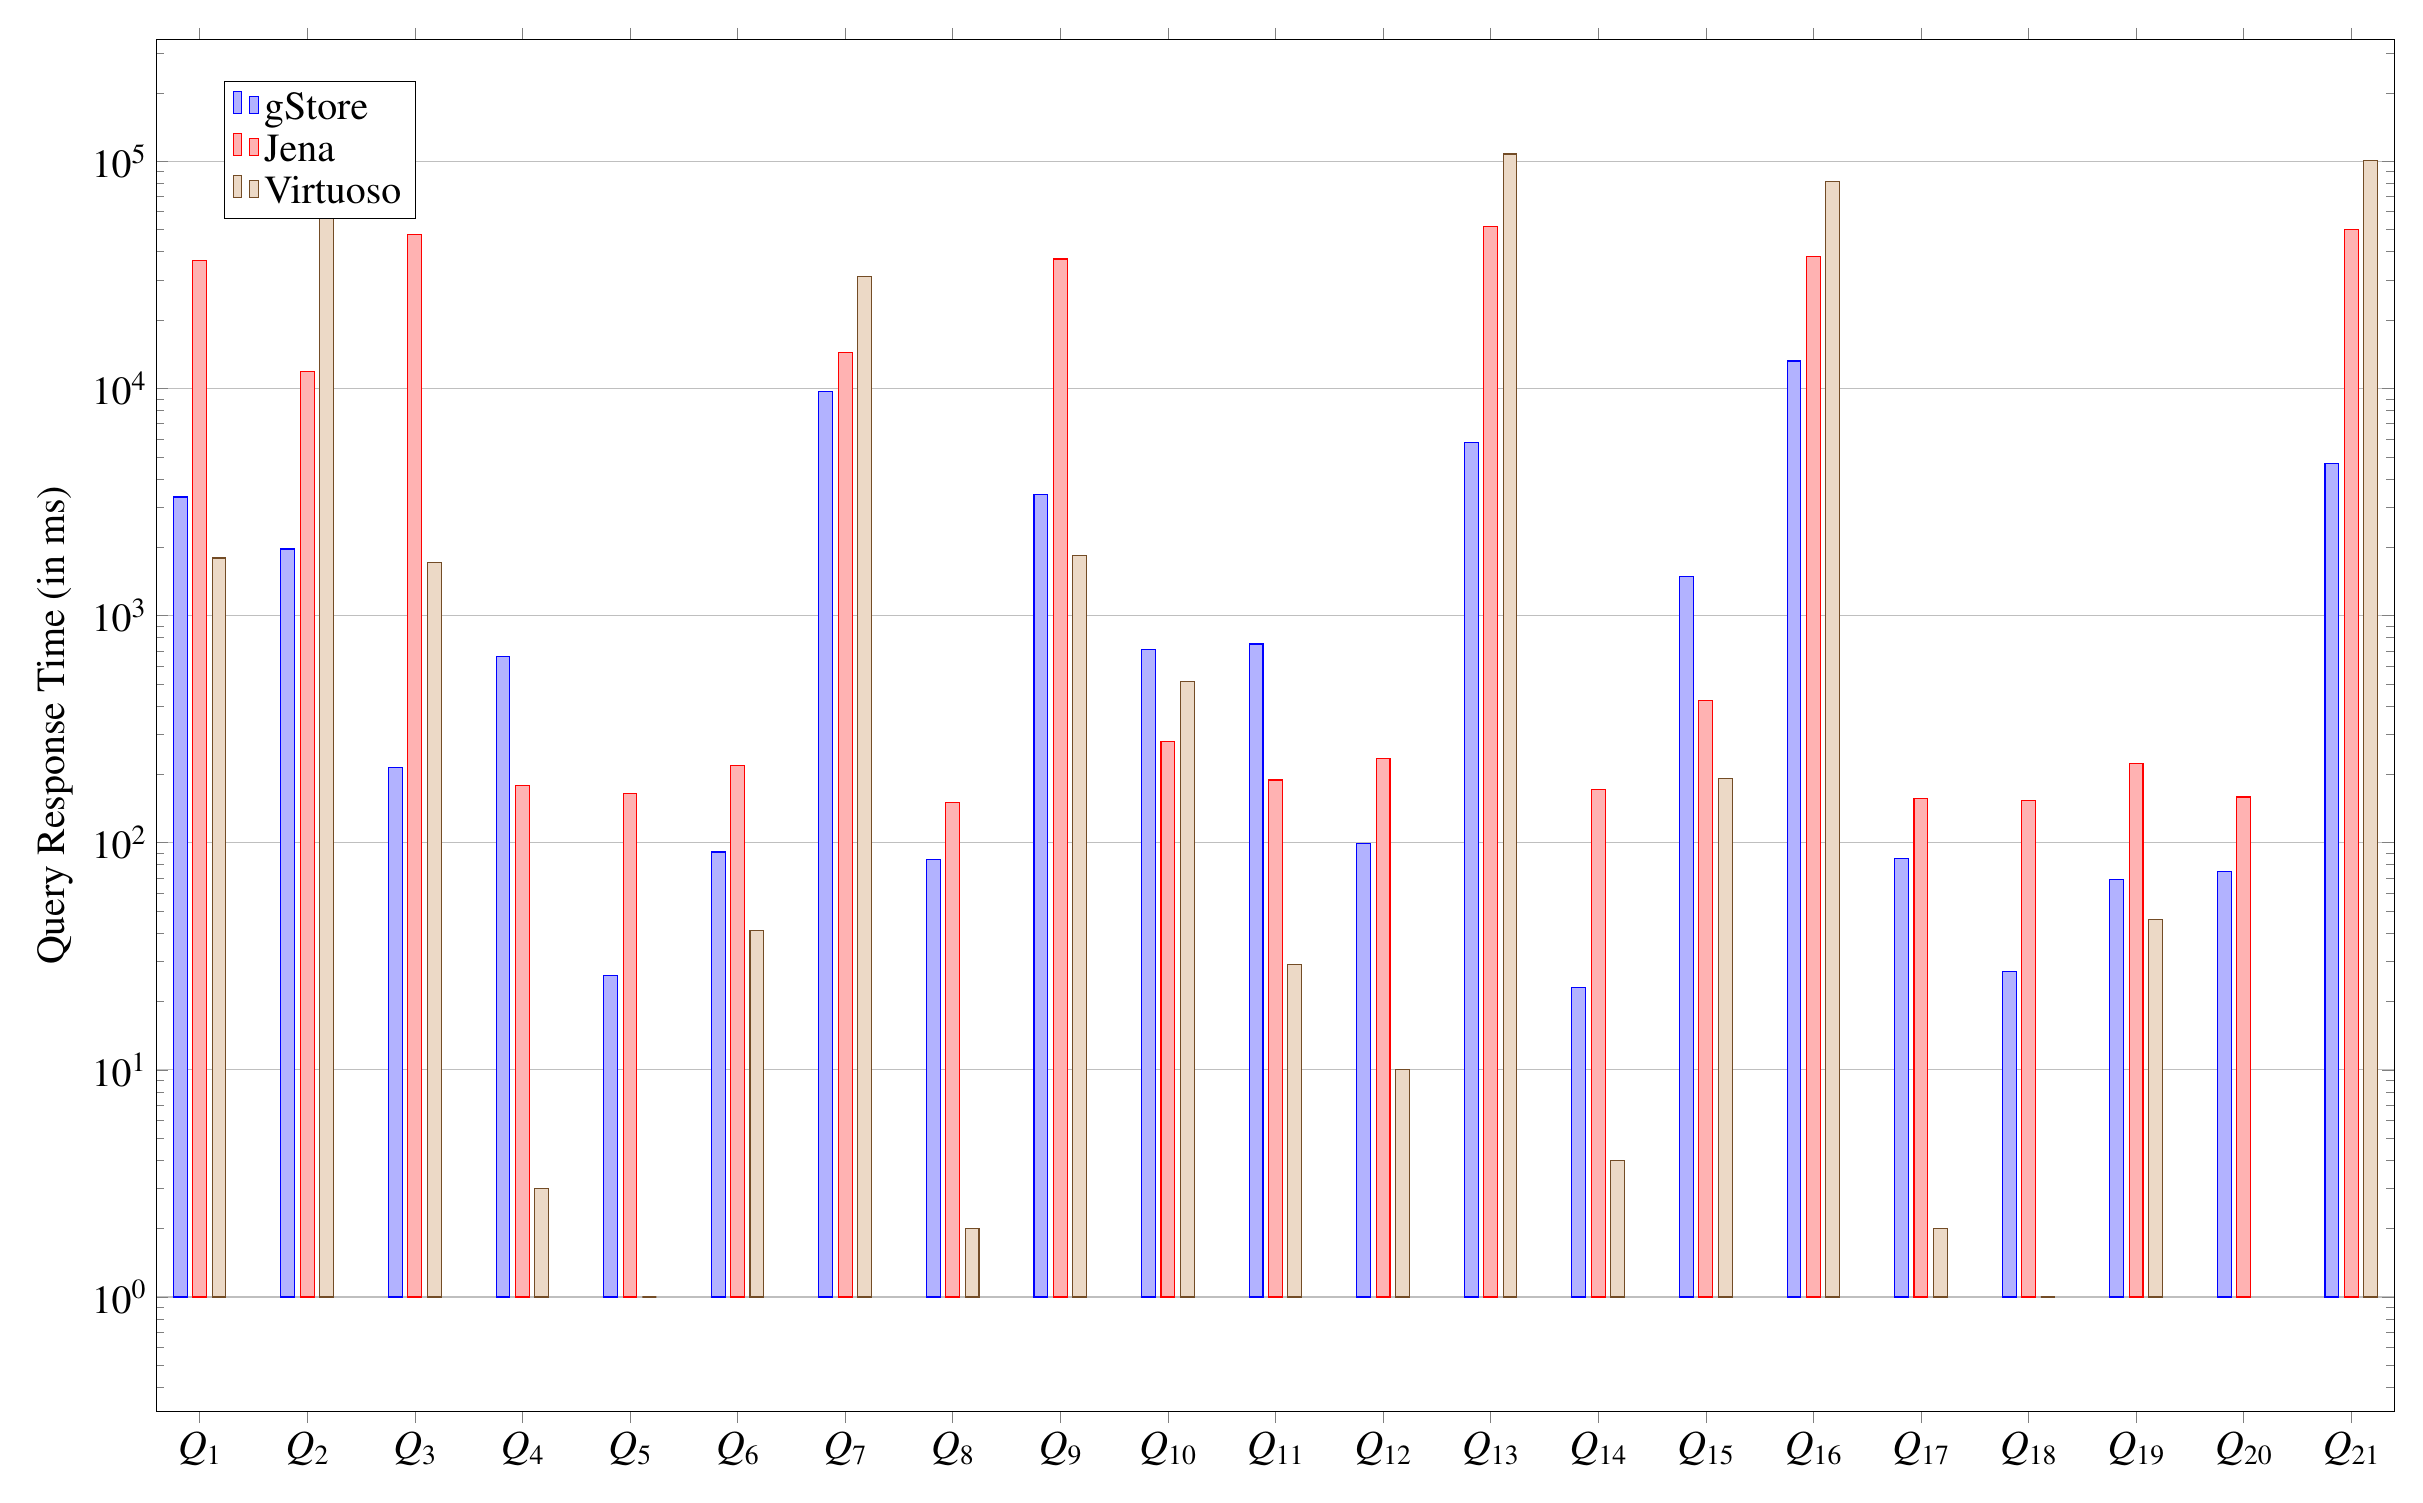
\begin{tikzpicture}[font=\Large]
 		 \begin{semilogyaxis}[
               width = 30cm,
               height = 19cm ,
    			ybar,
   			ymajorgrids = true,
   			ylabel = {Query Response Time (in ms)},
                %xlabel = {Queries},
    			symbolic x coords = 
    				{$Q_{1}$,$Q_{2}$,$Q_{3}$,$Q_{4}$,$Q_{5}$,$Q_{6}$,$Q_{7}$,$Q_{8}$,$Q_{9}$,$Q_{10}$,$Q_{11}$,$Q_{12}$,$Q_{13}$,$Q_{14}$,$Q_{15}$,$Q_{16}$,$Q_{17}$,$Q_{18}$,$Q_{19}$,$Q_{20}$,$Q_{21}$},
    bar width=5pt,
             enlarge x limits=0.02,
    			scaled y ticks = true,
			legend pos= north west,
 legend cell align=left
   		]
   \addplot coordinates {($Q_{1}$, 3328) ($Q_{2}$, 1965) ($Q_{3}$, 214) ($Q_{4}$, 661) ($Q_{5}$, 26) ($Q_{6}$, 91) ($Q_{7}$, 9692) ($Q_{8}$, 84) ($Q_{9}$, 3427) ($Q_{10}$, 707) ($Q_{11}$, 750) ($Q_{12}$, 99) ($Q_{13}$, 5796) ($Q_{14}$, 23) ($Q_{15}$, 1486) ($Q_{16}$, 13221) ($Q_{17}$, 85) ($Q_{18}$, 27) ($Q_{19}$, 69) ($Q_{20}$, 75) ($Q_{21}$, 4654)};
   
   
   \addplot coordinates {($Q_{1}$, 36694) ($Q_{2}$, 11859) ($Q_{3}$, 47511) ($Q_{4}$, 178) ($Q_{5}$, 164) ($Q_{6}$, 219) ($Q_{7}$, 14390) ($Q_{8}$, 151) ($Q_{9}$, 37158) ($Q_{10}$, 280) ($Q_{11}$, 189) ($Q_{12}$, 234) ($Q_{13}$, 51524) ($Q_{14}$, 172) ($Q_{15}$, 423) ($Q_{16}$, 37986) ($Q_{17}$, 156) ($Q_{18}$, 153) ($Q_{19}$, 224) ($Q_{20}$, 159) ($Q_{21}$, 49969)};
   
   \addplot coordinates {($Q_{1}$, 1793) ($Q_{2}$, 89629) ($Q_{3}$, 1711) ($Q_{4}$, 3) ($Q_{5}$, 1) ($Q_{6}$, 41) ($Q_{7}$, 31065) ($Q_{8}$, 2) ($Q_{9}$, 1846) ($Q_{10}$, 513) ($Q_{11}$, 29) ($Q_{12}$, 10) ($Q_{13}$, 107746) ($Q_{14}$, 4) ($Q_{15}$, 191) ($Q_{16}$, 81779) ($Q_{17}$, 2) ($Q_{18}$, 1) ($Q_{19}$, 46) ($Q_{20}$, 0) ($Q_{21}$, 100518)};
		
   		 \legend{gStore,Jena, Virtuoso}
  		\end{semilogyaxis}
\end{tikzpicture}

			}
			\label{fig:lubm200MPerformance}%
		}%
			\\
			\subfigure[lubm300M]{%
				\resizebox{\columnwidth}{!}{
						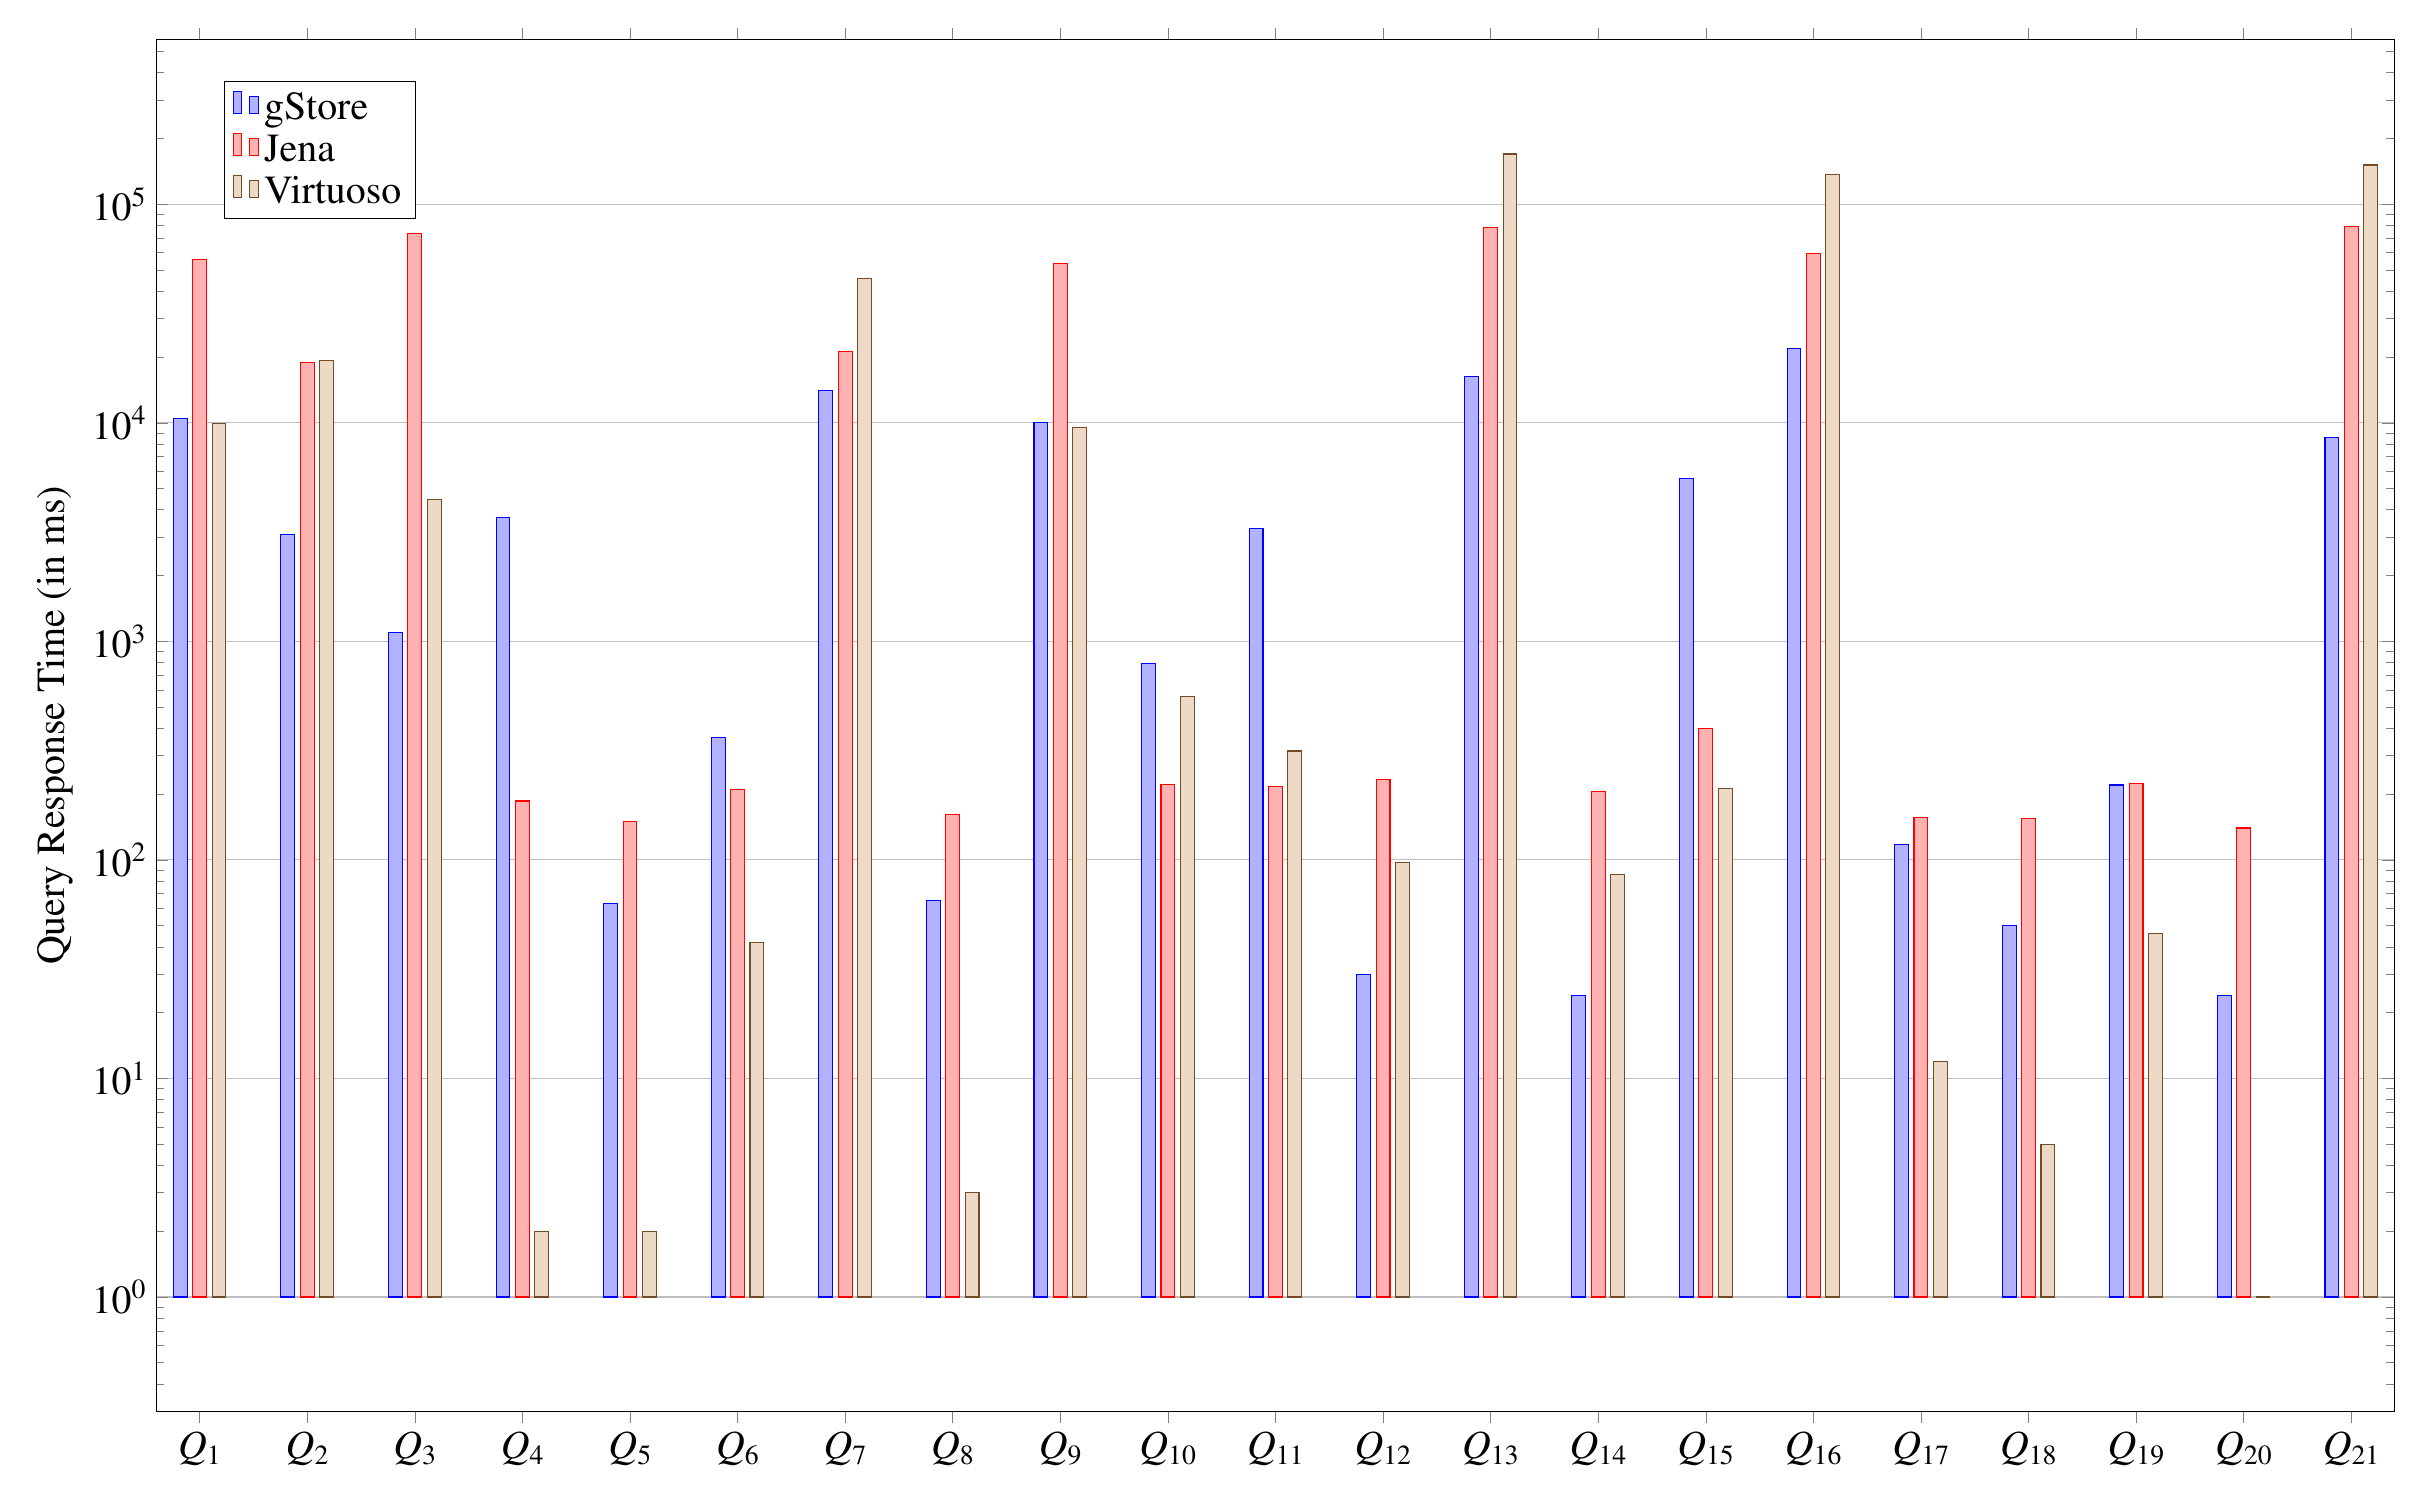
\begin{tikzpicture}[font=\Large]
 		 \begin{semilogyaxis}[
               width = 30cm,
               height = 19cm,
    			ybar,
   			ymajorgrids = true,
   			ylabel = {Query Response Time (in ms)},
                %xlabel = {Queries},
    			symbolic x coords = 
    				{$Q_{1}$,$Q_{2}$,$Q_{3}$,$Q_{4}$,$Q_{5}$,$Q_{6}$,$Q_{7}$,$Q_{8}$,$Q_{9}$,$Q_{10}$,$Q_{11}$,$Q_{12}$,$Q_{13}$,$Q_{14}$,$Q_{15}$,$Q_{16}$,$Q_{17}$,$Q_{18}$,$Q_{19}$,$Q_{20}$,$Q_{21}$},
    bar width=5pt,
             enlarge x limits=0.02,
    			scaled y ticks = true,
			legend pos= north west,
 legend cell align=left
   		]
   \addplot coordinates {($Q_{1}$, 10448) ($Q_{2}$, 3070) ($Q_{3}$, 1102) ($Q_{4}$, 3683) ($Q_{5}$, 63) ($Q_{6}$, 364) ($Q_{7}$, 14044) ($Q_{8}$, 65) ($Q_{9}$, 10075) ($Q_{10}$, 793) ($Q_{11}$, 3299) ($Q_{12}$, 30) ($Q_{13}$, 16283) ($Q_{14}$, 24) ($Q_{15}$, 5548) ($Q_{16}$, 21780) ($Q_{17}$, 118) ($Q_{18}$, 50) ($Q_{19}$, 220) ($Q_{20}$, 24) ($Q_{21}$, 8563)};
   
   
   \addplot coordinates {($Q_{1}$, 55647) ($Q_{2}$, 18903) ($Q_{3}$, 73675) ($Q_{4}$, 186) ($Q_{5}$, 150) ($Q_{6}$, 209) ($Q_{7}$, 21126) ($Q_{8}$, 161) ($Q_{9}$, 53551) ($Q_{10}$, 221) ($Q_{11}$, 217) ($Q_{12}$, 233) ($Q_{13}$, 77921) ($Q_{14}$, 205) ($Q_{15}$, 400) ($Q_{16}$, 59584) ($Q_{17}$, 156) ($Q_{18}$, 155) ($Q_{19}$, 224) ($Q_{20}$, 140) ($Q_{21}$, 79054)};
   
   \addplot coordinates {($Q_{1}$, 9930) ($Q_{2}$, 19241) ($Q_{3}$, 4471) ($Q_{4}$, 2) ($Q_{5}$, 2) ($Q_{6}$, 42) ($Q_{7}$, 45768) ($Q_{8}$, 3) ($Q_{9}$, 9523) ($Q_{10}$, 557) ($Q_{11}$, 315) ($Q_{12}$, 97) ($Q_{13}$, 169768) ($Q_{14}$, 86) ($Q_{15}$, 213) ($Q_{16}$, 137019) ($Q_{17}$, 12) ($Q_{18}$, 5) ($Q_{19}$, 46) ($Q_{20}$, 1) ($Q_{21}$, 151221)};
		
   		 \legend{gStore,Jena, Virtuoso}
  		\end{semilogyaxis}
\end{tikzpicture}

				}
				\label{fig:lubm300MPerformance}%
			}%
	\caption{Query Performance over LUBM 200M and 300M}%
	\label{fig:lubmPerformance2}
\end{figure}

\begin{figure}[t]%
	\subfigure[lubm500M]{%
		\resizebox{\columnwidth}{!}{
				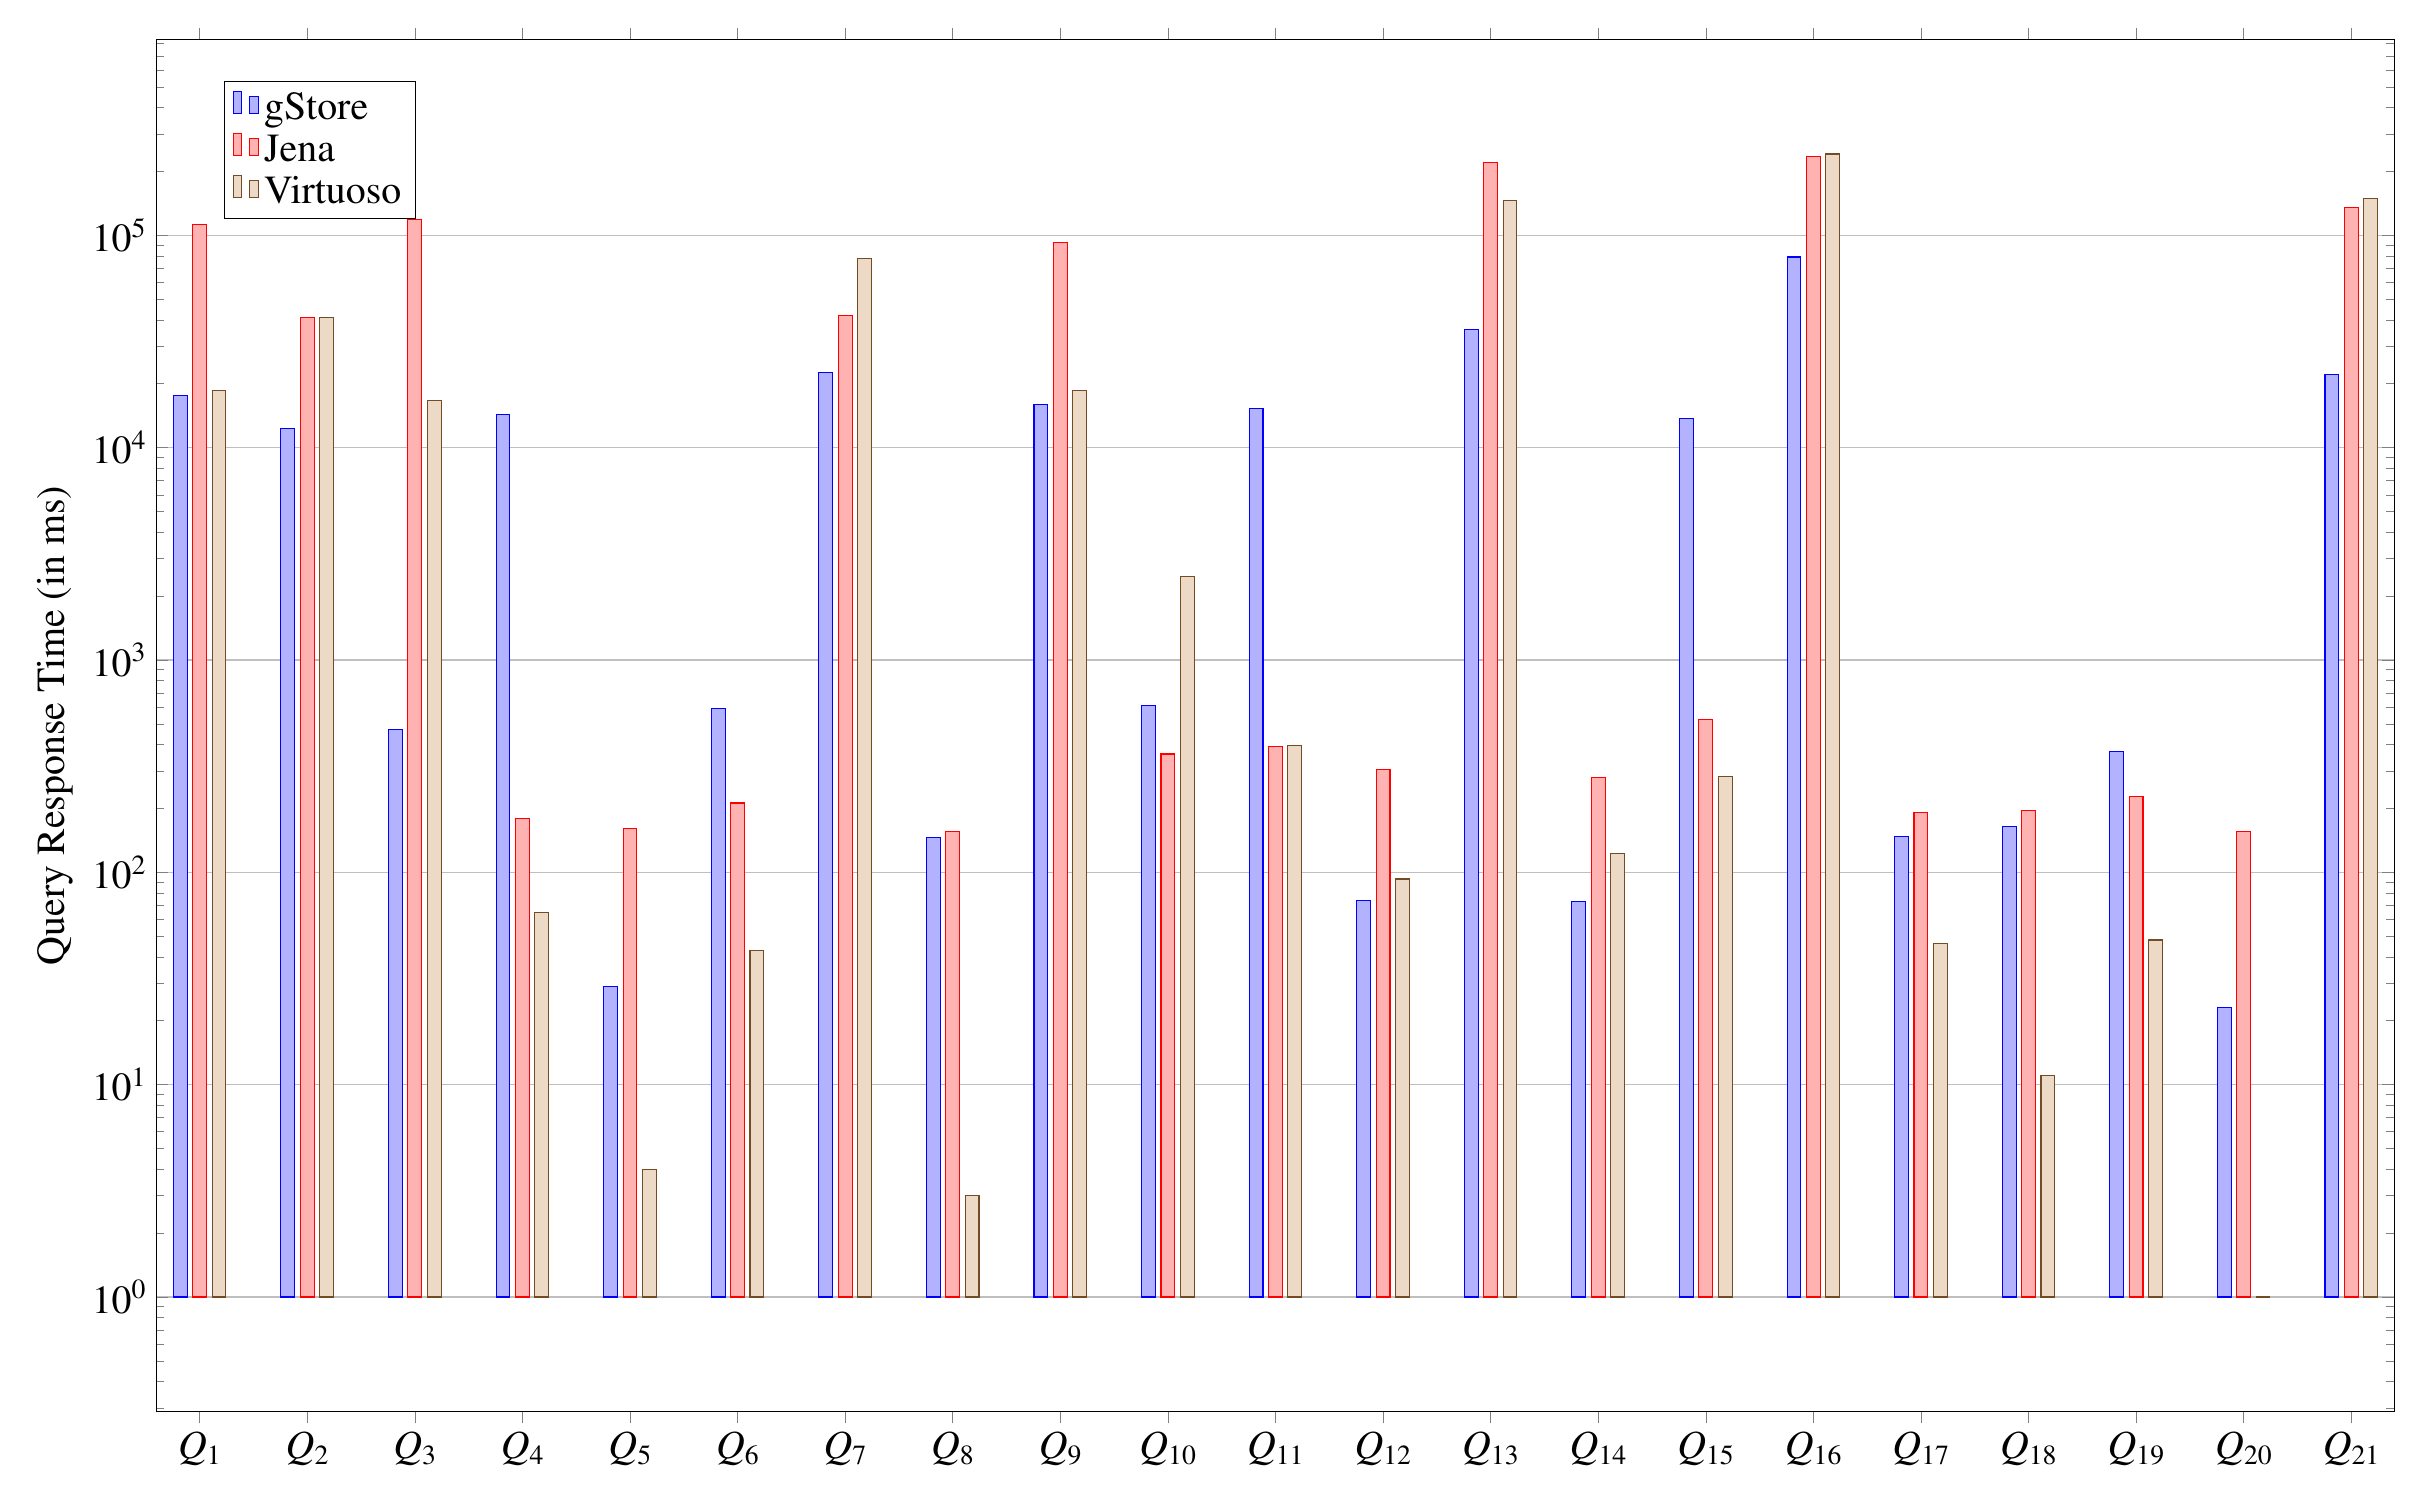
\begin{tikzpicture}[font=\Large]
 		 \begin{semilogyaxis}[
               width = 30cm,
               height = 19cm,
    			ybar,
   			ymajorgrids = true,
   			ylabel = {Query Response Time (in ms)},
                %xlabel = {Queries},
    			symbolic x coords = 
    				{$Q_{1}$,$Q_{2}$,$Q_{3}$,$Q_{4}$,$Q_{5}$,$Q_{6}$,$Q_{7}$,$Q_{8}$,$Q_{9}$,$Q_{10}$,$Q_{11}$,$Q_{12}$,$Q_{13}$,$Q_{14}$,$Q_{15}$,$Q_{16}$,$Q_{17}$,$Q_{18}$,$Q_{19}$,$Q_{20}$,$Q_{21}$},
    bar width=5pt,
             enlarge x limits=0.02,
    			scaled y ticks = true,
			legend pos= north west,
 legend cell align=left
   		]
   \addplot coordinates {($Q_{1}$, 17546) ($Q_{2}$, 12339) ($Q_{3}$, 470) ($Q_{4}$, 14382) ($Q_{5}$, 29) ($Q_{6}$, 592) ($Q_{7}$, 22611) ($Q_{8}$, 146) ($Q_{9}$, 15971) ($Q_{10}$, 609) ($Q_{11}$, 15353) ($Q_{12}$, 74) ($Q_{13}$, 36167) ($Q_{14}$, 73) ($Q_{15}$, 13718) ($Q_{16}$, 79076) ($Q_{17}$, 147) ($Q_{18}$, 164) ($Q_{19}$, 370) ($Q_{20}$, 23) ($Q_{21}$, 22039)};
   
    
    \addplot coordinates {($Q_{1}$, 112536) ($Q_{2}$, 40884) ($Q_{3}$, 119269) ($Q_{4}$, 180) ($Q_{5}$, 161) ($Q_{6}$, 212) ($Q_{7}$, 41979) ($Q_{8}$, 155) ($Q_{9}$, 92792) ($Q_{10}$, 361) ($Q_{11}$, 390) ($Q_{12}$, 305) ($Q_{13}$, 219391) ($Q_{14}$, 279) ($Q_{15}$, 526) ($Q_{16}$, 234164) ($Q_{17}$, 191) ($Q_{18}$, 195) ($Q_{19}$, 227) ($Q_{20}$, 155) ($Q_{21}$, 134847)};
    
    \addplot coordinates {($Q_{1}$, 18563) ($Q_{2}$, 40975) ($Q_{3}$, 16701) ($Q_{4}$, 65) ($Q_{5}$, 4) ($Q_{6}$, 43) ($Q_{7}$, 77484) ($Q_{8}$, 3) ($Q_{9}$, 18658) ($Q_{10}$, 2480) ($Q_{11}$, 397) ($Q_{12}$, 93) ($Q_{13}$, 145721) ($Q_{14}$, 123) ($Q_{15}$, 283) ($Q_{16}$, 241519) ($Q_{17}$, 46) ($Q_{18}$, 11) ($Q_{19}$, 48) ($Q_{20}$, 1) ($Q_{21}$, 148586)};
   		 \legend{gStore,Jena, Virtuoso}
  		\end{semilogyaxis}
\end{tikzpicture}

		}
		\label{fig:lubm500MPerformance}%
	}%
	\caption{Query Performance over LUBM 500M}%
	\label{fig:lubmPerformance3}
\end{figure}

\begin{figure}[t]%
	\subfigure[watdiv10M]{%
		\resizebox{\columnwidth}{!}{
				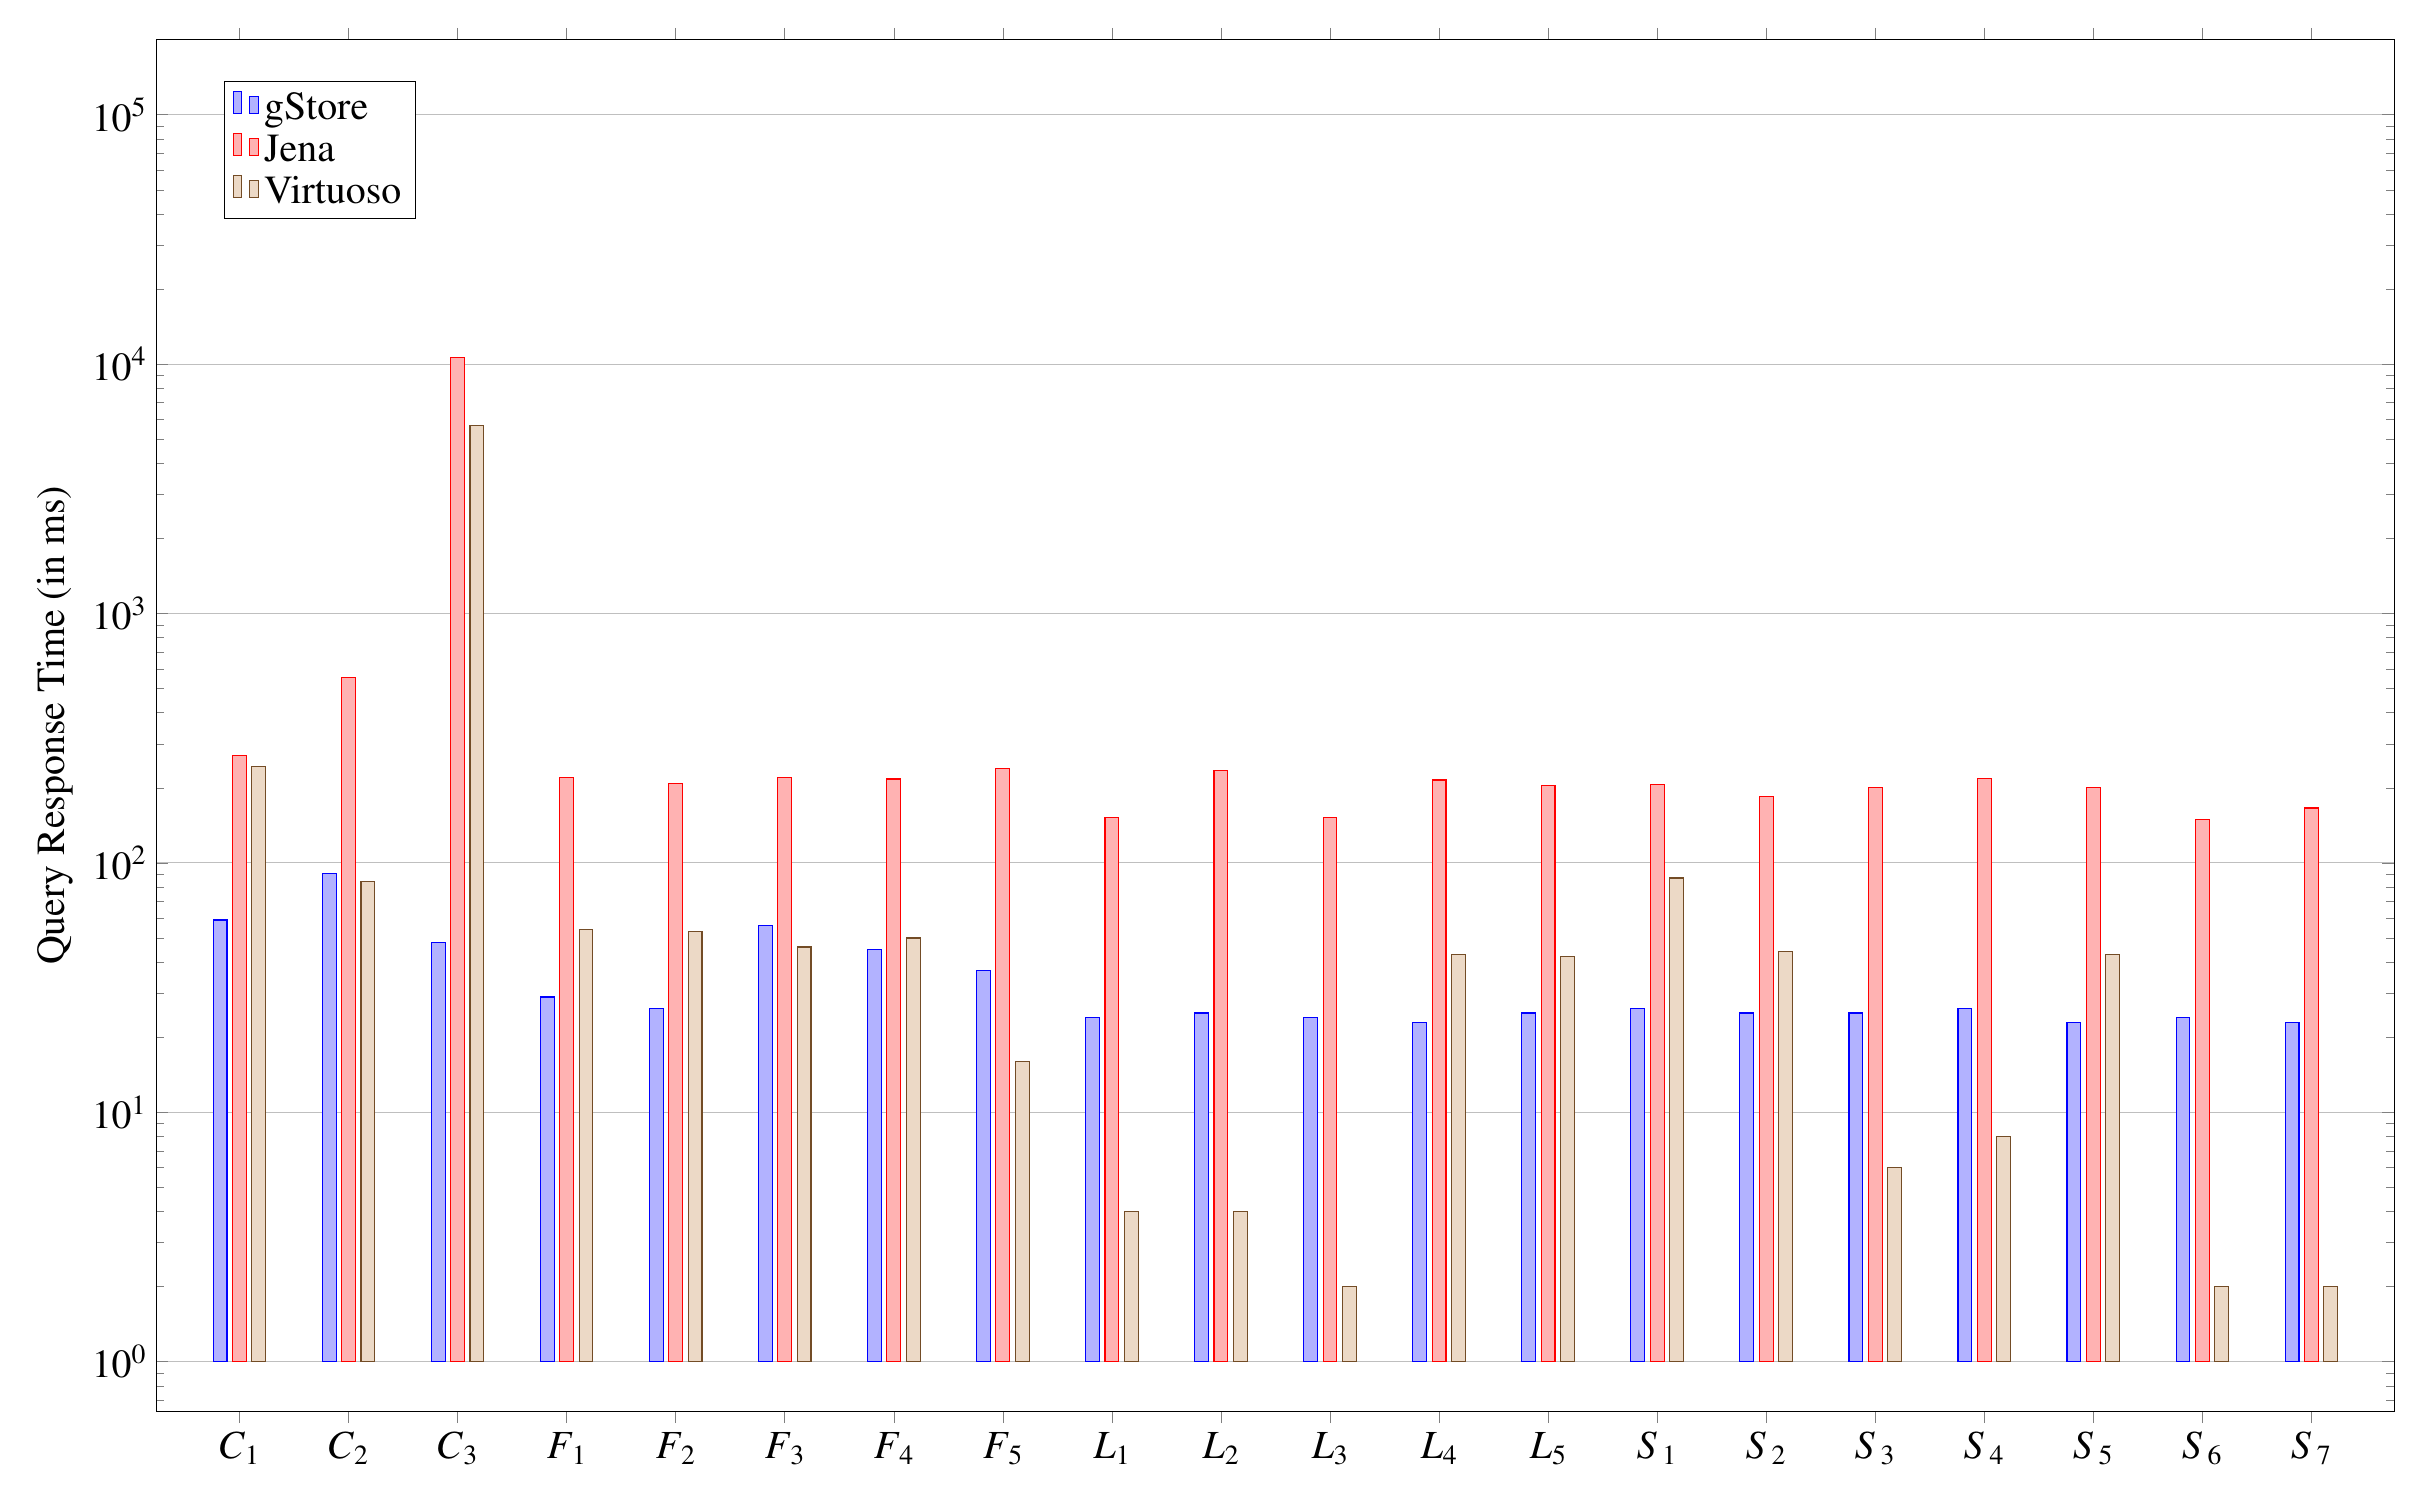
\begin{tikzpicture}[font=\Large]
 		 \begin{semilogyaxis}[
                width = 30cm,
               height = 19cm ,
               ymax=200000,
    			ybar,
   			ymajorgrids = true,
   			ylabel = {Query Response Time (in ms)},
                %xlabel = {Queries},
    			symbolic x coords = 
    			    			{$C_{1}$,$C_{2}$,$C_{3}$,$F_{1}$,$F_{2}$,$F_{3}$, $F_{4}$, $F_{5}$, $L_{1}$,$L_{2}$,$L_{3}$,$L_{4}$,$L_{5}$, $S_{1}$,$S_{2}$,$S_{3}$,$S_{4}$,$S_{5}$,$S_{6}$,$S_{7}$},
    bar width=5pt,
             enlarge x limits=0.04,
    			scaled y ticks = true,
			legend pos= north west,
 legend cell align=left
   		]
   		
   \addplot coordinates {($C_{1}$, 59) ($C_{2}$, 91) ($C_{3}$, 48) ($F_{1}$, 29) ($F_{2}$, 26) ($F_{3}$, 56) ($F_{4}$, 45) ($F_{5}$, 37) ($L_{1}$, 24) ($L_{2}$, 25) ($L_{3}$, 24) ($L_{4}$, 23) ($L_{5}$, 25) ($S_{1}$, 26) ($S_{2}$, 25) ($S_{3}$, 25) ($S_{4}$, 26) ($S_{5}$, 23) ($S_{6}$, 24) ($S_{7}$,23)};   
   
   \addplot coordinates {($C_{1}$, 270) ($C_{2}$, 556) ($C_{3}$, 10674) ($F_{1}$, 220) ($F_{2}$, 209) ($F_{3}$, 220) ($F_{4}$, 217) ($F_{5}$, 239) ($L_{1}$, 152) ($L_{2}$, 235) ($L_{3}$, 152) ($L_{4}$, 215) ($L_{5}$, 204) ($S_{1}$, 207) ($S_{2}$, 184) ($S_{3}$, 201) ($S_{4}$, 218) ($S_{5}$, 201) ($S_{6}$, 149) ($S_{7}$, 166)};   
   
   \addplot coordinates {($C_{1}$, 243) ($C_{2}$, 84) ($C_{3}$, 5663) ($F_{1}$, 54) ($F_{2}$, 53) ($F_{3}$, 46) ($F_{4}$, 50) ($F_{5}$, 16) ($L_{1}$, 4) ($L_{2}$, 4) ($L_{3}$, 2) ($L_{4}$, 43) ($L_{5}$, 42) ($S_{1}$, 87) ($S_{2}$, 44) ($S_{3}$, 6) ($S_{4}$, 8) ($S_{5}$, 43) ($S_{6}$, 2) ($S_{7}$, 2)};		
   
   		 \legend{gStore,Jena, Virtuoso}
  		\end{semilogyaxis}
\end{tikzpicture}

		}
		\label{fig:watdiv10MPerformance}%
	}%
	\\
	\subfigure[watdiv100M]{%
		\resizebox{\columnwidth}{!}{
				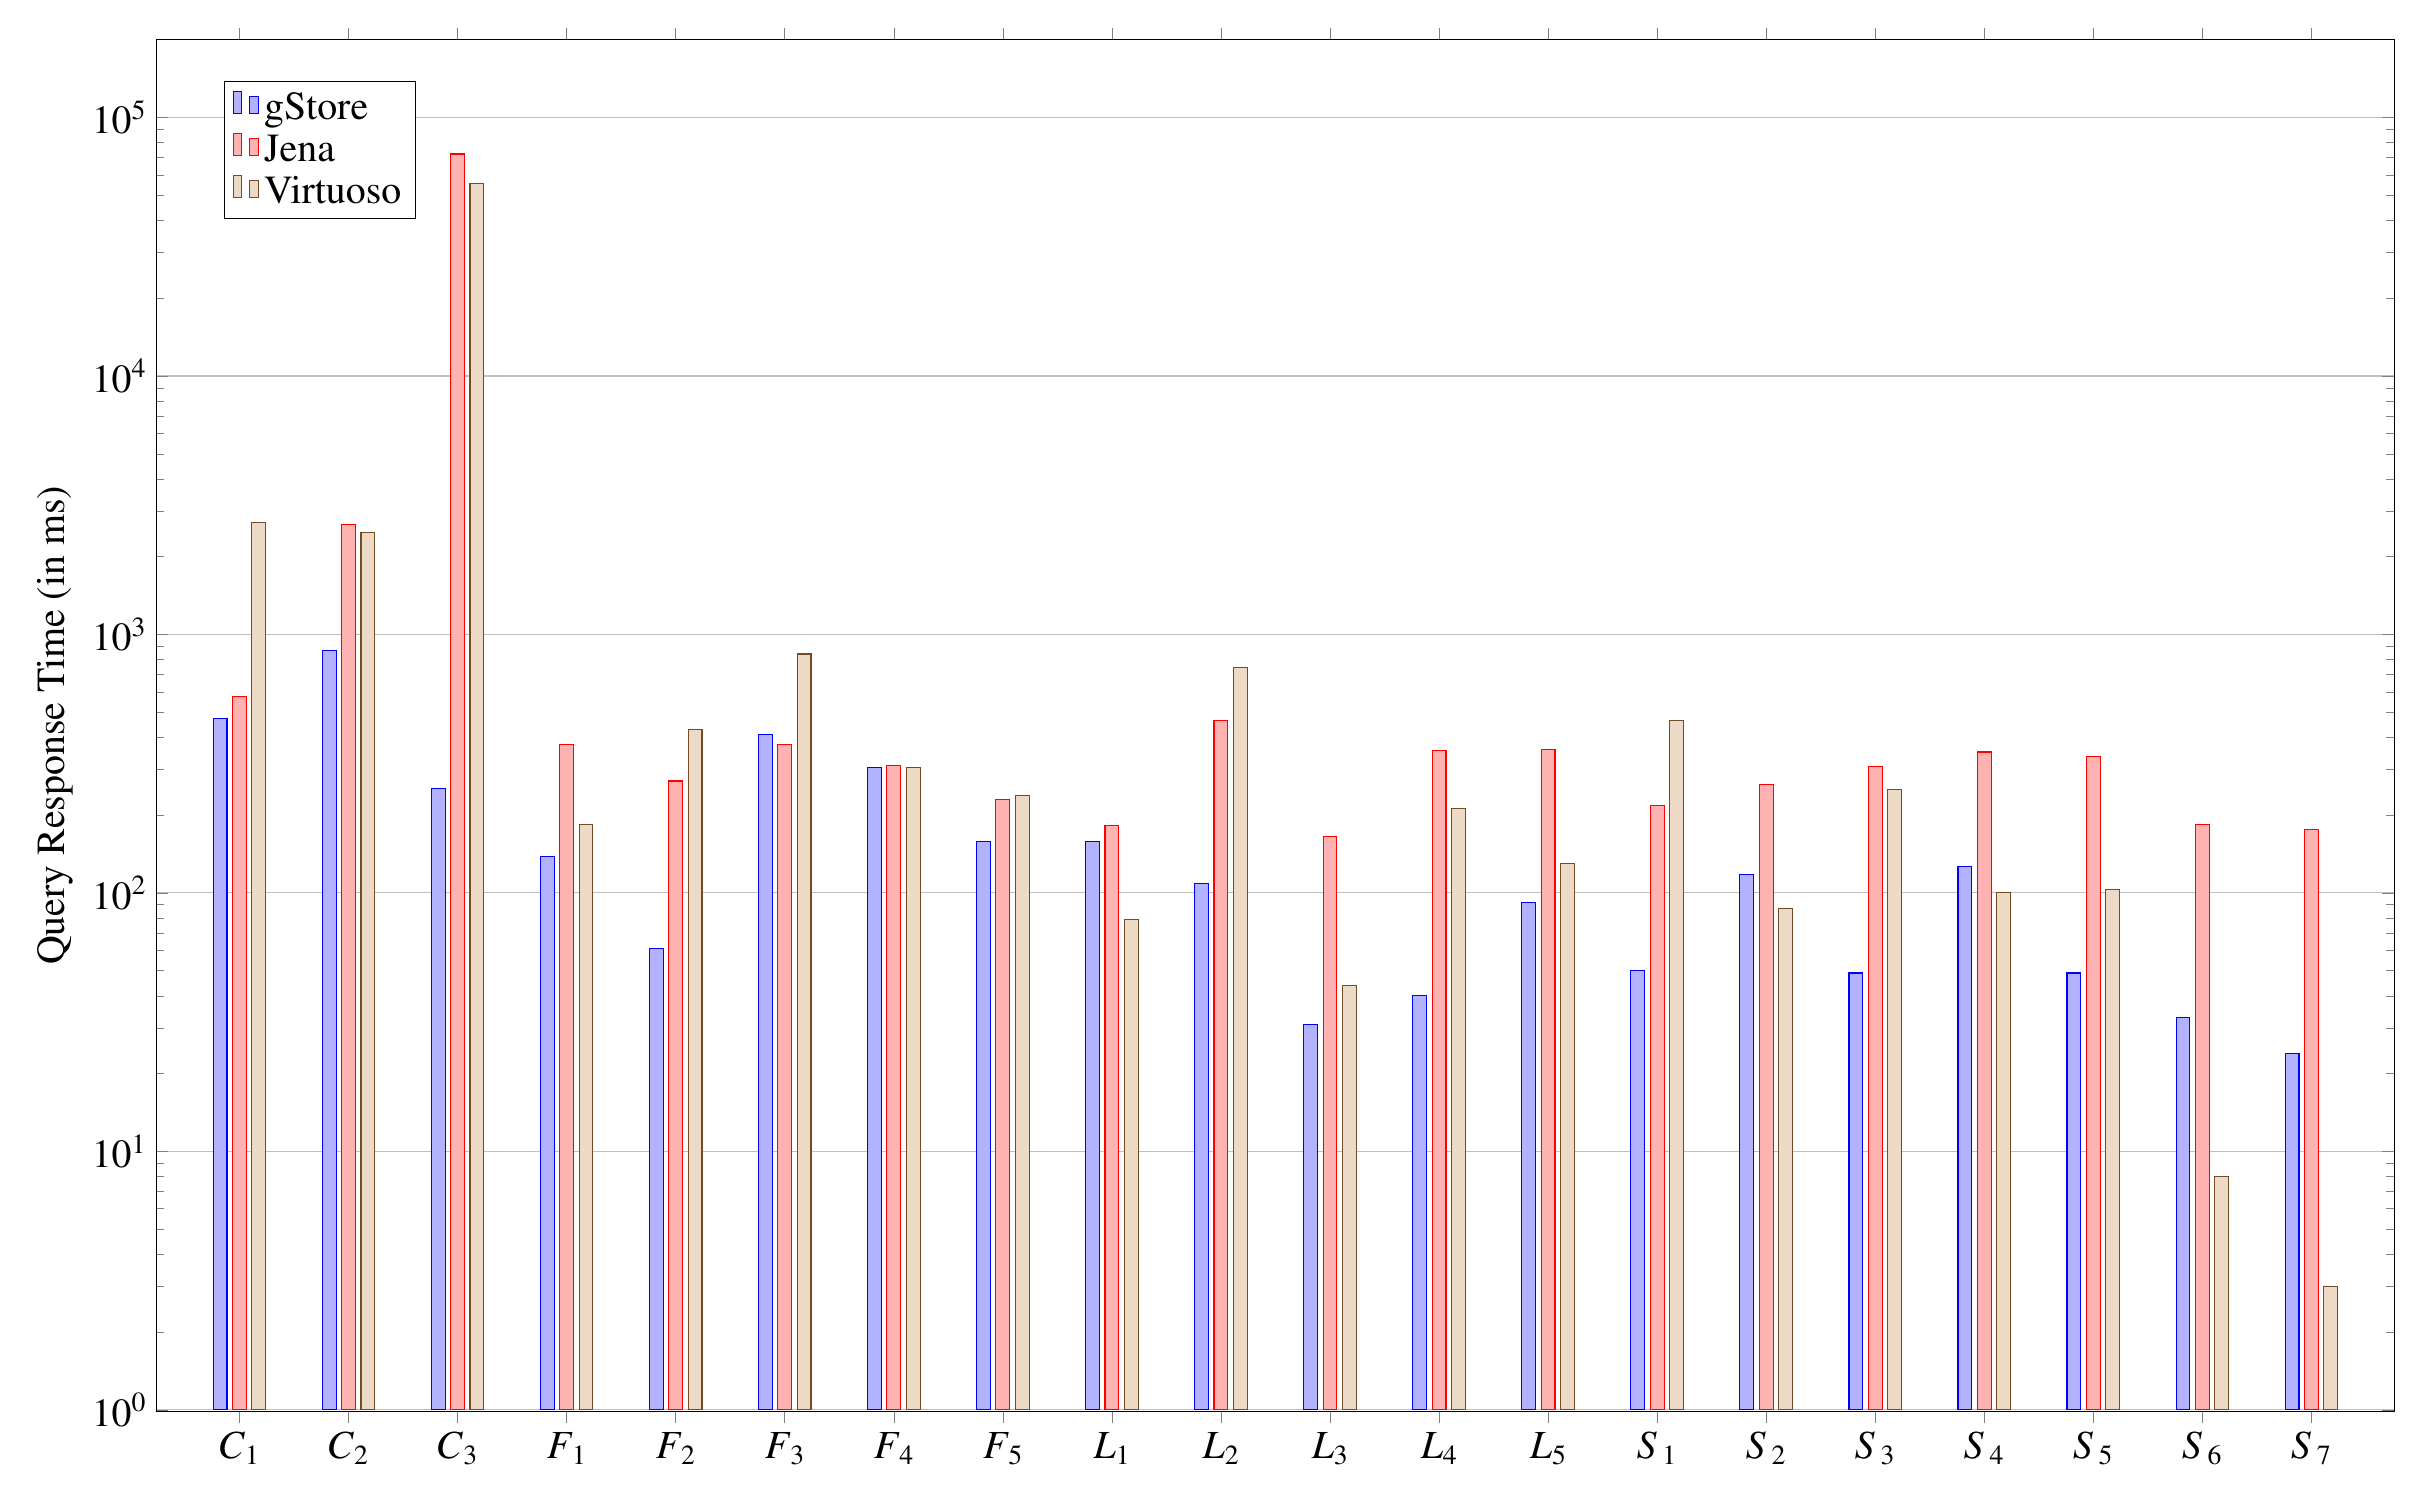
\begin{tikzpicture}[font=\Large]
 		 \begin{semilogyaxis}[
                width = 30cm,
               height = 19cm ,
               ymax=200000,
    			ybar,
   			ymajorgrids = true,
   			ylabel = {Query Response Time (in ms)},
                %xlabel = {Queries},
    			symbolic x coords = 
    			{$C_{1}$,$C_{2}$,$C_{3}$,$F_{1}$,$F_{2}$,$F_{3}$, $F_{4}$, $F_{5}$, $L_{1}$,$L_{2}$,$L_{3}$,$L_{4}$,$L_{5}$, $S_{1}$,$S_{2}$,$S_{3}$,$S_{4}$,$S_{5}$,$S_{6}$,$S_{7}$},
    bar width=5pt,
             enlarge x limits=0.04,
    			scaled y ticks = true,
			legend pos= north west,
 legend cell align=left
   		]

 \addplot coordinates {($C_{1}$, 472) ($C_{2}$, 865) ($C_{3}$, 254) ($F_{1}$, 138) ($F_{2}$, 61) ($F_{3}$, 410) ($F_{4}$, 305) ($F_{5}$, 158) ($L_{1}$, 158) ($L_{2}$, 109) ($L_{3}$, 31) ($L_{4}$, 40) ($L_{5}$, 92) ($S_{1}$, 50) ($S_{2}$, 118) ($S_{3}$, 49) ($S_{4}$, 127) ($S_{5}$, 49) ($S_{6}$, 33) ($S_{7}$, 24)};   
 
 \addplot coordinates {($C_{1}$, 577) ($C_{2}$, 2656) ($C_{3}$, 72280) ($F_{1}$, 375) ($F_{2}$, 271) ($F_{3}$, 374) ($F_{4}$, 312) ($F_{5}$, 230) ($L_{1}$, 183) ($L_{2}$, 465) ($L_{3}$, 165) ($L_{4}$, 357) ($L_{5}$, 358) ($S_{1}$, 218) ($S_{2}$, 262) ($S_{3}$, 308) ($S_{4}$, 351) ($S_{5}$, 337) ($S_{6}$, 184) ($S_{7}$, 176)};   
 
 \addplot coordinates {($C_{1}$, 2718) ($C_{2}$, 2477) ($C_{3}$, 55463) ($F_{1}$, 184) ($F_{2}$, 430) ($F_{3}$, 840) ($F_{4}$, 305) ($F_{5}$, 238) ($L_{1}$, 79) ($L_{2}$, 748) ($L_{3}$, 44) ($L_{4}$, 213) ($L_{5}$, 130) ($S_{1}$, 466) ($S_{2}$, 87) ($S_{3}$, 252) ($S_{4}$, 100) ($S_{5}$, 103) ($S_{6}$, 8) ($S_{7}$, 3)};		

   		 \legend{gStore,Jena, Virtuoso}
  		\end{semilogyaxis}
\end{tikzpicture}

		}
		\label{fig:watdiv100MPerformance}%
	}%
	\caption{Query Performance over WatDiv 10M and 100M}%
	\label{fig:watdivPerformance1}
\end{figure}
	
	\begin{figure}[t]%
	\subfigure[watdiv200M]{%
		\resizebox{\columnwidth}{!}{
				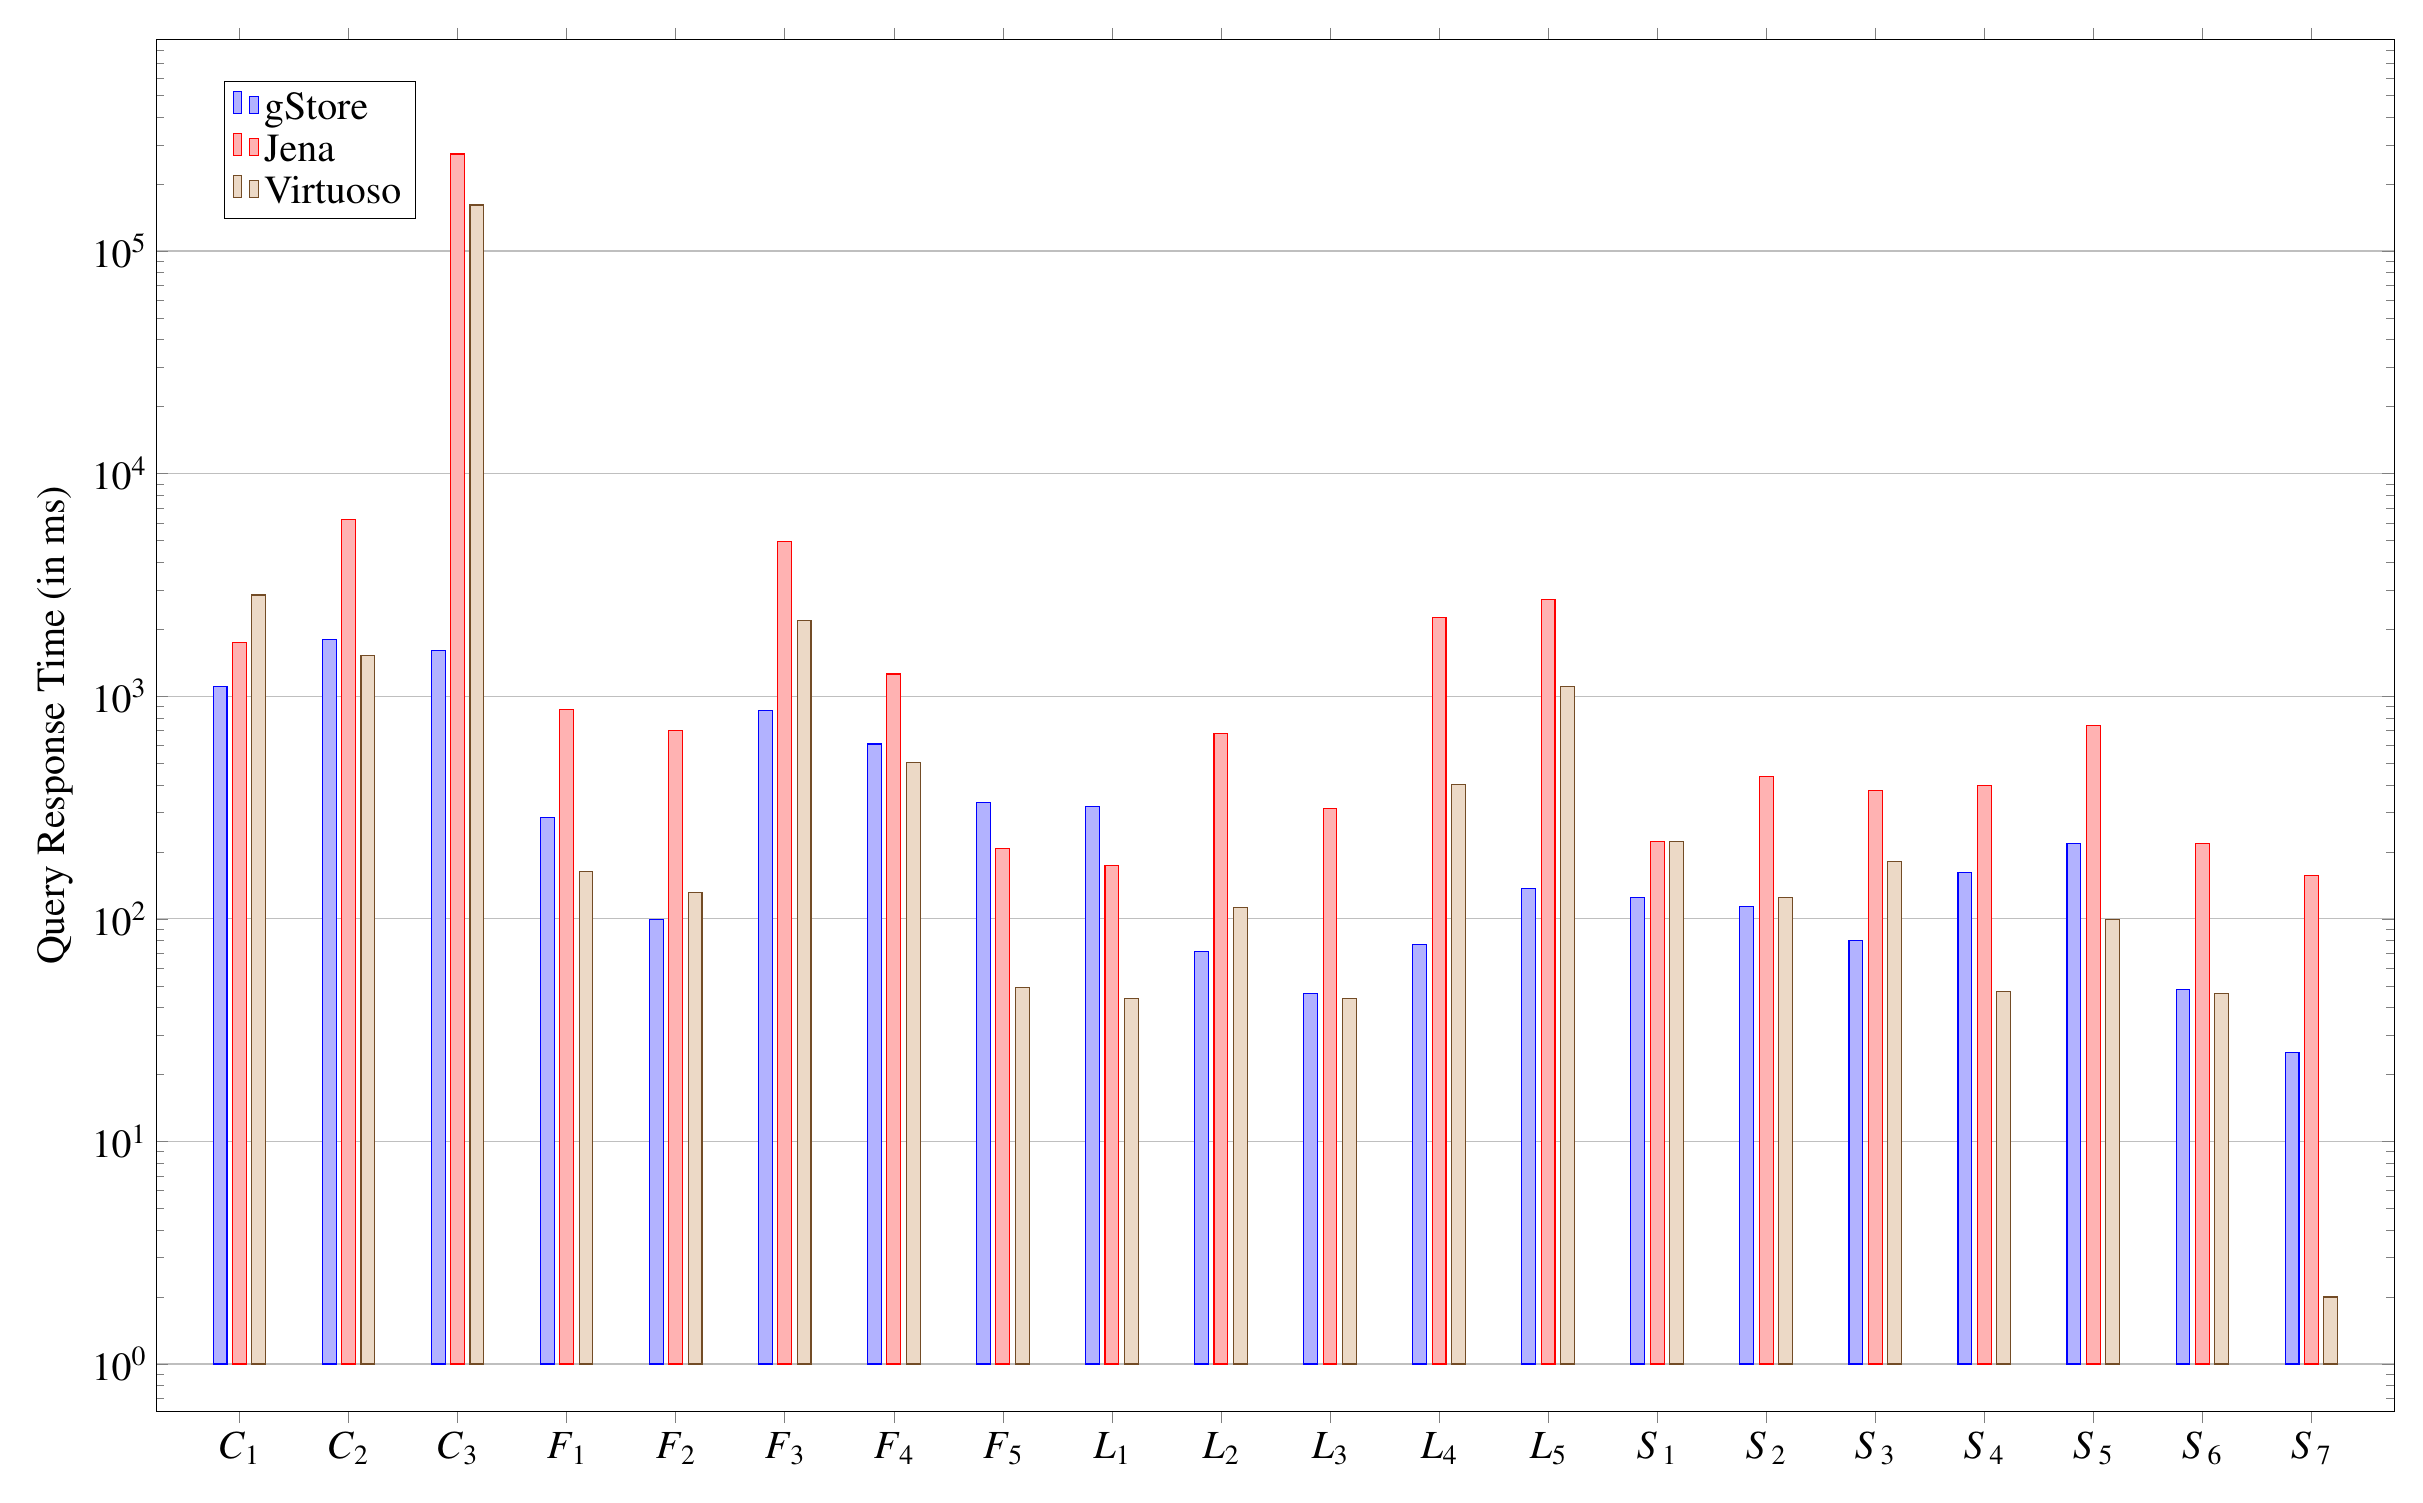
\begin{tikzpicture}[font=\Large]
 		 \begin{semilogyaxis}[
                width = 30cm,
               height = 19cm ,
    			ybar,
   			ymajorgrids = true,
   			ylabel = {Query Response Time (in ms)},
                %xlabel = {Queries},
    			symbolic x coords = 
    			    			{$C_{1}$,$C_{2}$,$C_{3}$,$F_{1}$,$F_{2}$,$F_{3}$, $F_{4}$, $F_{5}$, $L_{1}$,$L_{2}$,$L_{3}$,$L_{4}$,$L_{5}$, $S_{1}$,$S_{2}$,$S_{3}$,$S_{4}$,$S_{5}$,$S_{6}$,$S_{7}$},
    bar width=5pt,
             enlarge x limits=0.04,
    			scaled y ticks = true,
			legend pos= north west,
 legend cell align=left
   		]

   \addplot coordinates {($C_{1}$, 1103) ($C_{2}$, 1804) ($C_{3}$, 1598) ($F_{1}$, 286) ($F_{2}$, 99) ($F_{3}$, 862) ($F_{4}$, 610) ($F_{5}$, 334) ($L_{1}$, 319) ($L_{2}$, 71) ($L_{3}$, 46) ($L_{4}$, 77) ($L_{5}$, 137) ($S_{1}$, 125) ($S_{2}$, 114) ($S_{3}$, 80) ($S_{4}$, 161) ($S_{5}$, 217) ($S_{6}$, 48) ($S_{7}$, 25)};   
   
   \addplot coordinates {($C_{1}$, 1749) ($C_{2}$, 6242) ($C_{3}$, 272768) ($F_{1}$, 870) ($F_{2}$, 703) ($F_{3}$, 4975) ($F_{4}$, 1259) ($F_{5}$, 206) ($L_{1}$, 173) ($L_{2}$, 679) ($L_{3}$, 314) ($L_{4}$, 2256) ($L_{5}$, 2726) ($S_{1}$, 222) ($S_{2}$, 435) ($S_{3}$, 378) ($S_{4}$, 397) ($S_{5}$, 740) ($S_{6}$, 218) ($S_{7}$, 157)};   
   
   \addplot coordinates {($C_{1}$, 2850) ($C_{2}$, 1517) ($C_{3}$, 160982) ($F_{1}$, 163) ($F_{2}$, 131) ($F_{3}$, 2189) ($F_{4}$, 503) ($F_{5}$, 49) ($L_{1}$, 44) ($L_{2}$, 112) ($L_{3}$, 44) ($L_{4}$, 403) ($L_{5}$, 1102) ($S_{1}$, 223) ($S_{2}$, 125) ($S_{3}$, 181) ($S_{4}$, 47) ($S_{5}$, 99) ($S_{6}$, 46) ($S_{7}$, 2)};	
   
   		 \legend{gStore,Jena, Virtuoso}
  		\end{semilogyaxis}
\end{tikzpicture}

		}
		\label{fig:watdiv200MPerformance}%
	}%
	\\
	\subfigure[watdiv300M]{%
		\resizebox{\columnwidth}{!}{
				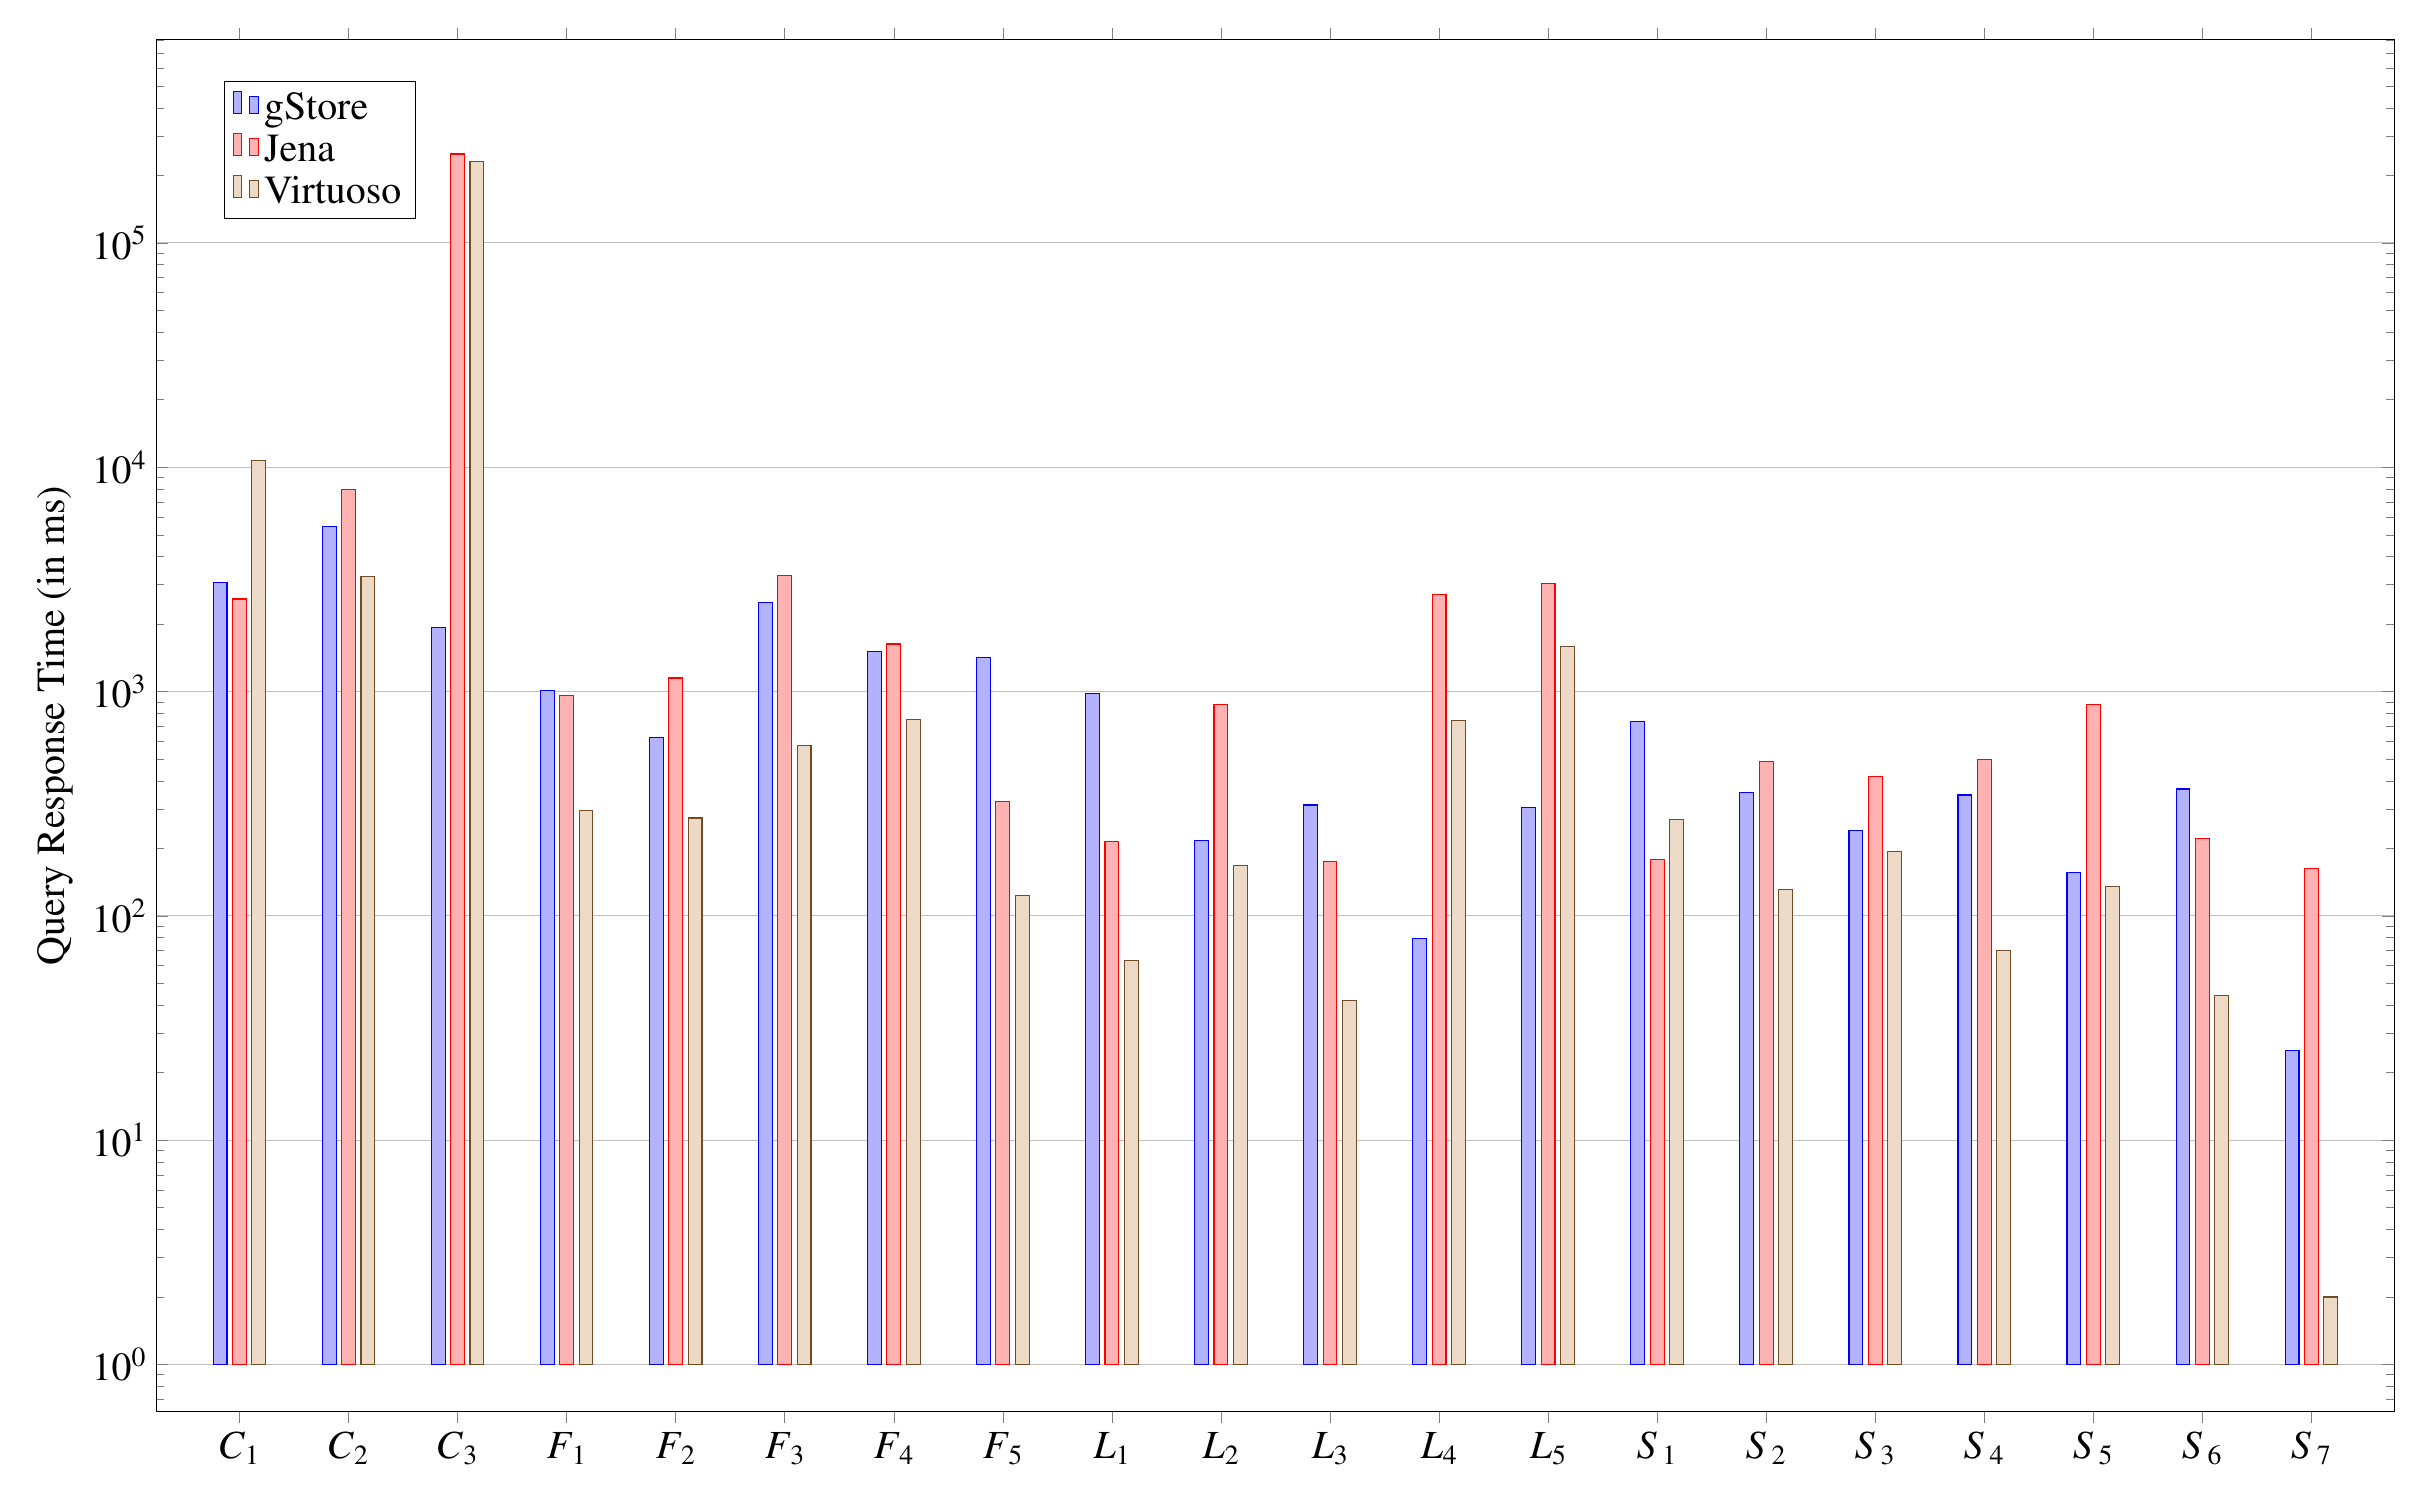
\begin{tikzpicture}[font=\Large]
 		 \begin{semilogyaxis}[
                width = 30cm,
               height = 19cm,
    			ybar,
   			ymajorgrids = true,
   			ylabel = {Query Response Time (in ms)},
                %xlabel = {Queries},
    			symbolic x coords = 
    			    	{$C_{1}$,$C_{2}$,$C_{3}$,$F_{1}$,$F_{2}$,$F_{3}$, $F_{4}$, $F_{5}$, $L_{1}$,$L_{2}$,$L_{3}$,$L_{4}$,$L_{5}$, $S_{1}$,$S_{2}$,$S_{3}$,$S_{4}$,$S_{5}$,$S_{6}$,$S_{7}$},
    bar width=5pt,
             enlarge x limits=0.04,
    			scaled y ticks = true,
			legend pos= north west,
 legend cell align=left
   		]
	  
	   \addplot coordinates {($C_{1}$, 3061) ($C_{2}$, 5421) ($C_{3}$, 1930) ($F_{1}$, 1014) ($F_{2}$, 626) ($F_{3}$, 2487) ($F_{4}$, 1505) ($F_{5}$, 1425) ($L_{1}$, 979) ($L_{2}$, 216) ($L_{3}$, 312) ($L_{4}$, 79) ($L_{5}$, 304) ($S_{1}$, 738) ($S_{2}$, 354) ($S_{3}$, 240) ($S_{4}$, 346) ($S_{5}$, 156) ($S_{6}$, 368) ($S_{7}$, 25)};   
	   
	   \addplot coordinates {($C_{1}$, 2587) ($C_{2}$, 7949) ($C_{3}$, 249066) ($F_{1}$, 958) ($F_{2}$, 1150) ($F_{3}$, 3306) ($F_{4}$, 1630) ($F_{5}$, 323) ($L_{1}$, 214) ($L_{2}$, 874) ($L_{3}$, 175) ($L_{4}$, 2721) ($L_{5}$, 3044) ($S_{1}$, 178) ($S_{2}$, 488) ($S_{3}$, 420) ($S_{4}$, 497) ($S_{5}$, 877) ($S_{6}$, 222) ($S_{7}$, 163)};   
	   
	   \addplot coordinates {($C_{1}$, 10706) ($C_{2}$, 3249) ($C_{3}$, 231171) ($F_{1}$, 296) ($F_{2}$, 273) ($F_{3}$, 573) ($F_{4}$, 748) ($F_{5}$, 123) ($L_{1}$, 63) ($L_{2}$, 168) ($L_{3}$, 42) ($L_{4}$, 744) ($L_{5}$, 1587) ($S_{1}$, 268) ($S_{2}$, 131) ($S_{3}$, 194) ($S_{4}$, 70) ($S_{5}$, 135) ($S_{6}$, 44) ($S_{7}$, 2)};		
	  		
   		 \legend{gStore,Jena,Virtuoso}
  		\end{semilogyaxis}
\end{tikzpicture}

		}
		\label{fig:watdiv300MPerformance}%
	}%
	\caption{Query Performance over WatDiv 200M and 300M}%
	\label{fig:watdivPerformance2}
\end{figure}

\begin{figure}[t]%
	\subfigure[watdiv500M]{%
		\resizebox{\columnwidth}{!}{
				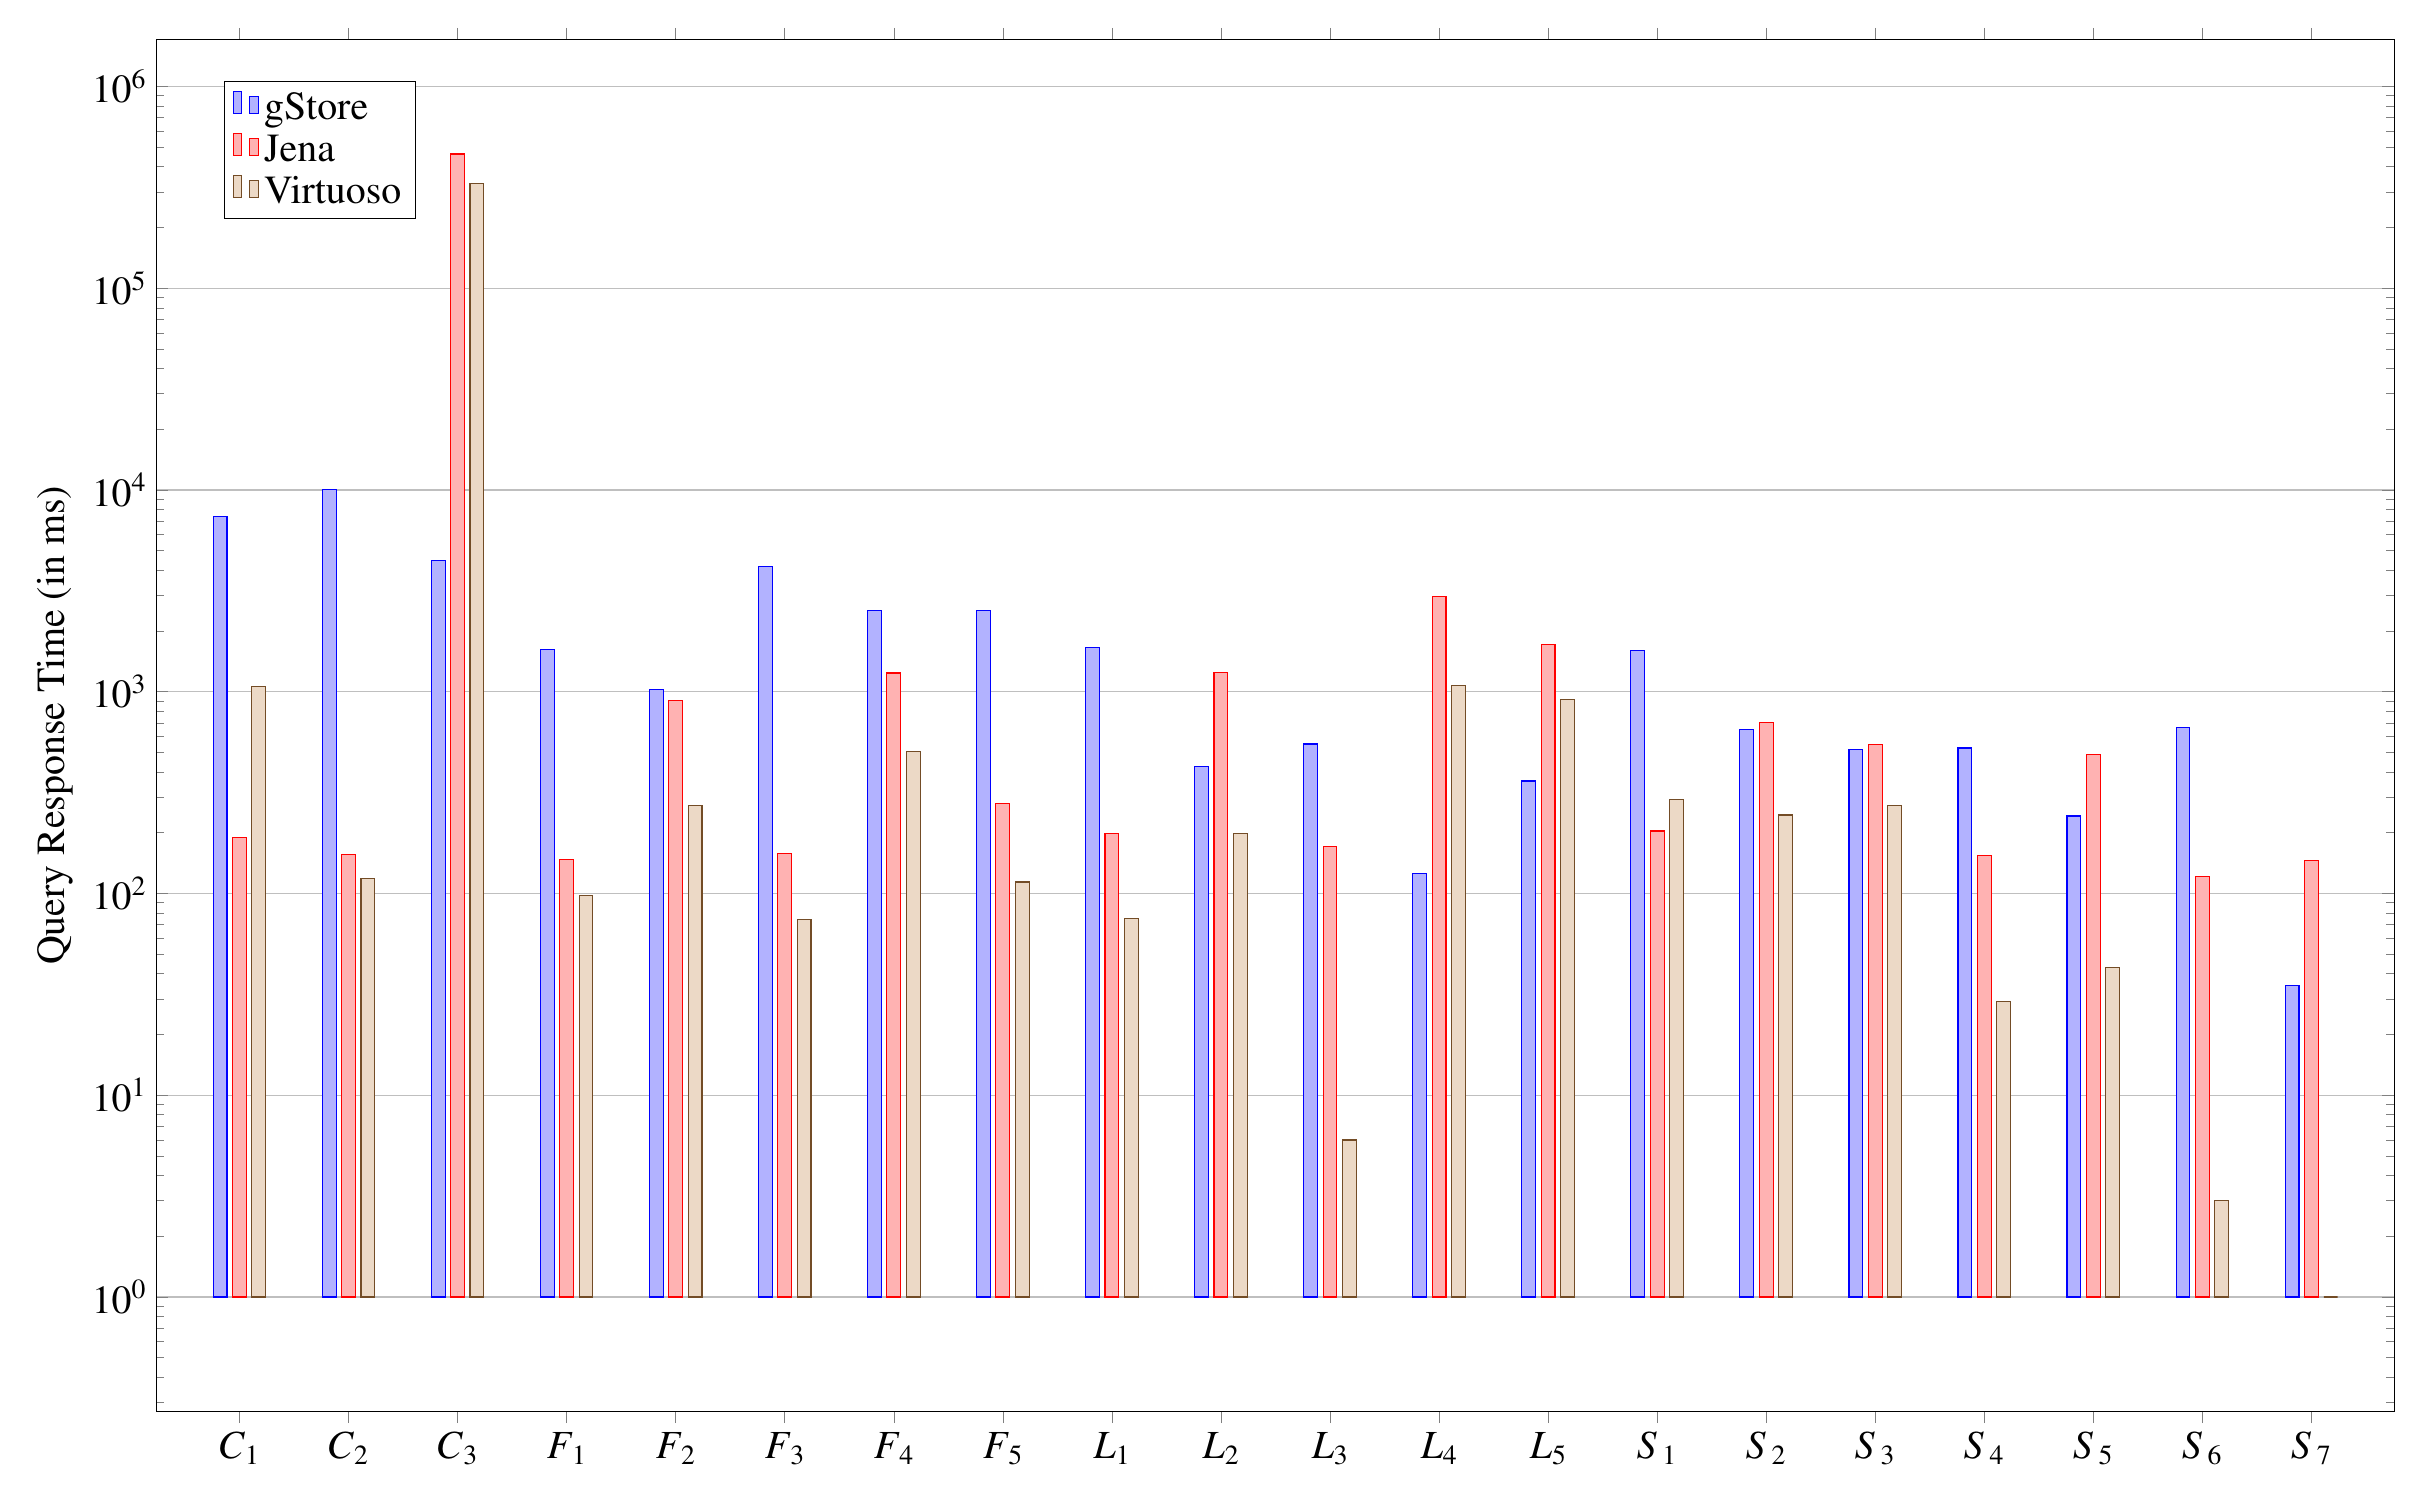
\begin{tikzpicture}[font=\Large]
 		 \begin{semilogyaxis}[
                width = 30cm,
               height = 19cm,
    			ybar,
   			ymajorgrids = true,
   			ylabel = {Query Response Time (in ms)},
                %xlabel = {Queries},
    			symbolic x coords = 
    			    	{$C_{1}$,$C_{2}$,$C_{3}$,$F_{1}$,$F_{2}$,$F_{3}$, $F_{4}$, $F_{5}$, $L_{1}$,$L_{2}$,$L_{3}$,$L_{4}$,$L_{5}$, $S_{1}$,$S_{2}$,$S_{3}$,$S_{4}$,$S_{5}$,$S_{6}$,$S_{7}$},
    bar width=5pt,
             enlarge x limits=0.04,
    			scaled y ticks = true,
			legend pos= north west,
 legend cell align=left
   		]
	  %\part{title}
	   \addplot coordinates {($C_{1}$, 7398) ($C_{2}$, 10036) ($C_{3}$, 4455) ($F_{1}$, 1616) ($F_{2}$, 1028) ($F_{3}$, 4188) ($F_{4}$, 2533) ($F_{5}$, 2533) ($L_{1}$, 1665) ($L_{2}$, 424) ($L_{3}$, 551) ($L_{4}$, 126) ($L_{5}$, 361) ($S_{1}$, 1608) ($S_{2}$, 650) ($S_{3}$, 518) ($S_{4}$, 526) ($S_{5}$, 242) ($S_{6}$, 668) ($S_{7}$, 35)};   
	   
	   \addplot coordinates {($C_{1}$, 189) ($C_{2}$, 156) ($C_{3}$, 462742) ($F_{1}$, 148) ($F_{2}$, 902) ($F_{3}$, 158) ($F_{4}$, 1239) ($F_{5}$, 280) ($L_{1}$, 198) ($L_{2}$, 1248) ($L_{3}$, 171) ($L_{4}$, 2965) ($L_{5}$, 1717) ($S_{1}$, 204) ($S_{2}$, 706) ($S_{3}$, 547) ($S_{4}$, 155) ($S_{5}$, 489) ($S_{6}$, 121) ($S_{7}$, 145)};   
	   
	   \addplot coordinates {($C_{1}$, 1066) ($C_{2}$, 119) ($C_{3}$, 331799) ($F_{1}$, 98) ($F_{2}$, 273) ($F_{3}$, 74) ($F_{4}$, 506) ($F_{5}$, 114) ($L_{1}$, 75) ($L_{2}$, 199) ($L_{3}$, 6) ($L_{4}$, 1069) ($L_{5}$, 919) ($S_{1}$, 293) ($S_{2}$, 245) ($S_{3}$, 274) ($S_{4}$, 29) ($S_{5}$, 43) ($S_{6}$, 3) ($S_{7}$, 1)};		
	  		
   		 \legend{gStore,Jena,Virtuoso}
  		\end{semilogyaxis}
\end{tikzpicture}

		}
		\label{fig:watdiv500MPerformance}%
	}%
	\caption{Query Performance over WatDiv 500M}%
	\label{fig:watdivPerformance3}
\end{figure}

\begin{figure}[t]%
	\subfigure[freebase2B]{%
		\resizebox{\columnwidth}{!}{
				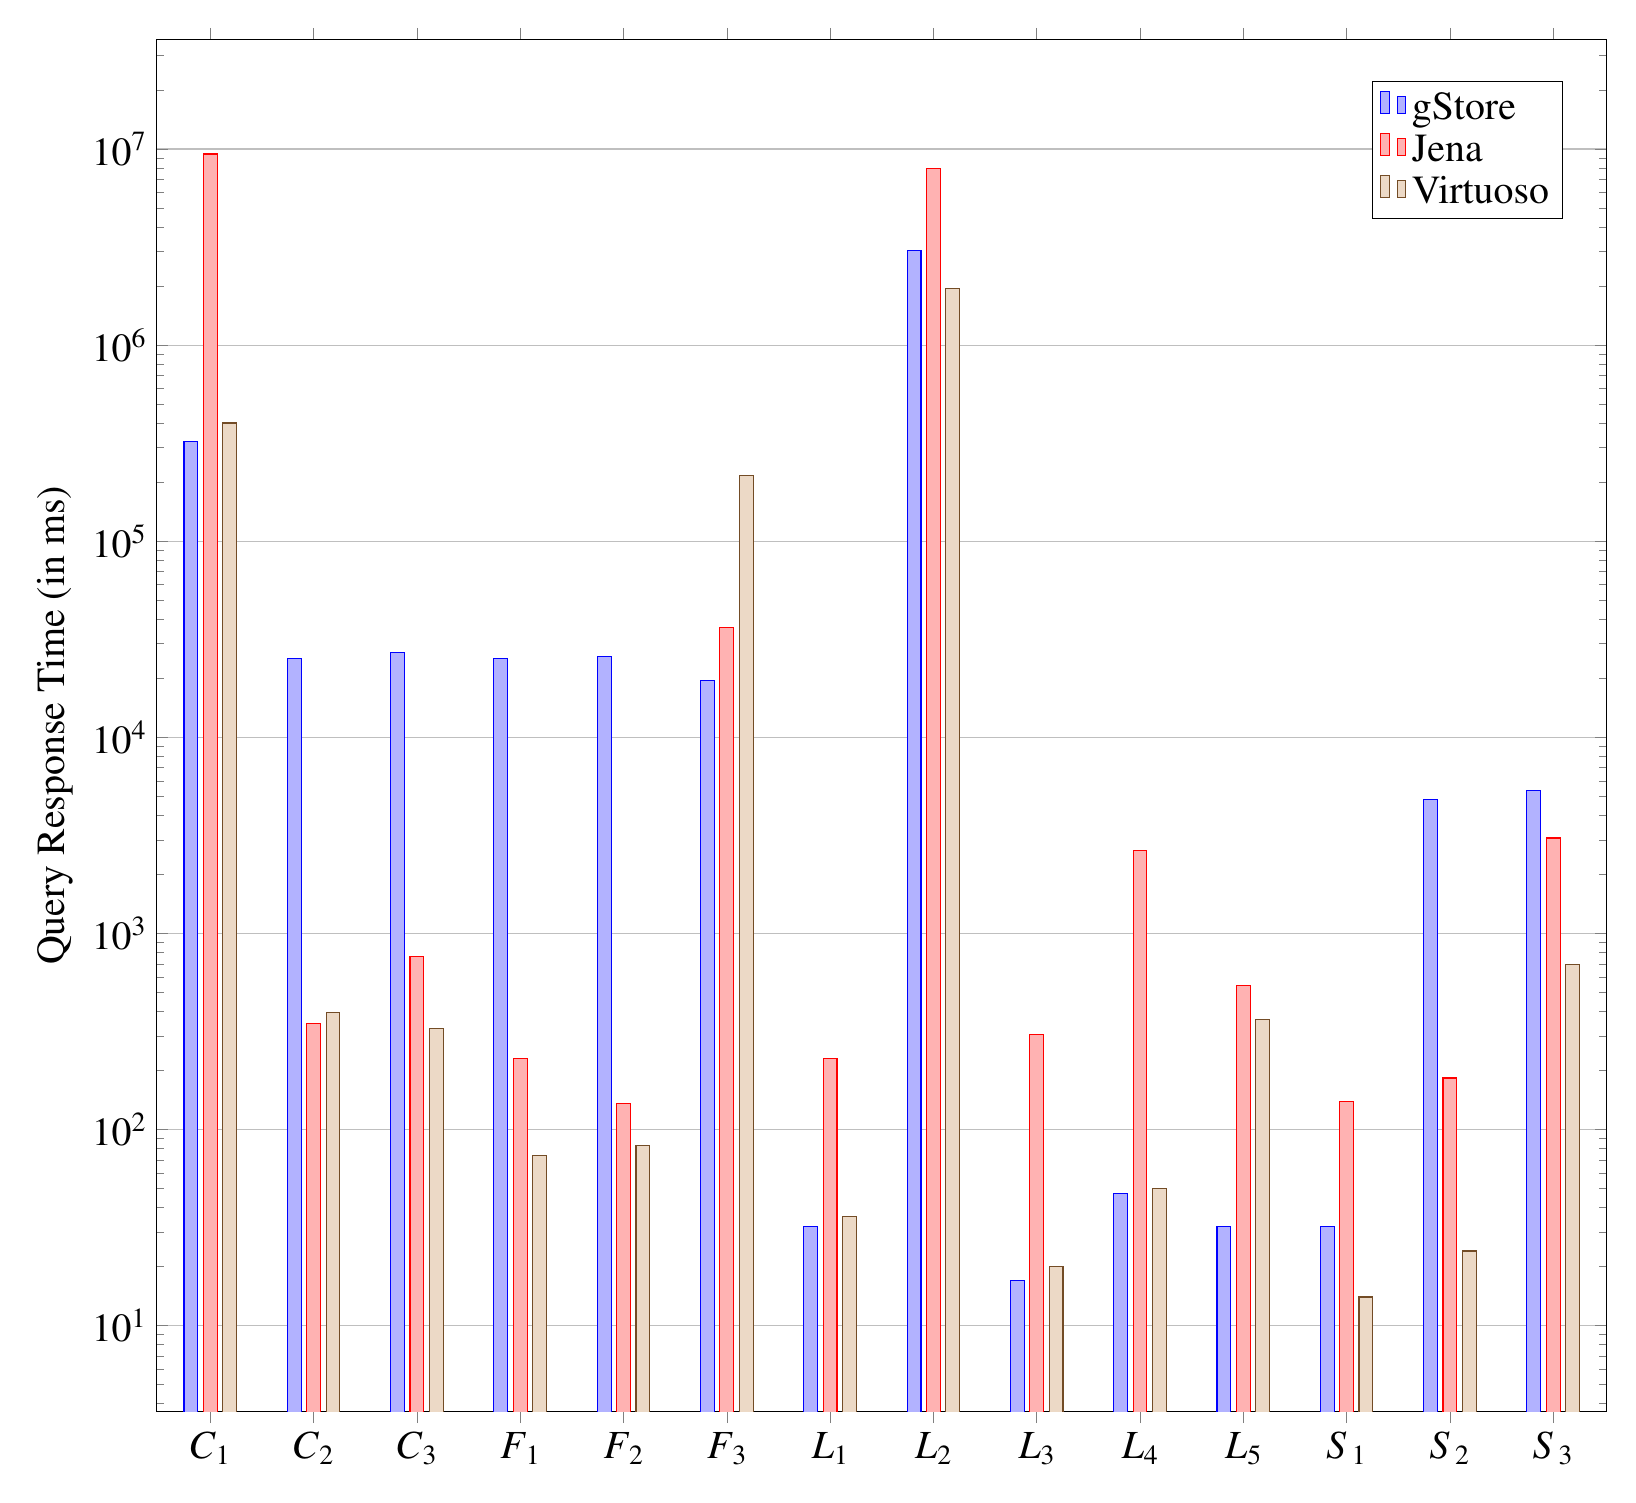
\begin{tikzpicture}[font=\Large]
 		 \begin{semilogyaxis}[
                width = 20cm,
               height = 19cm,
    			ybar,
   			ymajorgrids = true,
   			ylabel = {Query Response Time (in ms)},
                %xlabel = {Queries},
    			symbolic x coords = 
    			    	{$C_{1}$,$C_{2}$,$C_{3}$,$F_{1}$,$F_{2}$,$F_{3}$, $L_{1}$,$L_{2}$,$L_{3}$,$L_{4}$,$L_{5}$, $S_{1}$,$S_{2}$,$S_{3}$},
    bar width=5pt,
             enlarge x limits=0.04,
    			scaled y ticks = true,
			legend pos= north east,
 legend cell align=left
   		]
	  %\part{title}
	   \addplot coordinates {($C_{1}$, 324042) ($C_{2}$, 25094) ($C_{3}$, 26955) ($F_{1}$, 25147) ($F_{2}$, 25779) ($F_{3}$, 19410) ($L_{1}$, 32) ($L_{2}$, 3051565) ($L_{3}$, 17) ($L_{4}$, 47) ($L_{5}$, 32) ($S_{1}$, 32) ($S_{2}$, 4811) ($S_{3}$, 5361) };   
	   
	   \addplot coordinates {($C_{1}$, 9428609) ($C_{2}$, 348) ($C_{3}$, 764) ($F_{1}$, 231) ($F_{2}$, 135) ($F_{3}$, 36434) ($L_{1}$, 230) ($L_{2}$, 7961623) ($L_{3}$, 306) ($L_{4}$, 2637) ($L_{5}$, 544) ($S_{1}$, 139) ($S_{2}$, 183) ($S_{3}$, 3064) };   
	   
	   \addplot coordinates {($C_{1}$, 400589) ($C_{2}$, 394) ($C_{3}$, 329) ($F_{1}$, 74) ($F_{2}$, 83) ($F_{3}$, 217162) ($L_{1}$, 36) ($L_{2}$, 1940036) ($L_{3}$, 20) ($L_{4}$, 50) ($L_{5}$, 364) ($S_{1}$, 14) ($S_{2}$, 24) ($S_{3}$, 696) };		
	  		
   		 \legend{gStore,Jena,Virtuoso}
  		\end{semilogyaxis}
\end{tikzpicture}

		}
		\label{fig:freebase2BPerformance}%
	}%
	\caption{Query Performance over Freebase 2B}%
	\label{fig:freebasePerformance}
\end{figure}

\clearpage

\section{Modification}

We provide insertion and deletion in gStore v0.5.0.
You can either insert/delete from a given RDF file, or just run sparql queries to insert/delete something.
If you want to modify something, you need to delete it and reinsert.
The cost of insertion and deletion are recorded in table \ref{table:modify}, where the time unit is ms.
We first build the database from lubm500M dataset, and then remove the first 30000 triples of the dataset from teh database. Finally, we add the removed triples again to acquire a complete database.(The answers of queries are all right.)
%TODO:100-3000 triples per second?
%TODO:the time of insert and delete is not precise

\begin{table}[htbp]
	\centering
	\begin{tabular}{p{60pt}>{\raggedleft\arraybackslash}p{60pt}>{\raggedleft\arraybackslash}p{60pt}>{\raggedleft\arraybackslash}p{60pt}}
		\toprule
		Dataset & build & insert & delete \\
		\midrule
		lubm500M & 5,348,766 & 3,500,000 & 3,700,000 \\
		\bottomrule
	\end{tabular}
	\caption{Insertion and Deletion}
	\label{table:modify}
\end{table}

\begin{comment}
However, bugs do exist in insertion/deletion. 
When testing on lubm66M, the answer of q1.sql and q2.sql are not all right if the operation order is: build, delete, insert, query.
More precisely, a few results are lost, though the proportion is really small.
We do not care about the efficiency of insert/delete, but the correctness is a must, which means we will try to fix this bug
as quickly as possible.
\end{comment}

\clearpage

\section{Conclusion}

\emph{This section is not tested and updated in gStore v0.5.0.}

gStore can go well with RDF datasets which are in N-Triples format and TTL format, while the other database
management systems may come across some questions. In addition, gStore outperforms other systems
on many SPARQL queries. What is more, gStore is highly extensively because it uses graph model
instead of relational model. \\

However, there are also some shortcomings for gStore:
\begin{enumerate}
	\item RDF datasets in XML format are not supported
	\item the disk cost is high
	\item gStore is sometimes slower
\end{enumerate}

Besides, gStore v0.5.0 does not generate solutions for satellites which are not selected. 
This will speed up the query answering process, while not keeping so many duplicates in the result set.
For example, in below query, let's assume that ?s has only one unique answer, but ?o1 and ?o2 both have 10,000 answers.
In previous versions of gStore, there are 100,000,000 records in the result set because we have to find the answer of ?s and generate the solutions for ?o1 and ?o2, even if only ?s is selected in the sparql query.
However, in the v0.5.0, we find the answer of ?s and return directly. In this case, there won't be so many duplicates in the result set as before, but this is ok.
\begin{lstlisting}
select ?s where
{
	?s <linkTo> ?o1 .
	?s <produce> ?o2 .
}
\end{lstlisting}

Out of question, the performance of gStore can be improved a lot later. 
The future work is listed below:
\begin{enumerate}
	\item fix the problem in insertion/deletion 
	\item support datasets of 1 billion triples in a single machine(only 500 million now)
	\item add unit testing for the whole system(only black-box testing now)
	\item do code level optimization(for example, large loop in Join module)
	\item speed up the table join process using pipeline
\end{enumerate}

\clearpage

\section{Appendix}

%\begin{comment}
%\begin{lstlisting}[language={[ANSI]C},numbers=left,numberstyle=\tiny,keywordstyle=\color{blue!70},commentstyle=\color{red!50!green!50!blue!50},frame=shadowbox, rulesepcolor=\color{red!20!green!20!blue!20}] 
%	int main(int argc, char ** argv) 
%	{ 
%		
%		printf("Hello world! \n"); 
%		return 0; 
%	} 
%\end{lstlisting}


\subsection{WatDiv queries}\label{watdiv}

These queries come from \cite{DBLP:journals/vldb/PengZO0Z16}.

\subsubsection{C1.sql}

\begin{lstlisting}[language=SQL] 
SELECT ?v0 ?v4 ?v6 ?v7 WHERE 
{
	?v0 <http://schema.org/caption> ?v1 .
	?v0 <http://schema.org/text> ?v2 .
	?v0 <http://schema.org/contentRating> ?v3 .
	?v0 <http://purl.org/stuff/rev#hasReview> ?v4 .
	?v4 <http://purl.org/stuff/rev#title> ?v5 .
	?v4 <http://purl.org/stuff/rev#reviewer> ?v6 .
	?v7 <http://schema.org/actor> ?v6 .
	?v7 <http://schema.org/language> ?v8 .
}
\end{lstlisting} 

\subsubsection{C2.sql}

\begin{lstlisting}[language=SQL] 
SELECT ?v0 ?v3 ?v4 ?v8 WHERE 
{
	?v0 <http://schema.org/legalName> ?v1 .
	?v0 <http://purl.org/goodrelations/offers> ?v2 .
	?v2 <http://schema.org/eligibleRegion> <http://db.uwaterloo.ca/~galuc/wsdbm/Country5> .
	?v2 <http://purl.org/goodrelations/includes> ?v3 .
	?v4 <http://schema.org/jobTitle> ?v5 .
	?v4 <http://xmlns.com/foaf/homepage> ?v6 .
	?v4 <http://db.uwaterloo.ca/~galuc/wsdbm/makesPurchase> ?v7 .
	?v7 <http://db.uwaterloo.ca/~galuc/wsdbm/purchaseFor> ?v3 .
	?v3 <http://purl.org/stuff/rev#hasReview> ?v8 .
	?v8 <http://purl.org/stuff/rev#totalVotes> ?v9 .
}
\end{lstlisting}

\subsubsection{C3.sql}

\begin{lstlisting}[language=SQL] 
SELECT ?v0 WHERE 
{
	?v0 <http://db.uwaterloo.ca/~galuc/wsdbm/likes> ?v1 .
	?v0 <http://db.uwaterloo.ca/~galuc/wsdbm/friendOf> ?v2 .
	?v0 <http://purl.org/dc/terms/Location> ?v3 .
	?v0 <http://xmlns.com/foaf/age> ?v4 .
	?v0 <http://db.uwaterloo.ca/~galuc/wsdbm/gender> ?v5 .
	?v0 <http://xmlns.com/foaf/givenName> ?v6 .
}
\end{lstlisting}

\subsubsection{F1.sql}

\begin{lstlisting}[language=SQL] 
SELECT ?v0 ?v2 ?v3 ?v4 ?v5 WHERE 
{
	?v0 <http://ogp.me/ns#tag> <http://db.uwaterloo.ca/~galuc/wsdbm/Topic103> .
	?v0 <http://www.w3.org/1999/02/22-rdf-syntax-ns#type> ?v2 .
	?v3 <http://schema.org/trailer> ?v4 .
	?v3 <http://schema.org/keywords> ?v5 .
	?v3 <http://db.uwaterloo.ca/~galuc/wsdbm/hasGenre> ?v0 .
	?v3 <http://www.w3.org/1999/02/22-rdf-syntax-ns#type> <http://db.uwaterloo.ca/~galuc/wsdbm/ProductCategory2> .
}
\end{lstlisting}

\subsubsection{F2.sql}

\begin{lstlisting}[language=SQL] 
SELECT ?v0 ?v1 ?v2 ?v4 ?v5 ?v6 ?v7 WHERE 
{
	?v0 <http://xmlns.com/foaf/homepage> ?v1 .
	?v0 <http://ogp.me/ns#title> ?v2 .
	?v0 <http://www.w3.org/1999/02/22-rdf-syntax-ns#type> ?v3 .
	?v0 <http://schema.org/caption> ?v4 .
	?v0 <http://schema.org/description> ?v5 .
	?v1 <http://schema.org/url> ?v6 .
	?v1 <http://db.uwaterloo.ca/~galuc/wsdbm/hits> ?v7 .
	?v0 <http://db.uwaterloo.ca/~galuc/wsdbm/hasGenre> <http://db.uwaterloo.ca/~galuc/wsdbm/SubGenre35> .
}
\end{lstlisting}

\subsubsection{F3.sql}

\begin{lstlisting}[language=SQL] 
SELECT ?v0 ?v1 ?v2 ?v4 ?v5 ?v6 WHERE 
{
	?v0 <http://schema.org/contentRating> ?v1 .
	?v0 <http://schema.org/contentSize> ?v2 .
	?v0 <http://db.uwaterloo.ca/~galuc/wsdbm/hasGenre> <http://db.uwaterloo.ca/~galuc/wsdbm/SubGenre59> .
	?v4 <http://db.uwaterloo.ca/~galuc/wsdbm/makesPurchase> ?v5 .
	?v5 <http://db.uwaterloo.ca/~galuc/wsdbm/purchaseDate> ?v6 .
	?v5 <http://db.uwaterloo.ca/~galuc/wsdbm/purchaseFor> ?v0 .
}
\end{lstlisting}

\subsubsection{F4.sql}

\begin{lstlisting}[language=SQL]
select ?v0 ?v1 ?v2 ?v4 ?v5 ?v6 ?v7 ?v8 where {
?v0	<http://xmlns.com/foaf/homepage>	?v1 . 
?v2	<http://purl.org/goodrelations/includes>	?v0 . 
?v0	<http://ogp.me/ns#tag>	<http://db.uwaterloo.ca/~galuc/wsdbm/Topic60> . 
?v0	<http://schema.org/description>	?v4 . 
?v0	<http://schema.org/contentSize>	?v8 . 
?v7	<http://db.uwaterloo.ca/~galuc/wsdbm/likes>	?v0 . 
?v1	<http://schema.org/url>	?v5 . 
?v1	<http://db.uwaterloo.ca/~galuc/wsdbm/hits>	?v6 . 
?v1	<http://schema.org/language>	<http://db.uwaterloo.ca/~galuc/wsdbm/Language0> . 
} 
\end{lstlisting}

\subsubsection{F5.sql}

\begin{lstlisting}[language=SQL]
select ?v0 ?v1 ?v3 ?v4 ?v5 ?v6 where {
?v0	<http://purl.org/goodrelations/includes>	?v1 . 
<http://db.uwaterloo.ca/~galuc/wsdbm/Retailer661>	<http://purl.org/goodrelations/offers>	?v0 . 
?v0	<http://purl.org/goodrelations/price>	?v3 . 
?v0	<http://purl.org/goodrelations/validThrough>	?v4 . 
?v1	<http://ogp.me/ns#title>	?v5 . 
?v1	<http://www.w3.org/1999/02/22-rdf-syntax-ns#type>	?v6 . 
}
\end{lstlisting}

\subsubsection{L1.sql}

\begin{lstlisting}[language=SQL] 
SELECT ?v0 ?v2 ?v3 WHERE 
{
	?v0 <http://db.uwaterloo.ca/~galuc/wsdbm/subscribes> <http://db.uwaterloo.ca/~galuc/wsdbm/Website38303> .
	?v2 <http://schema.org/caption> ?v3 .
	?v0 <http://db.uwaterloo.ca/~galuc/wsdbm/likes> ?v2 .
}
\end{lstlisting}

\subsubsection{L2.sql}

\begin{lstlisting}[language=SQL] 
SELECT ?v1 ?v2 WHERE 
{
	<http://db.uwaterloo.ca/~galuc/wsdbm/City131> <http://www.geonames.org/ontology#parentCountry> ?v1 .
	?v2 <http://db.uwaterloo.ca/~galuc/wsdbm/likes> <http://db.uwaterloo.ca/~galuc/wsdbm/Product0> .
	?v2 <http://schema.org/nationality> ?v1 .
}
\end{lstlisting}

\subsubsection{L3.sql}

\begin{lstlisting}[language=SQL]
SELECT ?v0 ?v1 WHERE 
{
	?v0 <http://db.uwaterloo.ca/~galuc/wsdbm/likes> ?v1 .
	?v0 <http://db.uwaterloo.ca/~galuc/wsdbm/subscribes> <http://db.uwaterloo.ca/~galuc/wsdbm/Website20769> .
}
\end{lstlisting}

\subsubsection{L4.sql}

\begin{lstlisting}[language=SQL]
select ?v0 ?v2 where 
{
?v0	<http://ogp.me/ns#tag>	<http://db.uwaterloo.ca/~galuc/wsdbm/Topic117> . 
?v0	<http://schema.org/caption>	?v2 . 
}
\end{lstlisting}

\subsubsection{L5.sql}

\begin{lstlisting}[language=SQL]
select ?v0 ?v1 ?v3 where 
{
?v0	<http://schema.org/jobTitle>	?v1 . 
?v0	<http://schema.org/nationality>	?v3 . 
<http://db.uwaterloo.ca/~galuc/wsdbm/City22>	<http://www.geonames.org/ontology#parentCountry>	?v3 . 
}
\end{lstlisting}

\subsubsection{S1.sql}

\begin{lstlisting}[language=SQL]
SELECT ?v0 ?v1 ?v3 ?v4 ?v5 ?v6 ?v7 ?v8 ?v9 WHERE 
{
	?v0 <http://purl.org/goodrelations/includes> ?v1 .
	<http://db.uwaterloo.ca/~galuc/wsdbm/Retailer391> <http://purl.org/goodrelations/offers> ?v0 .
	?v0 <http://purl.org/goodrelations/price> ?v3 .
	?v0 <http://purl.org/goodrelations/serialNumber> ?v4 .
	?v0 <http://purl.org/goodrelations/validFrom> ?v5 .
	?v0 <http://purl.org/goodrelations/validThrough> ?v6 .
	?v0 <http://schema.org/eligibleQuantity> ?v7 .
	?v0 <http://schema.org/eligibleRegion> ?v8 .
	?v0 <http://schema.org/priceValidUntil> ?v9 .
}
\end{lstlisting}

\subsubsection{S2.sql}

\begin{lstlisting}[language=SQL]
SELECT ?v0 ?v1 ?v3 WHERE 
{
	?v0 <http://purl.org/dc/terms/Location> ?v1 .
	?v0 <http://schema.org/nationality> <http://db.uwaterloo.ca/~galuc/wsdbm/Country23> .
	?v0 <http://db.uwaterloo.ca/~galuc/wsdbm/gender> ?v3 .
	?v0 <http://www.w3.org/1999/02/22-rdf-syntax-ns#type> <http://db.uwaterloo.ca/~galuc/wsdbm/Role2> .
}
\end{lstlisting}

\subsubsection{S3.sql}

\begin{lstlisting}[language=SQL]
SELECT ?v0 ?v2 ?v3 ?v4 WHERE 
{
	?v0 <http://www.w3.org/1999/02/22-rdf-syntax-ns#type> <http://db.uwaterloo.ca/~galuc/wsdbm/ProductCategory12> .
	?v0 <http://schema.org/caption> ?v2 .
	?v0 <http://db.uwaterloo.ca/~galuc/wsdbm/hasGenre> ?v3 .
	?v0 <http://schema.org/publisher> ?v4 .
}
\end{lstlisting}

\subsubsection{S4.sql}

\begin{lstlisting}[language=SQL]
select ?v0 ?v2 ?v3 where 
{
?v0	<http://xmlns.com/foaf/age>	<http://db.uwaterloo.ca/~galuc/wsdbm/AgeGroup1> . 
?v0	<http://xmlns.com/foaf/familyName>	?v2 . 
?v3	<http://purl.org/ontology/mo/artist>	?v0 . 
?v0	<http://schema.org/nationality>	<http://db.uwaterloo.ca/~galuc/wsdbm/Country1> . 
}
\end{lstlisting}

\subsubsection{S5.sql}

\begin{lstlisting}[language=SQL]
select ?v0 ?v2 ?v3 where 
{
?v0	<http://www.w3.org/1999/02/22-rdf-syntax-ns#type>	<http://db.uwaterloo.ca/~galuc/wsdbm/ProductCategory3> . 
?v0	<http://schema.org/description>	?v2 . 
?v0	<http://schema.org/keywords>	?v3 . 
?v0	<http://schema.org/language>	<http://db.uwaterloo.ca/~galuc/wsdbm/Language0> . 
}
\end{lstlisting}

\subsubsection{S6.sql}

\begin{lstlisting}[language=SQL]
select ?v0 ?v1 ?v2 where 
{
?v0	<http://purl.org/ontology/mo/conductor>	?v1 . 
?v0	<http://www.w3.org/1999/02/22-rdf-syntax-ns#type>	?v2 . 
?v0	<http://db.uwaterloo.ca/~galuc/wsdbm/hasGenre>	<http://db.uwaterloo.ca/~galuc/wsdbm/SubGenre1> . 
}
\end{lstlisting}

\subsubsection{S7.sql}

\begin{lstlisting}[language=SQL]
select ?v0 ?v1 ?v2 where 
{
?v0	<http://www.w3.org/1999/02/22-rdf-syntax-ns#type>	?v1 . 
?v0	<http://schema.org/text>	?v2 . 
<http://db.uwaterloo.ca/~galuc/wsdbm/User2094>	<http://db.uwaterloo.ca/~galuc/wsdbm/likes>	?v0 .
}
\end{lstlisting}

\subsection{LUBM queries}\label{lubm}
%TODO;bib
This queries come from two places.
$q1 \sim q7$ come from \cite{Atre2010Matrix} and \cite{DBLP:journals/vldb/PengZO0Z16}.
$q8 \sim q21$ come from \cite{Guo2005LUBM} and \cite{Zou2014gStore}.

\subsubsection{q1.sql}

\begin{lstlisting}[language=SQL]
select ?x where
{
	?x      <rdf:type>      <ub:GraduateStudent>.
	?y      <rdf:type>      <ub:University>.
	?z      <rdf:type>      <ub:Department>.
	?x      <ub:memberOf>   ?z.
	?z      <ub:subOrganizationOf>  ?y.
	?x      <ub:undergraduateDegreeFrom>    ?y.
}
\end{lstlisting}

\subsubsection{q2.sql}

\begin{lstlisting}[language=SQL]
select ?x where
{
	?x      <rdf:type>      <ub:Course>.
	?x      <ub:name>       ?y.
}  
\end{lstlisting}

\subsubsection{q3.sql}

\begin{lstlisting}[language=SQL]
select ?x where
{
	?x      <rdf:type>      <ub:UndergraduateStudent>.
	?y      <rdf:type>      <ub:University>.
	?z      <rdf:type>      <ub:Department>.
	?x      <ub:memberOf>   ?z.
	?z      <ub:subOrganizationOf>  ?y.
	?x      <b:undergraduateDegreeFrom>     ?y.
}
\end{lstlisting}

\subsubsection{q4.sql}

\begin{lstlisting}[language=SQL]
elect ?x ?y1 ?y2 ?y3 where
{
	?x      <ub:worksFor>   <http://www.Department0.University0.edu>.
	?x      <rdf:type>      <ub:FullProfessor>.
	?x      <ub:name>       ?y1.
	?x      <ub:emailAddress>       ?y2.
	?x      <ub:telephone>  ?y3.
}
\end{lstlisting}

\subsubsection{q5.sql}

\begin{lstlisting}[language=SQL]
select ?x where
{
	?x      <ub:subOrganizationOf>  <http://www.Department0.University0.edu>.
	?x      <rdf:type>      <ub:ResearchGroup>.
}
\end{lstlisting}

\subsubsection{q6.sql}

\begin{lstlisting}[language=SQL]
select ?x ?y where
{
	?y      <ub:subOrganizationOf>  <http://www.University0.edu>.
	?y      <rdf:type>      <ub:Department>.
	?x      <ub:worksFor>   ?y.
	?x      <rdf:type>      <ub:FullProfessor>.
}
\end{lstlisting}

\subsubsection{q7.sql}

\begin{lstlisting}[language=SQL]
select ?x ?y ?z where
{
	?x      <rdf:type>      <ub:UndergraduateStudent>.
	?y      <rdf:type>      <ub:FullProfessor>.
	?z      <rdf:type>      <ub:Course>.
	?x      <ub:advisor>    ?y.
	?x      <ub:takesCourse>        ?z.
	?y      <ub:teacherOf>  ?z.
}
\end{lstlisting}

\subsubsection{q8.sql}

\begin{lstlisting}[language=SQL]
select ?X where
{
	?X      <rdf:type>      <ub:GraduateStudent>.
	?X      <ub:takesCourse>        <http://www.Department0.University0.edu/GraduateCourse0>.
}
\end{lstlisting}

\subsubsection{q9.sql}

\begin{lstlisting}[language=SQL]
select ?X ?Y ?Z where
{
	?X      <rdf:type>      <ub:GraduateStudent>.
	?Y      <rdf:type>      <ub:University>.
	?Z      <rdf:type>      <ub:Department>.
	?X      <ub:memberOf>   ?Z.
	?Z      <ub:subOrganizationOf>  ?Y.
	?X      <ub:undergraduateDegreeFrom>    ?Y.
}    
\end{lstlisting}

\subsubsection{q10.sql}

\begin{lstlisting}[language=SQL]
select ?X where
{
	?X      <rdf:type>      <ub:Publication>.
	?X      <ub:publicationAuthor>  <http://www.Department0.University0.edu/AssistantProfessor0>.
}
\end{lstlisting}

\subsubsection{q11.sql}

\begin{lstlisting}[language=SQL]
select ?Y1 ?Y2 ?Y3 where
{
	?X      <rdf:type>      <ub:FullProfessor>.
	?X      <ub:worksFor>   <http://www.Department0.University0.edu>.
	?X      <ub:name>       ?Y1.
	?X      <ub:emailAddress>       ?Y2.
	?X      <ub:telephone>  ?Y3.
}
\end{lstlisting}

\subsubsection{q12.sql}

\begin{lstlisting}[language=SQL]
select ?X where
{
	?X      <ub:memberOf>   <http://www.Department0.University0.edu>.
}
\end{lstlisting}

\subsubsection{q13.sql}

\begin{lstlisting}[language=SQL]
select ?X where
{
	?X      <rdf:type>      <ub:UndergraduateStudent>.
}
\end{lstlisting}

\subsubsection{q14.sql}

\begin{lstlisting}[language=SQL]
elect ?X ?Y where
{
	?X      <rdf:type>      <ub:Student>.
	?Y      <rdf:type>      <ub:Course>.
	?X      <ub:takesCourse>        ?Y.
	<http://www.Department0.University0.edu/AssociateProfessor0>    <ub:teacherOf>  ?Y.
}
\end{lstlisting}

\subsubsection{q15.sql}

\begin{lstlisting}[language=SQL]
select ?X where
{
	?X      <rdf:type>      <ub:UndergraduateStudent>.
	?Y      <rdf:type>      <ub:Department>.
	?X      <ub:memberOf>   ?Y.
	?Y      <ub:subOrganizationOf>  <http://www.University0.edu>.
	?X      <ub:emailAddress>       ?Z.
}
\end{lstlisting}

\subsubsection{q16.sql}

\begin{lstlisting}[language=SQL]
select ?X ?Y ?Z where
{
	?X      <rdf:type>      <ub:UndergraduateStudent>.
	?Z      <rdf:type>      <ub:Course>.
	?X      <ub:advisor>    ?Y.
	?Y      <ub:teacherOf>  ?Z.
	?X      <ub:takesCourse>        ?Z.
}
\end{lstlisting}

\subsubsection{q17.sql}

\begin{lstlisting}[language=SQL]
select ?X where
{
	?X      <rdf:type>      <ub:GraduateStudent>.
	?X      <ub:takesCourse>        <http://www.Department0.University0.edu/GraduateCourse0>.
}
\end{lstlisting}

\subsubsection{q18.sql}

\begin{lstlisting}[language=SQL]
select ?X where
{
	?X      <rdf:type>      <ub:ResearchGroup>.
	?X      <ub:subOrganizationOf>  <http://www.University0.edu>.
}
\end{lstlisting}

\subsubsection{q19.sql}

\begin{lstlisting}[language=SQL]
select ?X ?Y where
{
	?Y      <rdf:type>      <ub:Department>.
	?X      <ub:worksFor>   ?Y.
	?Y      <ub:subOrganizationOf>  <http://www.University0.edu>.
}
\end{lstlisting}

\subsubsection{q20.sql}

\begin{lstlisting}[language=SQL]
select ?X where
{
	<http://www.University0.edu>    <ub:undergraduateDegreeFrom>    ?X.
}
\end{lstlisting}

\subsubsection{q21.sql}

\begin{lstlisting}[language=SQL]
select ?X where
{
	?X      <rdf:type>      <ub:UndergraduateStudent>.
}
\end{lstlisting}



\subsection{DBpedia queries}\label{dbpedia}

%TODO:add bib, change these queries to formal ones
These queries are written by us, imitating queries in other benchmarks.

\subsubsection{q0.sql}

\begin{lstlisting}[language=SQL] 
select ?v0 where
{
	?v0 <http://www.w3.org/1999/02/22-rdf-syntax-ns#type> <http://dbpedia.org/class/yago/LanguagesOfBotswana> .
	?v0 <http://www.w3.org/1999/02/22-rdf-syntax-ns#type>    <http://dbpedia.org/class/yago/LanguagesOfNamibia> .
	?v0 <http://www.w3.org/1999/02/22-rdf-syntax-ns#type> <http://dbpedia.org/ontology/Language> .
}
\end{lstlisting}

\subsubsection{q1.sql}

\begin{lstlisting}[language=SQL] 
select ?v0 where
{
	?v0 <http://dbpedia.org/ontology/associatedBand> <http://dbpedia.org/resource/LCD_Soundsystem> .
}
\end{lstlisting}

\subsubsection{q2.sql}

\begin{lstlisting}[language=SQL] 
select ?v2 where
{
	<http://dbpedia.org/resource/!!Destroy-Oh-Boy!!> <http://dbpedia.org/property/title> ?v2 .
}
\end{lstlisting}

\subsubsection{q3.sql}

\begin{lstlisting}[language=SQL] 
select ?v0 ?v2 where
{
	?v0 <http://dbpedia.org/ontology/activeYearsStartYear> ?v2 .
}
\end{lstlisting}

\subsubsection{q4.sql}

\begin{lstlisting}[language=SQL] 
select ?v0 ?v1 ?v2 where
{
	?v0 <http://dbpedia.org/property/dateOfBirth> ?v2 .
	?v1 <http://dbpedia.org/property/genre> ?v2 .
}
\end{lstlisting}

\subsubsection{q5.sql}

\begin{lstlisting}[language=SQL] 
select ?v0 ?v1 ?v2 ?v3 where
{
	?v0 <http://dbpedia.org/property/familycolor> ?v1 .
	?v0 <http://dbpedia.org/property/glotto> ?v2 .
	?v0 <http://dbpedia.org/property/lc> ?v3 .
}
\end{lstlisting}

\subsubsection{q6.sql}

\begin{lstlisting}[language=SQL] 
select ?v0 ?v1 ?v2 ?v3 ?v4 ?v5 ?v6 ?v7 ?v8 ?v9 where
{
	?v0 <http://dbpedia.org/property/dateOfBirth> ?v1 .
	?v0 <http://dbpedia.org/property/genre> ?v2 .
	?v0 <http://dbpedia.org/property/instrument> ?v3 .
	?v0 <http://dbpedia.org/property/label> ?v4 .
	?v0 <http://dbpedia.org/property/placeOfBirth> ?v5 .
	?v6 <http://dbpedia.org/property/name> ?v7 .
	?v6 <http://dbpedia.org/property/occupation> ?v8 .
	?v6 <http://dbpedia.org/property/placeOfBirth> ?v5 .
	?v6 <http://dbpedia.org/property/instrument> ?v3 .
	?v6 <http://dbpedia.org/property/notableInstruments> ?v9 .
}
\end{lstlisting}

\clearpage

\subsection{BSBM queries}\label{bsbm}

These queries is written by us.

\subsubsection{q0.sql}

\begin{lstlisting}[language=SQL] 
select ?v0 where
{
?v0 <http://www4.wiwiss.fu-berlin.de/bizer/bsbm/v01/vocabulary/rating2> "6"^^<http://www.w3.org/2001/XMLSchema#integer> .
}
\end{lstlisting}

\subsubsection{q1.sql}

\begin{lstlisting}[language=SQL] 
select ?v0 ?v1 where
{
?v0 <http://www.w3.org/1999/02/22-rdf-syntax-ns#type> ?v1 .
}
\end{lstlisting}

\subsubsection{q2.sql}

\begin{lstlisting}[language=SQL] 
select ?v0 ?v1 where
{
?v0 <http://www.w3.org/2000/01/rdf-schema#label> ?v1 .
?v1 <http://purl.org/dc/elements/1.1/publisher> ?v2 .
}
\end{lstlisting}

\subsubsection{q3.sql}

\begin{lstlisting}[language=SQL] 
select ?v0 ?v1 ?v2 where
{
?v0 <http://purl.org/dc/elements/1.1/publisher> ?v1 .
?v0 <http://purl.org/dc/elements/1.1/date> ?v2 .
}
\end{lstlisting}

\subsubsection{q4.sql}

\begin{lstlisting}[language=SQL] 
select ?v0 ?v1 ?v2 where
{
?v0 <http://www.w3.org/2000/01/rdf-schema#label> ?v2 .
?v1 <http://www.w3.org/2000/01/rdf-schema#subClassOf> ?v2 .
}
\end{lstlisting}

\subsubsection{q5.sql}

\begin{lstlisting}[language=SQL] 
select ?v0 ?v1 ?v2 ?v3 where
{
?v0 <http://www.w3.org/2000/01/rdf-schema#label> ?v1 .
?v0 <http://www.w3.org/1999/02/22-rdf-syntax-ns#type> ?v2 .
?v3 <http://www.w3.org/2000/01/rdf-schema#label> ?v1 .
?v3 <http://purl.org/dc/elements/1.1/publisher> <http://www4.wiwiss.fu-berlin.de/bizer/bsbm/v01/instances/StandardizationInstitution1> .
}
\end{lstlisting}

\subsubsection{q6.sql}

\begin{lstlisting}[language=SQL] 
select ?v0 ?v1 ?v2 ?v3 ?v4 where
{
?v0 <http://www.w3.org/1999/02/22-rdf-syntax-ns#type> ?v1 .
?v0 <http://purl.org/dc/elements/1.1/date> ?v2 .
?v3 <http://www.w3.org/2000/01/rdf-schema#comment> ?v4 .
<http://www4.wiwiss.fu-berlin.de/bizer/bsbm/v01/instances/ProductType2> <http://www.w3.org/2000/01/rdf-schema#comment> ?v4 .
?v3 <http://www.w3.org/1999/02/22-rdf-syntax-ns#type> ?v1 .
}
\end{lstlisting}

\subsubsection{q7.sql}

\begin{lstlisting}[language=SQL] 
select ?v0 ?v1 ?v2 ?v3 ?v4 where
{
?v0 <http://purl.org/dc/elements/1.1/title> ?v1 .
?v0 <http://purl.org/dc/elements/1.1/publisher> <http://www4.wiwiss.fu-berlin.de/bizer/bsbm/v01/instances/dataFromRatingSite11/RatingSite11> .
?v0 <http://purl.org/stuff/rev#text> ?v4 .
?v2 <http://purl.org/stuff/rev#reviewer> ?v3 .
?v2 <http://purl.org/dc/elements/1.1/date> "2008-04-16"^^<http://www.w3.org/2001/XMLSchema#date> .
?v2 <http://purl.org/stuff/rev#text> ?v4
}
\end{lstlisting}

\subsubsection{q8.sql}

\begin{lstlisting}[language=SQL] 
select ?v0 ?v1 ?v2 ?v3 ?v4 ?v5 ?v6 where
{
?v0 <http://www.w3.org/2000/01/rdf-schema#subClassOf> ?v1 .
?v0 <http://purl.org/dc/elements/1.1/date> ?v2 .
?v3 <http://purl.org/dc/elements/1.1/publisher> ?v4 .
?v3 <http://www.w3.org/2000/01/rdf-schema#subClassOf> ?v1 .
?v5 <http://purl.org/dc/elements/1.1/publisher> ?v6 .
?v5 <http://purl.org/dc/elements/1.1/date> ?v2 .
}
\end{lstlisting}

\subsubsection{q9.sql}

\begin{lstlisting}[language=SQL] 
select ?v0 ?v1 ?v2 ?v3 ?v4 ?v5 ?v6 ?v7 ?v8 where
{
?v0 <http://purl.org/dc/elements/1.1/date> "2000-07-17"^^<http://www.w3.org/2001/XMLSchema#date> .
?v0 <http://purl.org/dc/elements/1.1/publisher> ?v1 .
?v0 <http://www.w3.org/2000/01/rdf-schema#label> ?v2 .
?v0 <http://www.w3.org/2000/01/rdf-schema#comment> ?v8 .
?v3 <http://www.w3.org/2000/01/rdf-schema#subClassOf> <http://www4.wiwiss.fu-berlin.de/bizer/bsbm/v01/instances/ProductType2> .
?v3 <http://purl.org/dc/elements/1.1/publisher> ?v1 .
?v3 <http://www.w3.org/2000/01/rdf-schema#label> ?v4 .
?v3 <http://www.w3.org/1999/02/22-rdf-syntax-ns#type> ?v7 .
?v5 <http://www.w3.org/2000/01/rdf-schema#label> ?v2 .
?v5 <http://purl.org/dc/elements/1.1/publisher> ?v6 .
?v5 <http://www.w3.org/1999/02/22-rdf-syntax-ns#type> ?v7 .
}
\end{lstlisting}

%\end{comment}
\clearpage

\subsection{Freebase queries}\label{freebase}

These queries is written by us.

\subsubsection{C1.sql}

\begin{lstlisting}[language=SQL] 
select ?s ?s2 where
{
?s  <http://www.w3.org/2000/01/rdf-schema#label>    ?o       .
?s <http://rdf.freebase.com/ns/type.object.type> ?s2 .
?s2  <http://www.w3.org/2000/01/rdf-schema#label>    ?o       .
}
\end{lstlisting} 

\subsubsection{C2.sql}

\begin{lstlisting}[language=SQL] 
select ?s ?o ?s2 where
{
?s  <http://www.w3.org/2000/01/rdf-schema#label>    ?o       .
?s  <http://rdf.freebase.com/ns/type.property.schema>       <http://rdf.freebase.com/ns/american_football.football_player>   .
?s  <http://rdf.freebase.com/ns/type.property.unique>       ?o2  .
?s <http://rdf.freebase.com/ns/type.object.type> ?s2 .
?s2  <http://rdf.freebase.com/ns/type.property.unique>       ?o2  .
?s2  <http://www.w3.org/2000/01/rdf-schema#range>    ?o3    .
}
\end{lstlisting}

\subsubsection{C3.sql}

\begin{lstlisting}[language=SQL] 
select ?s ?o ?s2 where
{
?s  <http://www.w3.org/2000/01/rdf-schema#label>    ?o       .
?s  <http://rdf.freebase.com/ns/type.property.schema>       <http://rdf.freebase.com/ns/american_football.football_player>   .
?s  <http://rdf.freebase.com/ns/type.property.unique>       ?o2  .
?s <http://rdf.freebase.com/ns/type.object.type> ?s2 .
?s2  <http://rdf.freebase.com/ns/type.property.unique>       ?o2  .
?s2  <http://www.w3.org/2000/01/rdf-schema#range>    <http://rdf.freebase.com/ns/type.enumeration>    .
?s2 <http://rdf.freebase.com/ns/type.property.expected_type> ?s3 .
?s3 <http://www.w3.org/2000/01/rdf-schema#domain> ?o3 .
}
\end{lstlisting}

\subsubsection{F1.sql}

\begin{lstlisting}[language=SQL] 
select ?s where
{
?s  <http://www.w3.org/2000/01/rdf-schema#label>    ?o       .
?s  <http://rdf.freebase.com/ns/type.property.schema>       <http://rdf.freebase.com/ns/american_football.football_player>   .
?s <http://rdf.freebase.com/ns/type.object.type> ?s2 .
?s2  <http://rdf.freebase.com/ns/type.property.unique>       "true"  .
?s2  <http://www.w3.org/2000/01/rdf-schema#range>    <http://rdf.freebase.com/ns/type.enumeration>    .
}
\end{lstlisting}

\subsubsection{F2.sql}

\begin{lstlisting}[language=SQL] 
select ?s where
{
?s  <http://www.w3.org/2000/01/rdf-schema#label>    ?o       .
?s  <http://rdf.freebase.com/ns/type.property.schema>       <http://rdf.freebase.com/ns/american_football.football_player>   .
?s <http://rdf.freebase.com/ns/type.object.type> ?s2 .
?s2  <http://rdf.freebase.com/ns/type.property.unique>       ?o2  .
?s2  <http://www.w3.org/2000/01/rdf-schema#range>    ?o3    .
}
\end{lstlisting}

\subsubsection{F3.sql}

\begin{lstlisting}[language=SQL] 
select ?o ?s2 where
{
?s  <http://www.w3.org/2000/01/rdf-schema#label>    ?o       .
?s  <http://rdf.freebase.com/ns/type.property.schema>       ?o4   .
?s <http://rdf.freebase.com/ns/type.object.type> ?s2 .
?s2  <http://rdf.freebase.com/ns/type.property.unique>       ?o2  .
?s2  <http://www.w3.org/2000/01/rdf-schema#range>    ?o3    .
}
\end{lstlisting}

\subsubsection{L1.sql}

\begin{lstlisting}[language=SQL] 
select ?s where
{
?s  <http://www.w3.org/2000/01/rdf-schema#label>    "footballdb ID"@en       .
}
\end{lstlisting}

\subsubsection{L2.sql}

\begin{lstlisting}[language=SQL] 
select ?s ?o where
{
?s <http://rdf.freebase.com/ns/type.object.name> ?o .
}
\end{lstlisting}

\subsubsection{L3.sql}

\begin{lstlisting}[language=SQL]
select ?s ?o where
{
?s <http://www.w3.org/2000/01/rdf-schema#domain> ?o .
?o <http://rdf.freebase.com/ns/type.object.name>   "footballdb ID"@en       .
}
\end{lstlisting}

\subsubsection{L4.sql}

\begin{lstlisting}[language=SQL]
select ?s ?s2 where
{
?s <http://www.w3.org/2000/01/rdf-schema#domain> ?o .
?o <http://rdf.freebase.com/ns/type.property.expected_type> ?s2 .
?s2  <http://rdf.freebase.com/ns/type.property.unique>       "true"  .
}
\end{lstlisting}

\subsubsection{L5.sql}

\begin{lstlisting}[language=SQL]
select ?s ?s2 where
{
?s <http://www.w3.org/2000/01/rdf-schema#domain> ?o .
?o <http://rdf.freebase.com/ns/type.property.expected_type> ?s2 .
?s2  <http://rdf.freebase.com/ns/type.property.unique>       ?o2  .
}
\end{lstlisting}

\subsubsection{S1.sql}

\begin{lstlisting}[language=SQL]
select ?s where
{
?s  <http://www.w3.org/2000/01/rdf-schema#label>    "footballdb ID"@en       .
?s  <http://rdf.freebase.com/ns/type.property.schema>       <http://rdf.freebase.com/ns/american_football.football_player>   .
?s  <http://rdf.freebase.com/ns/type.property.unique>       "true"  .
}
\end{lstlisting}

\subsubsection{S2.sql}

\begin{lstlisting}[language=SQL]
select ?o where
{
?s  <http://www.w3.org/2000/01/rdf-schema#label>    ?o       .
?s  <http://rdf.freebase.com/ns/type.property.schema>       <http://rdf.freebase.com/ns/american_football.football_player>   .
?s  <http://rdf.freebase.com/ns/type.property.unique>       ?o2  .
}
\end{lstlisting}

\subsubsection{S3.sql}

\begin{lstlisting}[language=SQL]
select ?s ?o where
{
?s  <http://www.w3.org/2000/01/rdf-schema#label>    ?o       .
?s  <http://rdf.freebase.com/ns/type.property.schema>       ?o2   .
?s  <http://rdf.freebase.com/ns/type.property.unique>       ?o3  .
}
\end{lstlisting}


\bibliographystyle{abbrv}
%\addtolength{\itemsep}{-1.5ex}
\bibliography{gstore}
\addcontentsline{toc}{section}{Reference}

\end{document}

